
\documentclass[twoside]{book}\usepackage[]{graphicx}\usepackage[]{xcolor}
%% maxwidth is the original width if it is less than linewidth
%% otherwise use linewidth (to make sure the graphics do not exceed the margin)
\makeatletter
\def\maxwidth{ %
  \ifdim\Gin@nat@width>\linewidth
    \linewidth
  \else
    \Gin@nat@width
  \fi
}
\makeatother

\definecolor{fgcolor}{rgb}{0.345, 0.345, 0.345}
\newcommand{\hlnum}[1]{\textcolor[rgb]{0.686,0.059,0.569}{#1}}%
\newcommand{\hlstr}[1]{\textcolor[rgb]{0.192,0.494,0.8}{#1}}%
\newcommand{\hlcom}[1]{\textcolor[rgb]{0.678,0.584,0.686}{\textit{#1}}}%
\newcommand{\hlopt}[1]{\textcolor[rgb]{0,0,0}{#1}}%
\newcommand{\hlstd}[1]{\textcolor[rgb]{0.345,0.345,0.345}{#1}}%
\newcommand{\hlkwa}[1]{\textcolor[rgb]{0.161,0.373,0.58}{\textbf{#1}}}%
\newcommand{\hlkwb}[1]{\textcolor[rgb]{0.69,0.353,0.396}{#1}}%
\newcommand{\hlkwc}[1]{\textcolor[rgb]{0.333,0.667,0.333}{#1}}%
\newcommand{\hlkwd}[1]{\textcolor[rgb]{0.737,0.353,0.396}{\textbf{#1}}}%

\usepackage{framed}
\makeatletter
\newenvironment{kframe}{%
 \def\at@end@of@kframe{}%
 \ifinner\ifhmode%
  \def\at@end@of@kframe{\end{minipage}}%
  \begin{minipage}{\columnwidth}%
 \fi\fi%
 \def\FrameCommand##1{\hskip\@totalleftmargin \hskip-\fboxsep
 \colorbox{shadecolor}{##1}\hskip-\fboxsep
     % There is no \\@totalrightmargin, so:
     \hskip-\linewidth \hskip-\@totalleftmargin \hskip\columnwidth}%
 \MakeFramed {\advance\hsize-\width
   \@totalleftmargin\z@ \linewidth\hsize
   \@setminipage}}%
 {\par\unskip\endMakeFramed%
 \at@end@of@kframe}
\makeatother

\definecolor{shadecolor}{rgb}{.97, .97, .97}
\definecolor{messagecolor}{rgb}{0, 0, 0}
\definecolor{warningcolor}{rgb}{1, 0, 1}
\definecolor{errorcolor}{rgb}{1, 0, 0}
\newenvironment{knitrout}{}{} % an empty environment to be redefined in TeX

\usepackage{alltt}
\usepackage[margin=.9in]{geometry}
%\usepackage{kpfonts}   % for \varhearsuit
%\usepackage{txfonts}    % for \varhearsuit
\usepackage{amsmath}
\usepackage{probstat}
\usepackage{booktabs}
\def\Tri{\distribution{Triangle}}
\def\Rayleigh{\distribution{Rayleigh}}
\def\SD{\operatorname{SD}}
\usepackage{xstring}
\usepackage{makeidx}

%\def\Prob{\operatorname{Pr}}
\def\tnot{\operatorname{not}}
\usepackage{hyperref}
\usepackage{graphicx}
\usepackage{tikz}
\usetikzlibrary{patterns}
\usepackage[hidenotes]{authNote}
\usepackage[answerdelayed,exercisedelayed,lastexercise,chapter]{problems}

%\def\myindex#1{\relax}
%\def\Rindex#1{\relax}
\def\myindex#1{\index{#1}}

\usepackage{multicol}
\usepackage{longtable}
\renewcommand{\arraystretch}{1.4}

\def\sfrac#1#2{#1/#2}
\newcommand{\Partial}[2]{\frac{\partial #1}{\partial #2}}


\usepackage[Bjornstrup]{fncychap}
\usepackage{fancyhdr}
\pagestyle{fancy}
\fancyhf{}

%% Now begin customising things. See the fancyhdr docs for more info.

\renewcommand{\chaptermark}[1]{\thispagestyle{fancy}\markboth{{#1}}{}}
\renewcommand{\sectionmark}[1]{\markright{{#1}}{}}
%\renewcommand{\headrulewidth}{0pt}

\newcommand{\exampleidx}[1]{{\it #1}}
\newcommand{\defidx}[1]{{\bf #1}}
\newcommand{\mainidx}[1]{{\bf #1}}
\newcommand{\probidx}[1]{{{\underline{#1}}}}

\newcommand{\variable}[1]{{\color{green!50!black}\texttt{#1}}}
%\newcommand{\dataframe}[1]{{\color{blue!80!black}\texttt{#1}}}
%\newcommand{\Rindex}[2][black]{\index{{\color{#1}\texttt{#2}}}}
\newcommand{\Rindex}[1]{\index{\texttt{#1}}}
\newcommand{\dataframe}[1]{{\color{blue!80!black}\texttt{#1}}\Rindex{#1}}
\newcommand{\function}[1]{{\color{purple!75!blue}\texttt{\StrSubstitute{#1}{()}{}()}}\Rindex{#1}}
\newcommand{\option}[1]{{\color{brown!80!black}\texttt{#1}}}
\newcommand{\argument}[1]{{\color{brown!80!black}\texttt{#1}}}
%\newcommand{\pkg}[1]{{\color{red!80!black}\texttt{#1}}}
\newcommand{\pkg}[1]{{\color{red!80!black}\texttt{#1}}\Rindex{#1}}
\renewcommand{\code}[1]{{\color{blue!80!black}\texttt{#1}}}
% and for models
\newcommand{\model}[2]{{$\,$\hbox{#1}\ \ensuremath{\sim}\ \hbox{#2}}}

\DeclareSymbolFont{extraup}{U}{zavm}{m}{n}
\DeclareMathSymbol{\varheartsuit}{\mathalpha}{extraup}{86}
\DeclareMathSymbol{\vardiamondsuit}{\mathalpha}{extraup}{87}

\chead{}
\lhead[\sf \thepage]{\sf \leftmark}
\rhead[\sf \leftmark]{\sf \thepage}
\lhead[\sf \thepage]{\sf \thechapter. \leftmark}
\rhead[\sf \thechapter. \leftmark]{\sf \thepage}
\cfoot{}
\lfoot[\sf Last Modified: \today]{\sf STAT243 : Spring 2016 : DeRuiter}
\rfoot[\sf STAT243 : Spring 2016 : DeRuiter]{\sf Last Modified: \today}

\pagestyle{fancy}

\usepackage{sfsect}
\usepackage{relsize}

%%%%%%%%%%%%%%%%%%%%%%%%%%%%%%% macros %%%%%%%%%%%%%%%%%%%%%%%%%%%%%%%%%%%%%%%%%%

\def\Chapter#1{%
\chapter{#1}
%\setcounter{page}{1}%
}
\def\R{{\sf R}}
\def\Rstudio{{\sf RStudio}}
\def\term#1{\textbf{#1}}
\def\tab#1{{\sf #1}}


\newlength{\tempfmlength}
\newsavebox{\fmbox}
\newenvironment{fmpage}[1]
     {
	 \medskip
	 \setlength{\tempfmlength}{#1}
	 \begin{lrbox}{\fmbox}
	   \begin{minipage}{#1}
		 \vspace*{.02\tempfmlength}
		 \hfill
	   \begin{minipage}{.95 \tempfmlength}}
		 {\end{minipage}\hfill
		 \vspace*{.015\tempfmlength}
		 \end{minipage}\end{lrbox}\fbox{\usebox{\fmbox}}
	 \medskip
	 }


\newenvironment{boxedText}[1][.98\textwidth]%
{%
\begin{center}
\begin{fmpage}{#1}
}%
{%
\end{fmpage}
\end{center}
}

\newenvironment{boxedTable}[2][tbp]%
{%
\begin{table}[#1]
  \refstepcounter{table}
  \begin{center}
\begin{fmpage}{.98\textwidth}
  \begin{center}
	\sf \large Box~\expandafter\thetable. #2
\end{center}
\medskip
}%
{%
\end{fmpage}
\end{center}
\end{table}		% need to do something about exercises that follow boxedTable
}

\def\question{{\sf Q. }}
\def\answer{{\sf A. }}

\newcounter{example}[section]

\newenvironment{example}%
{\refstepcounter{example}%
\textbf{Example \thesection.\arabic{example}. }}%
{}

\newenvironment{examples}%
{\refstepcounter{example}%
\textbf{Examples \thesection.\arabic{example}. }}%
{}

\renewcommand{\theexample}{\thesection.\arabic{example}}



\newif\ifsolutions
\solutionstrue
\solutionsfalse

\newif\ifsolutionslocal
\solutionslocaltrue
\solutionslocalfalse

\parindent=0pt
\parskip=3mm





%%%%%%%%%%%%%%%%%%%%%% title page info %%%%%%%%%%%%%%%%%%%%%%%%%%%%%%

\title{STAT243: Intro Stats}

\author{S DeRuiter (slightly modified from an original by R Pruim)}

\date{Spring 2016}

%%%%%%%%%%%%%%%%%%%%%%%%%%%%%%%%%%%%%%%%%%%%%%%%%%%%%%%%%%%%%%%%%%%%%
\makeindex
%%%%%%%%%%%%%%%%%%%%%%%%%%%%%%%%%%%%%%%%%%%%%%%%%%%%%%%%%%%%%%%%%%%%%

\lhead[\sf \thepage]{\sf \thechapter. \leftmark}
\rhead[\sf \thechapter. \leftmark]{\sf \thepage}
\IfFileExists{upquote.sty}{\usepackage{upquote}}{}
\begin{document}


\maketitle

\let\savecleardoublepage\cleardoublepage
\let\cleardoublepage\clearpage 

\setcounter{tocdepth}{1}
\tableofcontents

\let\cleardoublepage\savecleardoublepage

%%%%%%%%%%%%%%%%%%%%%%%%%%%%% 
%  main content starts here 
%%%%%%%%%%%%%%%%%%%%%%%%%%%%%%%




\Chapter{Random Variables and Probability}

\section{Key Definitions and Ideas}

\begin{description}
\item[random process]
A repeatable process that has multiple unpredictable potential outcomes.

Although we sometimes use language that suggests that a \emph{particular result} is 
random, it is really the \emph{process} that is random, not its results.

\item[outcome]
A potential result of a random process.

\item[sample space]
The set of all possible potential outcomes of a random process.

\item[event]
A subset of the sample space.  
That is, a set of outcomes (possibly all or none of the outcomes).

Statisticians often use capital letters from the beginning of the alphabet
for events.

\item[trial] One repetition of a random process.

\item[mutually exclusive] events.
Events that cannot happen on the same trial.

\item[probability] A numerical value between 0 and 1 assigned to 
an event to indicate how often the event occurs (in the long run).

\item[random variable]
A random variable is a variable whose value is a numerical outcome of a random process.

Examples of random variables: 
\begin{itemize}
\item
Roll a die and record the number.
\item
Roll two dice and record the sum.
\item
Flip 100 coins and count the number of heads.
\item
Sample 1000 people and count how many approve of the job the president is doing.
\item Sample 100 people and measure how long their right toenail is in mm. (Is this a good example or not?  It's a topic for discussion...)
\end{itemize}

Note: Statisticians usually use capital letters (often from the end of the alphabet)
for random variables, like this:  
Let $X$ be the number of heads in 10 flips of a fair coin.  What is $\Prob(X=5)$?


\item[probability distribution]
The distribution of a random variable.
(Remember that a distribution describes \emph{what values?} and 
\emph{with what freqency?})
\end{description}

As an example of a probability distribution, we can first consider a \emph{discrete} random variable.  Most of the examples of random variables given above are discrete. In other words, the values they can take on come from a set containing a finite number of possible values.  For example, if you roll a 6-sided die and record the number that comes up, there are only size possible outcomes, which are equally likely: the integers 1, 2, 3, 4, 5 and 6.  For discrete random variables, the probability distribution shows all the possible values on the x-axis, and the likelihood of observing each of those values on the y-axis.  Since there are a finite number of possible values that can be observed, these likelihoods are actually the \emph{probabilities} of observing each outcome, and the sum of all the probabilities must be 1.  For our example, where we rolled a die and recorded the value:

\begin{knitrout}
\definecolor{shadecolor}{rgb}{0.969, 0.969, 0.969}\color{fgcolor}

{\centering \includegraphics[width=\maxwidth]{figures/fig-discrete_pmf-1} 

}



\end{knitrout}

Things are a bit more complicated for \emph{continuous} random variables (the ones that can take on any numerical value).  Here, there sample space (the set of possible distinct values the random variable can take on) is infinite.  One consequence of this fact is that the interpretation of the y-axis values of the probability distribution changes.  The y-axis will still indicate the relative likelihood of observing any given value of the random variable.  However, here the random variable can take on an infinite number of possible values.  In this case, we can't interpret the y-axis values as probabilities.  They y axis units are called ``Likelihood" or "Density", and they indicate the relative frequency of each outcome. 

For a densityplot, which shows a smoothed version of the silhouette of a histogram (take STAT 343 and/or read about Kernel Density Estimation if you want a better explanation), Density is scaled such that the integral over all possible x-values (the area under the curve) is 1. For a histogram, Density is relative frequency, scaled so that the total area of all the boxes added together is 1.  We can think of the histograms and density plots we have been creating using continuous variables from R datasets as attempts to use data to approximate the distributions of random variables.  

For example, we might consider the growth of flower petals of the iris \textit{Iris setosa} as a random process, and let \texttt{X} be a random variable that is the length of each iris petal.  We could plot a histogram to approximate the distribution of \texttt{X} using the variable \texttt{Petal.Length} from the \dataframe{iris} data (from the \pkg{datasets} package in base R).

\begin{knitrout}
\definecolor{shadecolor}{rgb}{0.969, 0.969, 0.969}\color{fgcolor}

{\centering \includegraphics[width=\maxwidth]{figures/fig-cont_pdf-1} 

}



\end{knitrout}

\newpage

\section{Calculating Probabilities Empirically}

We would like to calculate the probability of an event
$A$, denoted $\Prob(A)$.

In the next section, we will see how to calculate probabilities based on the Axioms of probability, and logic.  But first, we will consider ways to make the calculations empirically -- based on observing many repetitions of a random process (in real life or in a computer simulation) and observing how often an event of interest occurs.

Random processes are repeatable, so practically, we can calculate empirical probabilities by simply repeating the process
over and over and keeping track of how often the event $A$ occurs.
For example, we could flip a coin 10,000 times and see what fraction 
are heads.\footnote{This has actually been done a couple of times 
in history, including once by mathematician John Kerrich while he was a prisoner of war during World War II.}

\[
\mbox{Empirical Probability} = 
\frac{\mbox{number of times $A$ occured}}
{\mbox{number of times random process was repeated}}
\]

Modern computing provides another way to compute empirical probabilities.
If we can simulate our random process on a computer, then we can 
repeat the process many times very quickly.  

\begin{example}
\question
What is the probability of getting exactly 5 heads 
if you flip a fair coin 10 times?  Using our random variable notation, let $X$ 
be the number of heads in 10 flips of a fair coin.  We want to know $\Prob(X=5)$.

\answer 
The \function{rflip()} function simulates flipping a coin as many times as we like.
\begin{knitrout}
\definecolor{shadecolor}{rgb}{0.969, 0.969, 0.969}\color{fgcolor}\begin{kframe}
\begin{alltt}
\hlkwd{rflip}\hlstd{(}\hlnum{10}\hlstd{)}
\end{alltt}
\begin{verbatim}
## 
## Flipping 10 coins [ Prob(Heads) = 0.5 ] ...
## 
## T H T H T H T T H T
## 
## Number of Heads: 4 [Proportion Heads: 0.4]
\end{verbatim}
\end{kframe}
\end{knitrout}
The \function{do()} function allows us to execute an R command ("do" somthing in R) over and over, as many times as we choose.  Here, our \function{rflip()} command simulates 10 coin-flips.  First we'll "do" our command three times and show the results.  

Then we'll do it 10,000 times and store the results in a variable called \texttt{tosses}, so we 
can create a table and a plot showing the empirical distribution.
\begin{knitrout}
\definecolor{shadecolor}{rgb}{0.969, 0.969, 0.969}\color{fgcolor}\begin{kframe}
\begin{alltt}
\hlkwd{do}\hlstd{(}\hlnum{3}\hlstd{)} \hlopt{*} \hlkwd{rflip}\hlstd{(}\hlnum{10}\hlstd{)}
\end{alltt}
\begin{verbatim}
##    n heads tails prop
## 1 10     3     7  0.3
## 2 10     7     3  0.7
## 3 10     5     5  0.5
\end{verbatim}
\begin{alltt}
\hlstd{tosses} \hlkwb{<-} \hlkwd{do}\hlstd{(}\hlnum{10000}\hlstd{)} \hlopt{*} \hlkwd{rflip}\hlstd{(}\hlnum{10}\hlstd{)}
\hlkwd{tally}\hlstd{(}\hlopt{~}\hlstd{heads,} \hlkwc{data} \hlstd{= tosses,} \hlkwc{format} \hlstd{=} \hlstr{"prop"}\hlstd{)}
\end{alltt}
\begin{verbatim}
## 
##      0      1      2      3      4      5      6      7      8      9     10 
## 0.0014 0.0084 0.0435 0.1239 0.2035 0.2462 0.1977 0.1213 0.0420 0.0112 0.0009
\end{verbatim}
\begin{alltt}
\hlkwd{histogram}\hlstd{(}\hlopt{~}\hlstd{heads,} \hlkwc{data} \hlstd{= tosses,} \hlkwc{width} \hlstd{=} \hlnum{1}\hlstd{)}
\end{alltt}
\end{kframe}

{\centering \includegraphics[width=\maxwidth]{figures/fig-coin-tosses-1} 

}



\end{knitrout}


Based on this sample, we would estimate that 
$\Prob(X=5) \approx 0.2462$.
\end{example}

\begin{example}
\question Use simulations to estimate the probability of rolling doubles
using two fair standard dice.

\answer
We can simulate rolling a die with the following code:
\begin{knitrout}
\definecolor{shadecolor}{rgb}{0.969, 0.969, 0.969}\color{fgcolor}\begin{kframe}
\begin{alltt}
\hlnum{1}\hlopt{:}\hlnum{6}  \hlcom{# the numbers 1 through 6}
\end{alltt}
\begin{verbatim}
## [1] 1 2 3 4 5 6
\end{verbatim}
\begin{alltt}
\hlkwd{resample}\hlstd{(}\hlnum{1}\hlopt{:}\hlnum{6}\hlstd{,} \hlnum{10}\hlstd{)}  \hlcom{# ten rolls of a 6-sided die}
\end{alltt}
\begin{verbatim}
##  [1] 4 5 6 5 2 1 2 6 1 4
\end{verbatim}
\end{kframe}
\end{knitrout}
The first 2 input arguments of \function{resample()} are \texttt{x} (the set of values from which you want to resample) and \texttt{size} (the number of items to choose from \texttt{x}).  You can also think of \texttt{size} as the number of \emph{times} to sample from \texttt{x}, if you are imagining sampling one item from \texttt{x} each time.

If we do this 10,000 times for each of two dice...
\begin{knitrout}
\definecolor{shadecolor}{rgb}{0.969, 0.969, 0.969}\color{fgcolor}\begin{kframe}
\begin{alltt}
\hlstd{die1} \hlkwb{<-} \hlkwd{resample}\hlstd{(}\hlnum{1}\hlopt{:}\hlnum{6}\hlstd{,} \hlnum{10000}\hlstd{)}
\hlstd{die2} \hlkwb{<-} \hlkwd{resample}\hlstd{(}\hlnum{1}\hlopt{:}\hlnum{6}\hlstd{,} \hlnum{10000}\hlstd{)}
\hlcom{# let's check that things look reasonable}
\hlkwd{head}\hlstd{(die1)}
\end{alltt}
\begin{verbatim}
## [1] 2 1 5 4 4 1
\end{verbatim}
\begin{alltt}
\hlkwd{head}\hlstd{(die2)}
\end{alltt}
\begin{verbatim}
## [1] 4 2 2 6 2 1
\end{verbatim}
\end{kframe}
\end{knitrout}
Then we can tabulate how often the two numbers matched in one of two ways:
\begin{knitrout}
\definecolor{shadecolor}{rgb}{0.969, 0.969, 0.969}\color{fgcolor}\begin{kframe}
\begin{alltt}
\hlkwd{tally}\hlstd{(}\hlopt{~}\hlstd{(die1} \hlopt{==} \hlstd{die2))}  \hlcom{# NOTE the double == here}
\end{alltt}
\begin{verbatim}
## 
##  TRUE FALSE 
##  1652  8348
\end{verbatim}
\begin{alltt}
\hlkwd{prop}\hlstd{(}\hlopt{~}\hlstd{(die1} \hlopt{==} \hlstd{die2))}  \hlcom{# NOTE the double == here}
\end{alltt}
\begin{verbatim}
##   TRUE 
## 0.1652
\end{verbatim}
\end{kframe}
\end{knitrout}
So the probability appears to be approximately 0.1652.

\end{example}


\begin{example}
\question
	Use simulation to estimate the probability of rolling a sum of 8 when rolling two fair six-sided dice.

\answer
We have already generated 10000 random rolls, so let's just reuse them.  (Alternatively, we could generate new rolls.)
\begin{knitrout}
\definecolor{shadecolor}{rgb}{0.969, 0.969, 0.969}\color{fgcolor}\begin{kframe}
\begin{alltt}
\hlstd{s} \hlkwb{<-} \hlstd{die1} \hlopt{+} \hlstd{die2}
\hlcom{# R adds element-wise: first entry of die1 + first of die2, second to second, etc.}
\hlkwd{prop}\hlstd{(}\hlopt{~}\hlstd{(s} \hlopt{==} \hlnum{8}\hlstd{))}
\end{alltt}
\begin{verbatim}
##   TRUE 
## 0.1357
\end{verbatim}
\end{kframe}
\end{knitrout}

We can estimate the probability of any sum the same way.
\begin{knitrout}
\definecolor{shadecolor}{rgb}{0.969, 0.969, 0.969}\color{fgcolor}\begin{kframe}
\begin{alltt}
\hlkwd{tally}\hlstd{(}\hlopt{~}\hlstd{s)}
\end{alltt}
\begin{verbatim}
## 
##    2    3    4    5    6    7    8    9   10   11   12 
##  296  555  816 1057 1416 1692 1357 1135  814  588  274
\end{verbatim}
\begin{alltt}
\hlcom{# if we are too lazy to divide by 10000 ourselves:}
\hlkwd{tally}\hlstd{(}\hlopt{~}\hlstd{s,} \hlkwc{format} \hlstd{=} \hlstr{"percent"}\hlstd{)}
\end{alltt}
\begin{verbatim}
## 
##     2     3     4     5     6     7     8     9    10    11    12 
##  2.96  5.55  8.16 10.57 14.16 16.92 13.57 11.35  8.14  5.88  2.74
\end{verbatim}
\end{kframe}
\end{knitrout}

Here's a slightly fancier version that puts all the information into a data frame.  Note the use of the function \function{data.frame()} to create the data table:
\begin{knitrout}
\definecolor{shadecolor}{rgb}{0.969, 0.969, 0.969}\color{fgcolor}\begin{kframe}
\begin{alltt}
\hlstd{rolls} \hlkwb{<-} \hlkwd{data.frame}\hlstd{(}\hlkwc{first} \hlstd{= die1,} \hlkwc{second} \hlstd{= die2,} \hlkwc{sum} \hlstd{= die1} \hlopt{+} \hlstd{die2)}
\hlkwd{head}\hlstd{(rolls)}
\end{alltt}
\begin{verbatim}
##   first second sum
## 1     2      4   6
## 2     1      2   3
## 3     5      2   7
## 4     4      6  10
## 5     4      2   6
## 6     1      1   2
\end{verbatim}
\begin{alltt}
\hlkwd{tally}\hlstd{(}\hlopt{~}\hlstd{sum,} \hlkwc{data} \hlstd{= rolls,} \hlkwc{format} \hlstd{=} \hlstr{"proportion"}\hlstd{)}
\end{alltt}
\begin{verbatim}
## 
##      2      3      4      5      6      7      8      9     10     11     12 
## 0.0296 0.0555 0.0816 0.1057 0.1416 0.1692 0.1357 0.1135 0.0814 0.0588 0.0274
\end{verbatim}
\begin{alltt}
\hlkwd{histogram}\hlstd{(}\hlopt{~}\hlstd{sum,} \hlkwc{data} \hlstd{= rolls,} \hlkwc{width} \hlstd{=} \hlnum{1}\hlstd{)}  \hlcom{# setting width is important for integer data}
\end{alltt}
\end{kframe}

{\centering \includegraphics[width=\maxwidth]{figures/fig-unnamed-chunk-7-1} 

}



\end{knitrout}
\end{example}

\section{Calculating Probabilities Theoretically}

The theoretical method combines
\begin{enumerate}
\item Some basic facts about probability (the Probability Axioms and Rules),
\item Some assumptions about the particular situation at hand, and 
\item Mathematical reasoning (arithmetic, algebra, logic, etc.).
\end{enumerate}

\subsection{The Three Probability Axioms}

Let $S$ be the sample space and let $A$ and $B$ be events.
\begin{enumerate}
\item Probability is between 0 and 1: $0 \le \Prob(A) \le 1$.
\item The probability of the sample space is 1: $\Prob(S) = 1$.
\item Additivity: 
If $A$ and $B$ are mutually exclusive, then 
$\Prob(A \tor B) = \Prob(A) + \Prob(B)$.
\end{enumerate}

\subsubsection{Notation Notes}
$\Prob(A \tor B)$ is the probability that either $A$ or $B$ (or both) 
occurs.  Often this is written $\Prob(A \union B)$.  $A \union B$ is usually read
``$A$ union $B$''.  The union of two sets is the set that contains all elements of both sets.

$\Prob(A \tand B)$ is the probability that \emph{both} $A$ and $B$ occur.
This is also written $\Prob (A \intersect B)$.  $A \intersect B$ is usually read
``$A$ intersect $B$''.  

Saying that $A$ and $B$ are mutually exclusive is the same as saying that there are no
outcomes in $A\intersect B$, i.e., that $A \intersect B = \emptyset$.

\subsection{Other Probability Rules}
These rules all follow from the axioms (although we will not necessarily prove them all here).
\subsubsection*{The Addition Rule}

If events $A$  and $B$ are mutually exclusive, then 
\[
\Prob(A \tor B) = \Prob(A) + \Prob(B)
\; .
\]

More generally,
\[
\Prob(A \tor B) = \Prob(A) + \Prob(B) - \Prob(A \tand B)
\; .
\]


\subsubsection*{The Complement Rule}

\[
\Prob(\tnot A) = 1 - \Prob(A)
\]


\subsubsection*{The Equally Likely Rule}

If the sample space consists of $n$ equally likely outcomes, then
the probability of an event $A$ is given by
\[
\Prob(A) = \frac{ \mbox{number of outcomes in $A$}}{n}
=\frac{ \card{A} }{\card{S} }\; .
\]

\emph{Warning:} One of the most common mistakes in probability is to apply this rule
when the outcomes are not equally likely.

\begin{examples}
\begin{enumerate}
\item Coin Toss: $\Prob(\mbox{heads}) = \frac{1}{2}$ if heads and tails are 
equally likely.
\item Rolling a Die: $\Prob(\mbox{even}) = \frac{3}{6}$ if the die is 
fair (each of the six numbers equally likely to occur).
\item
Sum of two Dice: the sum is a number between 2 and 12, but these numbers
are NOT equally likely.  

There are 36 equally likely combinations of two dice:

\begin{center}
\large
\begin{tabular}{|*{6}{c|}}
\hline
1,1 & 2,1 & 3,1 & 4,1 & 5,1 & 6,1 
\\ \hline
1,2 & 2,2 & 3,2 & 4,2 & 5,2 & 6,2 
\\ \hline
1,3 & 2,3 & 3,3 & 4,3 & 5,3 & 6,3 
\\ \hline
1,4 & 2,4 & 3,4 & 4,4 & 5,4 & 6,4 
\\ \hline
1,5 & 2,5 & 3,5 & 4,5 & 5,5 & 6,5 
\\ \hline
1,6 & 2,6 & 3,6 & 4,6 & 5,6 & 6,6
\\ \hline
\end{tabular}
\end{center}

Let $X$ be the sum of two dice.
\begin{itemize}
\item $\Prob(X=3) = \frac{2}{36} = \frac{1}{18}$
\item $\Prob(X=7) = \frac{6}{36} = \frac{1}{6}$
\item $\Prob(\mbox{doubles}) = \frac{6}{36} = \frac{1}{6}$
\end{itemize}

\newpage

\item
Punnet Squares

\begin{center}
\large
\begin{tabular}{c|cc}
& A & a \\ \hline
A & AA & Aa \\ 
a & Aa & aa \\ 
\end{tabular}
\end{center}
This example comes from animal or human genetics. Here, we consider a gene with two alleles:  A is the dominant allele, and a is the recessive one.  Each individual has two copies of every gene, so there are three possible combinations of alleles (called ``genotypes"): AA, Aa, and aa. AA and Aa individuals have the dominant A physical characteristic (called the ``phenotype"); aa individuals have the recessive a phenotype. Imagine that two Aa individuals mate and produce offspring. In this Aa $\times$ Aa cross,
if A is the dominant allele, then the probability of the dominant
phenotype is $\frac{3}{4}$, and the probability of the recessive 
phenotype is $\frac{1}{4}$ because each of the four possible crossings is equally likely.

\begin{center}
	\includegraphics[width=.5\textwidth]{images/date-punnet.png}
  
  Cartoon credit: \url{http://xkcd.com/634/}
\end{center}

\end{enumerate}

\end{examples}

\newpage

\section{Conditional Probability}


\begin{example}
\label{condKids}%
\label{example:condKids}%
  \question
  Suppose a family has two children and one of them is a boy.
  What is the probability that the other is a girl?

  \answer
 % First we introduce some notation.  Let $X$ be a random variable
 % that counts the number of girls and let $Y$ be a random variable
 % that counts the number of boys (since they have Y chromosomes).
 % We'll also 
  We'll make the simplifying assumption that boys and girls are 
  equally likely (which is not exactly true).  Under that assumption,
  there are four equally likely families:  BB, BG, GB, and GG.  But only three
  of these have at least one boy, and we already know our family has at least one boy, so our sample space is really
  $\set{ BB, BG, GB}$.
  Of these, two have a girl as well as a boy.
  So the probability is $2/3$ (see Figure~\ref{fig:condKids}).  
  \authNote{moved illustration to a figure -- 2010-12-06}%

\begin{figure}[h]
	\begin{center}
	  GG \qquad \fbox{\textbf{GB} \qquad \textbf{BG} \qquad {BB}}  
	\qquad \qquad $\mbox{probability}=2/3$
  \end{center}
\caption{Illustrating the sample space for Example~\ref{example:condKids}.}
\label{fig:condKids}%
\end{figure}

  We can also think of this in a different way.   In our original sample space
  of four equally likely families,
  \begin{align*}
	\evProb{at least one girl} & =  3/4 \; , \\ % \mbox{ , and } \\
	\evProb{at least one girl \emph{and} at least one boy} & =  2/4 \; , \tand\\
	\frac{2/4}{3/4} & =  2/3 \; ;
  \end{align*}
  so $2/3$ of the time when there is at least one boy, there is also a girl.
  We will denote this probability as 
  $\evProb{at least one girl $\mid$ at least one boy}$.
  We'll read this as ``the probability that there is at least one girl \emph{given that} 
  there is at least one boy''.  
  See Figure~\ref{fig:VennConditional} and Definition~\ref{def:condProb}.
\end{example}


\begin{figure}[h]
\begin{center}
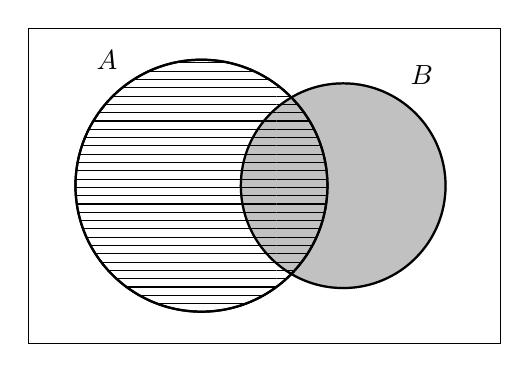
\begin{tikzpicture}
  \draw(0,0) rectangle (6,4);
  \draw(1,3.6) node{$A$};
  \draw(5,3.4) node{$B$};
  \draw[thick,fill=black!80,opacity=0.3](4,2) circle(1.3cm);
  \draw[thick,pattern=horizontal lines](2.2,2) circle(1.6cm);
  \draw[thick](2.2,2) circle(1.6cm);
  \draw[thick](4,2) circle(1.3cm);
\end{tikzpicture}
\end{center}
\caption{A Venn diagram illustrating the definition of conditional probability.
$\Prob(A \mid B)$ is the ratio of the area of the football shaped region that is both
shaded and striped ($A \intersect B$) to the area of the shaded circle ($B$).
}
\label{fig:VennConditional}
\end{figure}

%The example above indicates how we should define conditional probability 
%generally.

%\todo{Venn Diagram}

\begin{boxedText}
%\begin{definition}[Conditional Probability]
  \label{def:condProb}%
  \myindex{conditional probability|defidx}%
  Let $A$ and $B$ be two events such that $\Prob(B) \neq 0$.  
  The \textbf{conditional probability} of $A$ given $B$ is defined by
  \[
  \Prob(A \mid B) = \frac{\Prob(A \intersect B) }{ \Prob(B) }
  \; .
  \]
  If $\Prob(B) = 0$, then $\Prob(A \mid B)$ is undefined.
%  \qed
\end{boxedText}

\begin{example}
  A class of $5$th graders was asked what color should be used for the class
  T-shirt, red or purple. 
  The table below contains a summary of the students' responses:

  \begin{center}
	\medskip
	\begin{tabular}{|l||r|r|}
	  \hline
  & \multicolumn{2}{c|}{Color}\\ 
          & Red & Purple \\ \hline \hline
	Girls & $7$    & $9$ \\ \hline
	Boys  & $10$   & $8$ \\ \hline
  \end{tabular}
  \medskip
\end{center}

  \question Suppose we randomly select a student from this class.
  Let $R$ be the event that a child prefers a red T-shirt.
  Let $B$ be the event that the child is a boy, and let $G$ be 
  the event that the child is a girl.  
  Express each of the following probabilities in words and 
  determine their values:
  \begin{multicols}{3}
  \begin{itemize}
	\item
	  $\Prob(R)$,
	\item
	  $\Prob(R \mid B)$,
	\item
	  $\Prob(B \mid R)$,
	\item
	  $\Prob(R \mid G)$,
	\item
	  $\Prob(G \mid R)$,
	\item
	  $\Prob(B \mid G)$.
  \end{itemize}
  \end{multicols}

  \answer 
  The conditional probabilities can be computed in two ways.  We can use the
  formula from the definition of conditional probability directly,
  or we can consider the condition event to be a new, smaller sample space
  and read the conditional probability from the table.
  \begin{itemize}
	\item
	  $\Prob(R) = 17/34 = 1/2$ because $17$ of the $34$ kids prefer red

	  This is the probability that a randomly selected student prefers red
	\item
	  $\displaystyle \Prob(R \mid B) = \frac{10/34}{18/34} = \frac{10}{18}$ 
	  because $10$ of the $18$ boys prefer red

	  This is the probability that a randomly selected boy prefers red
	\item
	  $\displaystyle \Prob(B \mid R)= \frac{10/34}{17/34} = \frac{10}{17}$ 
	  because $10$ of the $17$ students who prefer red are boys.

	  This is the probability that a randomly selected student who
	  prefers red is a boy.
	\item
	  $\displaystyle \Prob(R \mid G) = \frac{7/34}{16/34} = \frac{7}{16}$ 
	  because $7$ of the $16$ girls prefer red

	  This is the probability that a randomly selected girl prefers red

	\item
	  $\displaystyle \Prob(G \mid R) = \frac{7/34}{17/34} = \frac{7}{17}$ 
	  because $7$ of the $17$ kids who prefer red are girls.

	  This is the probability that a randomly selected kid who prefers red
	  is a girl.

	\item
	  $\displaystyle \Prob(B \mid G) = \frac{0}{16/34} = 0 $ because none of
	  the girls are boys.

	  This is the probability that a randomly selected girl is a boy.
%	  \qedskip
  \end{itemize}
\end{example}

One important use of conditional probability is as a tool to calculate the 
probability of an intersection.

\bigskip  %improve page break

\begin{boxedText}
  \label{lem:probOfInt}
  Let $A$ and $B$ be events with non-zero probability.  Then 
  \begin{align*}
  \Prob(A \intersect B) & =  \Prob(A) \cdot \Prob(B \mid A) \\
  	& =  \Prob(B) \cdot \Prob(A \mid B)  \;.
\end{align*}

  This follows directly from the definition of conditional probability by
  a little bit of algebra and can be generalized to more than two events.
\end{boxedText}

\begin{example}
  \question
  \myindex{dice|exampleidx}%
  If you roll two standard dice, what is the probability of doubles?
  (Doubles is when the two numbers match.)

  \answer
  Let $A$ be the event that we get a number between $1$ and $6$ on the first die.
  So $\Prob(A) = 1$.  Let $B$ be the event that the second number matches
  the first.  Then the probability of doubles is 
  $\Prob(A \intersect B) = \Prob(A) \cdot \Prob(B \mid A) = 1 \cdot \frac16 = \frac16$
  since regardless of what is rolled on the first die, $1$ of the $6$ possibilities 
  for the second die will match it.
\end{example}


\bigskip % improve page break

\begin{example}
  \myindex{cards|exampleidx}%
  \question
  A $5$-card hand is dealt from a standard $52$-card deck.
  What is the probability of getting a flush (all cards the same suit)?

  \answer
  Imagine dealing the cards in order.
  Let $A_i$ be the event that the $i$th card is the same suit as all
  previous cards.
  Then 
  \begin{eqnarray*}
\evProb{flush} & = & \Prob(A_1 
  \intersect  A_2
  \intersect  A_3
  \intersect  A_4
  \intersect  A_5) \\
  & = &  \Prob(A_1) 
  	\cdot \Prob(A_2 \mid A_1)
  	\cdot \Prob(A_3 \mid A_1 \intersect A_2)
  	\cdot \Prob(A_4 \mid A_1 \intersect A_2 \intersect A_3)
	\\ & &
  	\cdot \Prob(A_5 \mid A_1 \intersect A_2 \intersect A_3 \intersect A_4) \\
	& = & 1 \cdot \frac{12}{51} \cdot \frac{11}{50} \cdot \frac{10}{49} 
	\cdot \frac{9}{48} \; 
\end{eqnarray*}
%\otherqedskip
\end{example}

\begin{example}
\newcommand*\redheart{\Large \ensuremath{{\color{red!80!white}\heartsuit}}}
\newcommand*\blueheart{\Large \ensuremath{{\color{blue!80!black}\varheartsuit}}}
	\question
	In a bowl are 4 red Valentine hearts and 2 blue Valentine hearts.  

	If you reach in
	without looking and select two of the Valentines, let $X$ be the number of blue
	Valentines.  Fill in the following probability table.

	\begin{center}
		\begin{tabular}{|l|c|c|c|}
			\hline
			value of $X$ & \qquad 0 \ \qquad & \qquad 1 \ \qquad & \qquad 2 \ \qquad  
			\\
			\hline
			probability & & & 
			\\
			\hline
		\end{tabular}
	\end{center}

	\answer
$\Prob(X=2) 
	= \Prob(\mbox{first is blue} \tand \mbox{second is blue})
	= \Prob(\mbox{first is blue}) \cdot \Prob( \mbox{second is blue} \mid \mbox{first is blue})
	= \frac26 \cdot \frac15 = \frac{2}{30}
$.
Similarly $\Prob(X=0) 
	= \Prob(\mbox{first is red} \tand \mbox{second is red})
	= \Prob(\mbox{first is red}) \cdot \Prob( \mbox{second is red} \mid \mbox{first is red})
	= \frac46 \cdot \frac35 = \frac{12}{30}
$
Finally, $\Prob(X=1) = 1 - \Prob(X=0) - \Prob(X=2) = 1 - \frac{14}{30} = \frac{16}{30}$

We can represent this using a \term{tree diagram} as well.

\begin{center}
	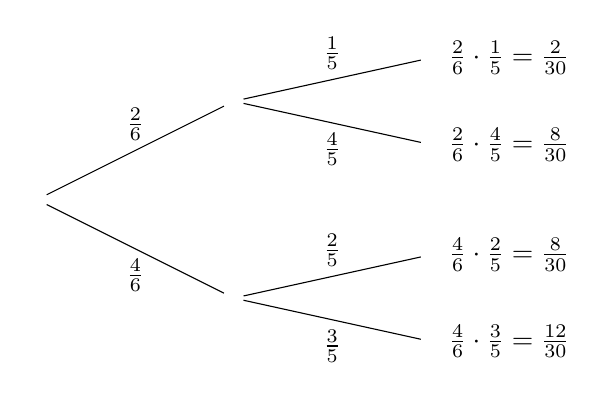
\begin{tikzpicture}
		[level 1/.style={sibling distance=25mm},
		 level 2/.style={sibling distance=11mm},
		 level distance=25mm] 
			\node {} [grow'=right]
			child {node {\blueheart} 
				child {node (bb) {\blueheart} edge from parent node[above]{$\frac15$}} 
				child {node (br) {\redheart}  edge from parent  node[below]{$\frac45$}} 
				edge from parent node[above]{$\frac26$} 
				}
			child {node {\redheart}  
				child {node (rb) {\blueheart} edge from parent  node[above]{$\frac25$}} 
				child {node (rr) {\redheart}  edge from parent  node[below]{$\frac35$}} 
				edge from parent node[below]{$\frac46$} 
			} ; 
			\node [right of=bb] {$\frac26 \cdot \frac15 = \frac{2}{30}$};
			\node [right of=br] {$\frac26 \cdot \frac45 = \frac{8}{30}$};
			\node [right of=rb] {$\frac46 \cdot \frac25 = \frac{8}{30}$};
			\node [right of=rr] {$\frac46 \cdot \frac35 = \frac{12}{30}$};
	\end{tikzpicture}
\end{center}
The edges in the tree represent conditional probabilities which we can multiply together
to the probability that all events on a particular branch happen.  The first level of branching 
represents what kind of Valentine is selected first, the second level represents the 
second selection.
	
\end{example}

\newpage

\begin{example}
  \label{example:sensitivitySpecificity}%
  \question
  Suppose a test correctly 
%  \myindex{sensitivity|exampleidx}%
%  \myindex{specificity|exampleidx}%
  \myindex{medical testing|exampleidx}%
  identifies diseased people $99$\% of the time and correctly
  identifies healthy people $98$\% of the time.  
  Furthermore assume that in a certain population,
  one person in $1000$ has the disease.  
  If a random person is tested and the test comes back positive, 
  what is the probability that the person has the disease?

  \answer
  We begin by introducing some notation.  Let $D$ be the event that
  a person has the disease.  Let $H$ be the event that the person is
  healthy.  Let $+$ be the event that the test comes back positive (meaning 
  it indicates disease -- probably a negative from the perspective 
  of the person tested).  Let $-$ be the event that the test is negative.
	\begin{itemize}
	  \item $\Prob(D) = 0.001$, so $\Prob(H) = 0.999$.

	  \item $\Prob(+ \mid D) = 0.99$, so 
	  $\Prob(- \mid D) = 0.01$.

		$\Prob(+ \mid D)$ is called the \term{sensitivity} of the test.
		(It tells how sensitive the test is to the presence of the disease.)
	  \item 
		$\Prob(-\mid H) = 0.98$, so $\Prob(+\mid H) = 0.02$.
		\medskip

	  $\Prob(- \mid H)$ is called the \term{specificity} of the test.
		\smallskip

	  \item $\!\!\!\!\!$
	  \begin{tabular}[t]{rcl}
	  $\ds \Prob(D \mid +) $
		&$\!=\!$& $\displaystyle \frac{\Prob(D \intersect +)}{\Prob(+)}$
		\\[5mm]
		&$\; = \;$& 
		$\displaystyle \frac{\Prob(D) \cdot \Prob(+ \mid D)}{\Prob(D \intersect +) 
			+ \Prob(H \intersect +)  }$
			\\[5mm]
			& $\!=\!$ & $\displaystyle 
				\frac{0.001 \cdot 0.99}{0.001 \cdot 0.99 + 0.999 \cdot 0.02}
		            \; = \;  0.0472$. 
		\end{tabular}
	  \end{itemize}
	  A tree diagram is a useful way to visualize these calculations.
\begin{center}
	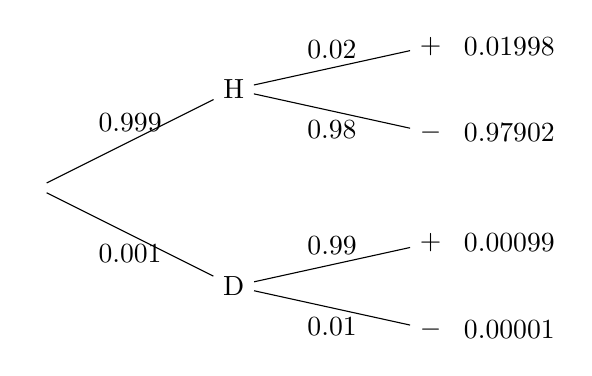
\begin{tikzpicture}
		[level 1/.style={sibling distance=25mm},
		 level 2/.style={sibling distance=11mm},
		 level distance=25mm] 
			\node {} [grow'=right]
			child {node {H} 
				child {node (bb) {$+$} edge from parent node[above]{$0.02$}} 
				child {node (br) {$-$}  edge from parent  node[below]{$0.98$}} 
				edge from parent node[above]{$0.999$} 
				}
			child {node {D}  
				child {node (rb) {$+$} edge from parent  node[above]{$0.99$}} 
				child {node (rr) {$-$}  edge from parent  node[below]{$0.01$}} 
				edge from parent node[below]{$0.001$} 
			} ; 
			\node [right of=bb] {0.01998 };
			\node [right of=br] {0.97902 };
			\node [right of=rb] {0.00099 };
			\node [right of=rr] {0.00001 };
	\end{tikzpicture}
\end{center}

	  This low probability surprises most people the first time they see it.
	  This means that if the test result of a random person comes back positive,
	  the probability that that person has the disease is less than $5$\%, 
	  even though the test is ``highly accurate''.   
	  This is one reason why we do not routinely 
	  screen an entire population for a rare disease -- such screening would 
	  produce many more false positives than true positives.

	  Of course, if a doctor orders a test, it is usually because there 
	  are some other symptoms.  This changes the \emph{a priori} probability
	  that the patient has the disease.  
%	  Exercise~\ref{prob:bayesDisease}
%	  gives you a chance to explore this further.
\end{example}

\newpage

\subsection{Independence}

\begin{boxedText}
  \label{def:independentEvents}%
  \myindex{independent events|defidx}%
  Let $A$ and $B$ be two events such that $\Prob(B) = \Prob(B \mid A)$.
  Such events are called \term{independent}.
\end{boxedText}

When events are independent, then 
$\Prob(A \tand B) = \Prob(A) \cdot \Prob(B \mid A) = \Prob(A) \cdot \Prob(B)$.
This makes probability calculations much simpler -- but it only applies
for independent events.

\begin{example}
	\question 
	What is the probability of rolling double sixes with standard 6-sided dice?

	\answer
	Let $A$ be the event that the first die is a 6 and let $B$ be the event that the 
	second die is a 6.  Since $A$ and $B$ are independent, 
	$\Prob(A \tand B) = \Prob(A) \cdot \Prob(B) = \frac16 \cdot \frac16 = \frac{1}{36}$.
\end{example}

\begin{example}
	\question What is the probability of flipping a coin five times and getting 5 heads?

	\answer  Since each coin toss is independent of the others, the probability
	of getting five heads is the product of the probabilities of each coin coming up
	heads:

	\[ 
	\Prob(\mbox{5 heads in 5 flips}) = (0.5)^5 = 0.03125 
	\]

	
\end{example}

\begin{example}
	\question
	A manufacturer claims that 99\% of its parts will still be functioning properly 
	two years after purchase.  If you purchase 10 of these parts, what is the probability
	that all 10 of them are still functioning properly two years later (assuming the
	manufacturer's claim is correct)?

	\answer
	Let $G_i$ be the event that part $i$ is still functioning properly after two years.
	We want to calculate 
	\[
	\Prob(G_1 \tand G_2 \tand \cdots \tand G_{10})\;.
	\]
	If we assume the lifetimes of the parts are independent, then 
	\[
	\Prob(G_1 \tand G_2 \tand \cdots \tand G_{10})
	=
	\underbrace{.99 \cdot .99 \cdot .99 \cdots .99 = .99^{10}}_{\mbox{10 of these}}
	= 0.9043821\;.
	\]

	The independence assumption may or may not be valid.  That depends on the manufacturing
	process.  For example, if the primary way a part goes bad is that the package 
	is dropped during shipping, then if you by a box of 10 and the first part is bad, 
	they will all be bad.  And if the box was handled carefully and never dropped, and the first part used is good, they will likely all be good.  So in
	that extreme case, the probability that all 10 are functioning properly after two years
	is 99\%.



\end{example}

\newpage
\section*{Exercises}

\begin{problem}
	Amy is a 92\% free throw shooter.  If she shoots
	100 free throws after practice, what is the probability that she
	makes at least 95 of them?  Use simulation to estimate this probability.

	(You can use \function{rflip()} to simulate shooting free throws.
	The \option{prob} argument lets you set the probability.  In this case,
	you need to set it to $0.92$.  Then think of a head as a made free throw
	and a tail as a missed free throw.)
\end{problem}

\begin{solution}
\begin{knitrout}
\definecolor{shadecolor}{rgb}{0.969, 0.969, 0.969}\color{fgcolor}\begin{kframe}
\begin{alltt}
\hlkwd{set.seed}\hlstd{(}\hlnum{123}\hlstd{)}  \hlcom{# so we get the same simulated results each time we compile.}
\hlstd{sims} \hlkwb{<-} \hlkwd{do}\hlstd{(}\hlnum{1000}\hlstd{)} \hlopt{*} \hlkwd{rflip}\hlstd{(}\hlnum{100}\hlstd{,} \hlkwc{prob} \hlstd{=} \hlnum{0.92}\hlstd{)}
\hlkwd{tally}\hlstd{(}\hlopt{~}\hlstd{heads} \hlopt{>} \hlnum{95}\hlstd{,} \hlkwc{data} \hlstd{= sims)}
\end{alltt}
\begin{verbatim}
## 
##  TRUE FALSE 
##    94   906
\end{verbatim}
\end{kframe}
\end{knitrout}
So the probability that Amy makes more than 95 shots in 100 attempts is approximately
0.094
\end{solution}

\begin{problem}
	\begin{enumerate}
		\item
	Use simulation to estimate the probability of rolling a difference of 2 when rolling
	two fair six-sided dice.
\item
	Make a histogram showing the results for all of the possible differences.
	\end{enumerate}

\end{problem}

\begin{solution}
\begin{knitrout}
\definecolor{shadecolor}{rgb}{0.969, 0.969, 0.969}\color{fgcolor}\begin{kframe}
\begin{alltt}
\hlstd{d} \hlkwb{<-} \hlstd{die1} \hlopt{-} \hlstd{die2}
\hlkwd{tally}\hlstd{(}\hlopt{~}\hlstd{d)}
\end{alltt}
\begin{verbatim}
## 
##   -5   -4   -3   -2   -1    0    1    2    3    4    5 
##  285  528  845 1108 1413 1652 1355 1098  823  587  306
\end{verbatim}
\begin{alltt}
\hlkwd{prop}\hlstd{(}\hlopt{~}\hlstd{(d} \hlopt{==} \hlnum{8}\hlstd{))}
\end{alltt}
\begin{verbatim}
## TRUE 
##    0
\end{verbatim}
\begin{alltt}
\hlkwd{histogram}\hlstd{(}\hlopt{~}\hlstd{d,} \hlkwc{width} \hlstd{=} \hlnum{1}\hlstd{)}  \hlcom{# setting width is important for integer data}
\end{alltt}
\end{kframe}

{\centering \includegraphics[width=\maxwidth]{figures/fig-unnamed-chunk-9-1} 

}



\end{knitrout}
\end{solution}

\begin{problem}
	Use simulation to estimate the probability that when dealing 
	5 cards from a standard (well-shuffled) deck of 52 cards
	all five are diamonds.  

	You can simulate the deck of cards using the numbers 1 through 52 and consider the numbers
	1 through 13 to be the diamonds.  Instead of using \function{resample()}, which would allow
	you to get the same card more than once, we need to use \function{sample()}, which does not.
	(You can also use \function{deal()} which does the same thing.)
\begin{knitrout}
\definecolor{shadecolor}{rgb}{0.969, 0.969, 0.969}\color{fgcolor}\begin{kframe}
\begin{alltt}
\hlkwd{sample}\hlstd{(}\hlnum{1}\hlopt{:}\hlnum{52}\hlstd{,} \hlnum{5}\hlstd{)}
\end{alltt}
\begin{verbatim}
## [1] 19 26 36 30 21
\end{verbatim}
\begin{alltt}
\hlkwd{sample}\hlstd{(}\hlnum{1}\hlopt{:}\hlnum{52}\hlstd{,} \hlnum{5}\hlstd{)}
\end{alltt}
\begin{verbatim}
## [1] 52 10 21 28 12
\end{verbatim}
\begin{alltt}
\hlkwd{deal}\hlstd{(}\hlnum{1}\hlopt{:}\hlnum{52}\hlstd{,} \hlnum{5}\hlstd{)}
\end{alltt}
\begin{verbatim}
## [1] 19  8 52 51 18
\end{verbatim}
\begin{alltt}
\hlkwd{deal}\hlstd{(}\hlnum{1}\hlopt{:}\hlnum{52}\hlstd{,} \hlnum{5}\hlstd{)}
\end{alltt}
\begin{verbatim}
## [1] 30 23 20 51 15
\end{verbatim}
\end{kframe}
\end{knitrout}
	There is another way to make the calculation, using the function \function{sum}. \R\ can tell you how many cards are below 14 using \function{sum} because \R\ turns TRUE into 1
	and FALSE into 0 when you do a sum.
\begin{knitrout}
\definecolor{shadecolor}{rgb}{0.969, 0.969, 0.969}\color{fgcolor}\begin{kframe}
\begin{alltt}
\hlkwd{sum}\hlstd{(}\hlkwd{sample}\hlstd{(}\hlnum{1}\hlopt{:}\hlnum{52}\hlstd{,} \hlnum{5}\hlstd{)} \hlopt{<} \hlnum{14}\hlstd{)}
\end{alltt}
\begin{verbatim}
## [1] 1
\end{verbatim}
\begin{alltt}
\hlkwd{sum}\hlstd{(}\hlkwd{sample}\hlstd{(}\hlnum{1}\hlopt{:}\hlnum{52}\hlstd{,} \hlnum{5}\hlstd{)} \hlopt{<} \hlnum{14}\hlstd{)}
\end{alltt}
\begin{verbatim}
## [1] 1
\end{verbatim}
\begin{alltt}
\hlkwd{sum}\hlstd{(}\hlkwd{sample}\hlstd{(}\hlnum{1}\hlopt{:}\hlnum{52}\hlstd{,} \hlnum{5}\hlstd{)} \hlopt{<} \hlnum{14}\hlstd{)}
\end{alltt}
\begin{verbatim}
## [1] 2
\end{verbatim}
\end{kframe}
\end{knitrout}
	You can use \function{do()} to do this many times. (Three is \emph{not} many\! We just do a small number here 
	for illustration purposes.)
\begin{knitrout}
\definecolor{shadecolor}{rgb}{0.969, 0.969, 0.969}\color{fgcolor}\begin{kframe}
\begin{alltt}
\hlkwd{do}\hlstd{(}\hlnum{3}\hlstd{)} \hlopt{*} \hlkwd{sum}\hlstd{(}\hlkwd{sample}\hlstd{(}\hlnum{1}\hlopt{:}\hlnum{52}\hlstd{,} \hlnum{5}\hlstd{)} \hlopt{<} \hlnum{14}\hlstd{)}
\end{alltt}
\begin{verbatim}
##   sum
## 1   0
## 2   1
## 3   1
\end{verbatim}
\end{kframe}
\end{knitrout}
\end{problem}

\begin{solution}
\begin{knitrout}
\definecolor{shadecolor}{rgb}{0.969, 0.969, 0.969}\color{fgcolor}\begin{kframe}
\begin{alltt}
\hlkwd{tally}\hlstd{(}\hlopt{~}\hlstd{result,} \hlkwd{do}\hlstd{(}\hlnum{10000}\hlstd{)} \hlopt{*} \hlkwd{sum}\hlstd{(}\hlkwd{sample}\hlstd{(}\hlnum{1}\hlopt{:}\hlnum{52}\hlstd{,} \hlnum{5}\hlstd{)} \hlopt{<} \hlnum{14}\hlstd{))}
\end{alltt}


{\ttfamily\noindent\itshape\color{messagecolor}{\#\# First argument should be a formula... But I'll try to guess what you meant}}

{\ttfamily\noindent\bfseries\color{errorcolor}{\#\# Error in as.data.frame.default(x[[i]], optional = TRUE): cannot coerce class "{}"{}formula"{}"{} to a data.frame}}\end{kframe}
\end{knitrout}
\end{solution}

\begin{problem}
Parts in a manufacturing plant go through two quality control checks before they
are shipped.  99\% of parts pass inspection A and 98\% parts pass inspection B.
0.5\% fail both inspections.  

What percentage of parts pass both inspections?
\end{problem}

\begin{solution}
	$\Prob(\mbox{fail at least one}) = \Prob(\mbox{fail A or fail B}) =
	\Prob(\mbox{fail A}) + \Prob(\mbox{fail B}) - \Prob(\mbox{fail both})
	= 0.01 + 0.02 - 0.05 = 0.025$.

	So $\Prob(\mbox{pass both}) = 1 - 0.025 = 0.975$.
\end{solution}

\begin{problem} 
	Let $X$ be the sum of the results of rolling two fair six-sided dice.
	\begin{enumerate}
		\item
			What is $\Prob(\mbox{$X$ is even and $X < 5$})$?
		\item
			What is $\Prob(\mbox{$X$ is even or $X < 5$})$? 
	\end{enumerate}
\end{problem}

\begin{solution}
	$\Prob(\mbox{$X$ is even and $X < 5$}) 
	= \Prob(X = 2 \tor X=4) = 1/36 + 3/36 = 4/36 = 0.0833333$

$\Prob(\mbox{$X$ is even or $X < 5$}) = \Prob(\mbox{$X$ is even}) + \Prob(X=3)
= 18/36 + 2/36 = 20/36 = 0.5555556$.
\end{solution}

\begin{problem}
Let $Y$ be the difference between the larger and smaller number when two fair dice 
are rolled.  (So if you roll a 2 and a 4, then the value of $Y$ is 2.)  
\begin{enumerate}
	\item 
		What is $\Prob(Y=2)$?
	\item
		What are the other possible values of $Y$?
	\item 
		Calculate the probability for each possible value of $Y$
		and put those values in a table.
\end{enumerate}
\end{problem}

\begin{solution}
	$Y = 2$ for rolls of $(3,1)$, $(4,2)$, $(5,3)$, and $(6,4)$.  Each of these 
	can also happen in the other order, so the probability is $8/36 = 2/9 = 0.2222222$.

\begin{center}
	\begin{tabular}{lrrrrrr}
		\hline
		value of $Y$ & 0 & 1 & 2 & 3 & 4 & 5 \\
		\hline
		probability & 6/36 & 10/36 & 8/36 & 6/36 & 4/36 & 2/36 \\
		\hline
	\end{tabular}
\end{center}
\begin{knitrout}
\definecolor{shadecolor}{rgb}{0.969, 0.969, 0.969}\color{fgcolor}\begin{kframe}
\begin{alltt}
\hlkwd{c}\hlstd{(}\hlnum{6}\hlstd{,} \hlnum{10}\hlstd{,} \hlnum{8}\hlstd{,} \hlnum{6}\hlstd{,} \hlnum{4}\hlstd{,} \hlnum{2}\hlstd{)}\hlopt{/}\hlnum{36}
\end{alltt}
\begin{verbatim}
## [1] 0.16666667 0.27777778 0.22222222 0.16666667 0.11111111 0.05555556
\end{verbatim}
\end{kframe}
\end{knitrout}
\end{solution}

\begin{problem}
	A device is assembled from two primary parts.  2\% of the first type of part
	are defective and 3\% of the other type of part are defective.  The device
	only functions properly if both parts are functioning properly.
	\begin{enumerate}
	\item
	What assumption do you need to make to calculate the probability
	that a device assembled in this way will function properly?
	Is it a reasonable assumption in this situation?  Explain.
	\item
	What is the probability that that a device assembled in this way will 
	function properly?
	\end{enumerate}
\end{problem}

\begin{solution}
	Assuming failure of each part is independent of failure of the other,
	the probability that both function properly is 
	$0.98 \cdot 0.97 = 0.9506$.
\end{solution}

\begin{problem}
According to the CDC, ``Compared to nonsmokers, men who smoke are about 23
times more likely to develop lung cancer and women who smoke are about 13 times
more likely.''  According to the American Lung Association: 
``In 2008, 21.1 million (18.3\%) women smoked in the United States 
compared to 24.8 million (23.1\%) men.''

\begin{enumerate}
	\item
		If you learn that a person is a smoker and no nothing else 
		about the person, what is the probability that the person is a woman?
	\item
		If you learn that a woman has been diagnosed with lung cancer,
		and you know nothing else about her, what is the probability that she is a
		smoker?
	\item
		If you learn that a man has been diagnosed with lung cancer,
		and you know nothing else about him, what is the probability that he is a
		smoker?
\end{enumerate}
\end{problem}

\begin{solution}
\begin{knitrout}
\definecolor{shadecolor}{rgb}{0.969, 0.969, 0.969}\color{fgcolor}\begin{kframe}
\begin{alltt}
\hlcom{# a)}
\hlnum{21.1}\hlopt{/}\hlstd{(}\hlnum{21.1} \hlopt{+} \hlnum{24.8}\hlstd{)}
\end{alltt}
\begin{verbatim}
## [1] 0.459695
\end{verbatim}
\end{kframe}
\end{knitrout}
Part b is the most interesting (once you can do that, you can do part c the same way).
Let $W$ be the event that someone is a woman, $S$ that they are a smoker, and $C$ that they
get cancer. Let $x = \Prob( C | W \intersect S^c)$.  Then $\Prob( C | W \intersect S ) = 13x$.

\begin{align*}
	\Prob( S | W \intersect C ) 
	& = \frac{ \Prob(S \intersect W \intersect C) }{\Prob(W \intersect C)}
	\\
	& = \frac{ \Prob(S \intersect W \intersect C) }
	{\Prob(S \intersect W \intersect C) + \Prob( S^c \intersect W \intersect C)}
\end{align*}
So we just need to compute the two probabilities in the denominator.
\begin{align*}
	\Prob(S \intersect W \intersect C)
	&= \Prob(W) \cdot \Prob(S \mid W) \cdot \Prob(C \mid W \intersect S) 
	\\
	&= \Prob(W) \cdot 0.183 \cdot 13x
	\\
	\Prob(S^c \intersect W \intersect C)
	&= \Prob(W) \cdot \Prob(S^c \mid W) \cdot \Prob(C \mid W \intersect S^c) 
	\\
	&= \Prob(W) \cdot 0.817 \cdot x
\end{align*}
After factoring out $x \cdot \Prob(W)$, the arithmetic is now easy:

\begin{knitrout}
\definecolor{shadecolor}{rgb}{0.969, 0.969, 0.969}\color{fgcolor}\begin{kframe}
\begin{alltt}
\hlcom{# b) After factoring out a constant from numerator and denominator we are left with}
\hlnum{0.183} \hlopt{*} \hlnum{13}\hlopt{/}\hlstd{(}\hlnum{0.183} \hlopt{*} \hlnum{13} \hlopt{+} \hlnum{0.817} \hlopt{*} \hlnum{1}\hlstd{)}
\end{alltt}
\begin{verbatim}
## [1] 0.744368
\end{verbatim}
\begin{alltt}
\hlcom{# c) After factoring out a constant from numerator and denominator we are left with}
\hlnum{0.231} \hlopt{*} \hlnum{23}\hlopt{/}\hlstd{(}\hlnum{0.231} \hlopt{*} \hlnum{23} \hlopt{+} \hlnum{0.769} \hlopt{*} \hlnum{1}\hlstd{)}
\end{alltt}
\begin{verbatim}
## [1] 0.8735613
\end{verbatim}
\end{kframe}
\end{knitrout}

Note: Another approach to part b is to consider the sample space to be only the women.
If you do it that way, you can avoid mentioning any probabilities involving $W$.  (In the end, 
they factor out anyway.)  Of course, you can do a similar thing for the men.
\end{solution}

\begin{problem}
A manufacturing plant has kept records that show that the number of parts produced each 
day and on the proportion of parts that are defective.

\begin{center}
\begin{tabular}{|lrrrr|}
	\hline
	& Monday & Tuesday & Wednesday & Thursday \\
	\hline
	Proportion of weekly production & 20\% & 25\% & 28\% & 27\%  
	\\
	Rate of defective parts & 2\% & 1.5\% & 1\%  & 3\% 
	\\
	\hline
\end{tabular}
\end{center}
\begin{enumerate}
	\item
		If you order a part from this company, what is the probability that it was produced
		on a Monday or a Thursday?
\item
If you order a part from this company and it is defective, 
what is the probability that it was produced on a Monday or a Thursday?
\item
	If you order a part from this company and it functions properly, 
	what is the probability that it was produced on a Monday or Thursday?
\end{enumerate}
Express your answers to 3 significant digits and avoid internal rounding.

\end{problem}

\begin{solution}
You may find a tree diagram useful here to visualize these probabilities.
\begin{knitrout}
\definecolor{shadecolor}{rgb}{0.969, 0.969, 0.969}\color{fgcolor}\begin{kframe}
\begin{alltt}
\hlcom{# part a}
\hlnum{.20} \hlopt{+} \hlnum{.27}
\end{alltt}
\begin{verbatim}
## [1] 0.47
\end{verbatim}
\begin{alltt}
\hlcom{# part b: P( Wed-Thur | defective ) = P( Wed-Thur and defective ) / P(defective)}
\hlstd{a} \hlkwb{<-} \hlnum{.20} \hlopt{*} \hlnum{.02} \hlopt{+}       \hlcom{# Monday and defective}
     \hlnum{.27} \hlopt{*} \hlnum{.03}         \hlcom{# Thursday and defective}
\hlstd{b} \hlkwb{<-} \hlnum{.25} \hlopt{*} \hlnum{.015} \hlopt{+}      \hlcom{# Tuesday and defective}
     \hlnum{.28} \hlopt{*} \hlnum{.01}         \hlcom{# Wednesday and defective }
\hlstd{a} \hlopt{/} \hlstd{(a} \hlopt{+} \hlstd{b)}
\end{alltt}
\begin{verbatim}
## [1] 0.6487936
\end{verbatim}
\begin{alltt}
\hlcom{# part c: P( Wed-Thur | good ) = P( Wed-Thur and good ) / P(good)}
\hlstd{c} \hlkwb{<-} \hlnum{.20} \hlopt{*} \hlnum{.98} \hlopt{+}       \hlcom{# Monday and good}
     \hlnum{.27} \hlopt{*} \hlnum{.97}         \hlcom{# Thursday and good}
\hlstd{d} \hlkwb{<-} \hlnum{.25} \hlopt{*} \hlnum{.985} \hlopt{+}      \hlcom{# Tuesday and good}
     \hlnum{.28} \hlopt{*} \hlnum{.99}         \hlcom{# Wednesday and good }
\hlstd{c} \hlopt{/} \hlstd{(c} \hlopt{+} \hlstd{d)}
\end{alltt}
\begin{verbatim}
## [1] 0.4666021
\end{verbatim}
\end{kframe}
\end{knitrout}
\end{solution}


\shipoutProblems

\vfill

\begin{center}
	\includegraphics[width=.4\textwidth]{images/cigarettes-cartoon}
\end{center}

\ifsolutions
\ifsolutionslocal
\newpage
\section*{Solutions}
\shipoutSolutions
\fi
\fi
 



\chapter{Densities}

\section{Density histograms, density plots, density functions}
\myindex{density|defidx}%
A histogram is a simple picture describing the ``density" of data. 
Histogram bars are tall in regions where there is more data -- i.e., where the data are 
more ``dense''.  
\begin{knitrout}
\definecolor{shadecolor}{rgb}{0.969, 0.969, 0.969}\color{fgcolor}\begin{kframe}
\begin{alltt}
\hlkwd{require}\hlstd{(alr3)}
\hlkwd{histogram}\hlstd{(}\hlopt{~}\hlstd{Duration,} \hlkwc{data} \hlstd{= oldfaith)}
\hlkwd{histogram}\hlstd{(}\hlopt{~}\hlstd{Duration,} \hlkwc{data} \hlstd{= oldfaith,} \hlkwc{type} \hlstd{=} \hlstr{"count"}\hlstd{)}
\end{alltt}
\end{kframe}

{\centering \includegraphics[width=\maxwidth]{figures/fig-histograms-count-density-1} 
\includegraphics[width=\maxwidth]{figures/fig-histograms-count-density-2} 

}



\end{knitrout}

The density scale is the same scale that is used by \function{densityplot()}, and it
is the default scale for histograms created using \function{histogram()} when
the \pkg{mosaic} package is loaded.
\begin{knitrout}
\definecolor{shadecolor}{rgb}{0.969, 0.969, 0.969}\color{fgcolor}\begin{kframe}
\begin{alltt}
\hlkwd{require}\hlstd{(alr3)}
\hlkwd{histogram}\hlstd{(}\hlopt{~}\hlstd{Duration,} \hlkwc{data} \hlstd{= oldfaith,} \hlkwc{width} \hlstd{=} \hlnum{20}\hlstd{,} \hlkwc{center} \hlstd{=} \hlnum{110}\hlstd{)}
\hlkwd{densityplot}\hlstd{(}\hlopt{~}\hlstd{Duration,} \hlkwc{data} \hlstd{= oldfaith)}
\end{alltt}
\end{kframe}

{\centering \includegraphics[width=\maxwidth]{figures/fig-histogram-density-1} 
\includegraphics[width=\maxwidth]{figures/fig-histogram-density-2} 

}



\end{knitrout}

The density scale is chosen so that the area of each rectangular bar (width times height)
is equal to the proportion of the data set represented by the rectangle. 

\begin{example}
	\question Use the histogram of Old Faithful eruption times to estimate
	the proportion of eruptions that last between 100 and 120 seconds.

	\answer
In our histogram of Old Faithful eruption durations, the bar corresponding to the 
bin from 100--120 appears to have a height of about 0.09.  That gives an area of 
0.18 and indicates that approximately 18\% of the eruptions last between 100 and 120
seconds.
\begin{knitrout}
\definecolor{shadecolor}{rgb}{0.969, 0.969, 0.969}\color{fgcolor}\begin{kframe}
\begin{alltt}
\hlkwd{tally}\hlstd{(}\hlopt{~}\hlstd{(}\hlnum{100} \hlopt{<} \hlstd{Duration} \hlopt{&} \hlstd{Duration} \hlopt{<=} \hlnum{120}\hlstd{),} \hlkwc{data} \hlstd{= oldfaith,} \hlkwc{format} \hlstd{=} \hlstr{"prop"}\hlstd{)}
\end{alltt}
\begin{verbatim}
## 
##      TRUE     FALSE 
## 0.1888889 0.8111111
\end{verbatim}
\end{kframe}
\end{knitrout}
\end{example}

The key idea behind the density scale can be expressed as 

\begin{center}
	Probability $=$ area
\end{center}
This association of area with probability means that
the total area of all the bars will always be equal to 1 if we use the density
scale.  

It also provides us with a way to describe a distribution with a mathematical function.


\begin{boxedText}
  \label{def:pdf}%
  \myindex{probability density function|defidx}%
  \myindex{density function|defidx}%
  \myindex{pdf|see{probability density function}}%
  Let $f$ be a function such that %: \reals \to \reals$ be a function such that
  \begin{enumerate}
	  \item $f(x) \ge 0$ for all $x$,
	  \item $\displaystyle \int_{-\infty}^{\infty} f(x) \; dx = 1$.
   \end{enumerate}
   Then $f$ is called a \textbf{density function} (or probability density function,
   abbreviated pdf) and describes a continuous random variable $X$ such that
   \[
   \Prob(a\le X \le b) = \int_a^b f(x) \; dx \;.
   \]
\end{boxedText}



\begin{example}
\label{ex:triangle}%
	Let $f$ be defined by
	\[
	f(x) = \begin{cases}  
		1 - |x| & x \in [-1,1] \\
		0 & \mbox{otherwise}\\
	\end{cases}
	\]
Show that $f$ is a density function.  Let $X$ be the associated random 
variable, and compute the following probabilities:
\begin{enumerate}
	\item
		$\Prob(X\le0)$
	\item
		$\Prob(X \le 1)$
	\item
		$\Prob(X \le \frac12)$
	\item
		$\Prob(-\frac12 X \le \frac12)$
\end{enumerate}

\answer
While we could set up integrals for these, it is easier to solve them using geometry.%
\footnote{\R\ cleverly turns TRUE and FALSE into 1 and 0 when you use them in arithmetic
expressions.  The definition of \code{f()} makes use of this conversion to simplify specifying
the cases.}
\begin{knitrout}
\definecolor{shadecolor}{rgb}{0.969, 0.969, 0.969}\color{fgcolor}\begin{kframe}
\begin{alltt}
\hlstd{f} \hlkwb{<-} \hlkwd{makeFun}\hlstd{((}\hlnum{1} \hlopt{-} \hlkwd{abs}\hlstd{(x))} \hlopt{*} \hlstd{(}\hlkwd{abs}\hlstd{(x)} \hlopt{<=} \hlnum{1}\hlstd{)} \hlopt{~} \hlstd{x)}
\hlkwd{plotFun}\hlstd{(}\hlkwd{f}\hlstd{(x)} \hlopt{~} \hlstd{x,} \hlkwc{x.lim} \hlstd{=} \hlkwd{c}\hlstd{(}\hlopt{-}\hlnum{1.5}\hlstd{,} \hlnum{1.5}\hlstd{))}
\end{alltt}
\end{kframe}

{\centering \includegraphics[width=\maxwidth]{figures/fig-unnamed-chunk-19-1} 

}



\end{knitrout}

The entire area under the curve can be found as the area of a triangle with base 2 and height 1.
\[
\int_{-\infty}^{\infty} f(x) \; dx 
=
\int_{-1}^1 f(x) \; dx
=
\frac 12 \cdot 2 \cdot 1 = 1
\]
This implies that $f$ is a density function.

\begin{enumerate}
	\item
$\Prob(X \le 1) 
=
\int_{-\infty}^{1} f(x) \; dx 
=
\int_{-1}^{1} f(x) \; dx = 1
$
\item
		$\Prob(X \le \frac12)
		=
\int_{-\infty}^{1/2} f(x) \; dx 
=
\int_{-1}^{1/2} f(x) \; dx = 1 - \frac12 \cdot \frac12 \cdot \frac12 = \frac78
$

\item
	$\Prob( -\frac12 \le X \le \frac 12 ) 
	=
	\int_{-1/2}^{1/2} f(x) \; dx 
	=
	1 - \frac28 = \frac34
	$
\end{enumerate}

We can also let \R\ do (numerical) integration for us.  There are two ways to do this.
The first method uses the \function{integrate()} function.
\begin{knitrout}
\definecolor{shadecolor}{rgb}{0.969, 0.969, 0.969}\color{fgcolor}\begin{kframe}
\begin{alltt}
\hlkwd{integrate}\hlstd{(f,} \hlopt{-}\hlnum{Inf}\hlstd{,} \hlnum{1}\hlstd{)}
\end{alltt}
\begin{verbatim}
## 1 with absolute error < 9.2e-05
\end{verbatim}
\begin{alltt}
\hlcom{# this will be more accurate since we aren't asking R to approximate something that we}
\hlcom{# already know is exactly 0}
\hlkwd{integrate}\hlstd{(f,} \hlopt{-}\hlnum{1}\hlstd{,} \hlnum{1}\hlstd{)}
\end{alltt}
\begin{verbatim}
## 1 with absolute error < 1.1e-14
\end{verbatim}
\begin{alltt}
\hlkwd{integrate}\hlstd{(f,} \hlopt{-}\hlnum{0.5}\hlstd{,} \hlnum{0.5}\hlstd{)}
\end{alltt}
\begin{verbatim}
## 0.75 with absolute error < 8.3e-15
\end{verbatim}
\begin{alltt}
\hlcom{# if you just want the value without the text saying how accurate the approximation is}
\hlkwd{integrate}\hlstd{(f,} \hlopt{-}\hlnum{0.5}\hlstd{,} \hlnum{0.5}\hlstd{)}\hlopt{$}\hlstd{value}
\end{alltt}
\begin{verbatim}
## [1] 0.75
\end{verbatim}
\end{kframe}
\end{knitrout}

An alternative approach uses \function{antiD()} from the \pkg{mosaic} package.
\begin{knitrout}
\definecolor{shadecolor}{rgb}{0.969, 0.969, 0.969}\color{fgcolor}\begin{kframe}
\begin{alltt}
\hlstd{F} \hlkwb{<-} \hlkwd{antiD}\hlstd{(} \hlkwd{f}\hlstd{(x)} \hlopt{~} \hlstd{x)}
\hlkwd{F}\hlstd{(}\hlnum{1}\hlstd{)} \hlopt{-} \hlkwd{F}\hlstd{(}\hlopt{-}\hlnum{1}\hlstd{)}        \hlcom{# total probability -- better be 1}
\end{alltt}
\begin{verbatim}
## [1] 1
\end{verbatim}
\begin{alltt}
\hlkwd{F}\hlstd{(}\hlnum{.5}\hlstd{)} \hlopt{-} \hlkwd{F}\hlstd{(}\hlopt{-}\hlnum{1}\hlstd{)}       \hlcom{# P( -1 <= X <= 0.5 )}
\end{alltt}
\begin{verbatim}
## [1] 0.875
\end{verbatim}
\begin{alltt}
\hlkwd{F}\hlstd{(}\hlnum{.5}\hlstd{)} \hlopt{-} \hlkwd{F}\hlstd{(}\hlopt{-}\hlnum{.5}\hlstd{)}      \hlcom{# P( -.5 <= X <= .5 )}
\end{alltt}
\begin{verbatim}
## [1] 0.75
\end{verbatim}
\end{kframe}
\end{knitrout}
\end{example}

\myindex{cumulative distribution function|defidx}%
\myindex{cdf|see{cumulative distribution function}}%
If we help \R\ choose the anti-derivative, we get a useful function called 
the \term{cumulative distribution function}, abbreviated cdf.


\begin{boxedText}
	If $X$ is a random variable, then the \term{cumulative distribution function} (cdf) for 
	$X$, often denoted $F_X$, is the function defined by
	\[
	F_X(x)  = \Prob(X \le x)
	\]
	That is, the output of the cdf reports the probability of being below a particular value.
	The derivative of the cdf is the pdf.
\end{boxedText}

\begin{example}
Continuing with our previous example, if we choose -1 as our lower endpoint,
then the anti-derivative will be the cdf.
\begin{knitrout}
\definecolor{shadecolor}{rgb}{0.969, 0.969, 0.969}\color{fgcolor}\begin{kframe}
\begin{alltt}
\hlstd{F} \hlkwb{<-} \hlkwd{antiD}\hlstd{(} \hlkwd{f}\hlstd{(x)} \hlopt{~} \hlstd{x,} \hlkwc{lower.bound} \hlstd{=} \hlopt{-}\hlnum{1}\hlstd{)}   \hlcom{# We can use -1 instead of -Inf here.}
\hlkwd{F}\hlstd{(}\hlopt{-}\hlnum{1}\hlstd{)}               \hlcom{# this should be 0 since we chose -1 as the lower bound.}
\end{alltt}
\begin{verbatim}
## [1] 0
\end{verbatim}
\begin{alltt}
\hlkwd{F}\hlstd{(}\hlnum{1}\hlstd{)}                \hlcom{# P(X <= 1); should be 1}
\end{alltt}
\begin{verbatim}
## [1] 1
\end{verbatim}
\begin{alltt}
\hlkwd{F}\hlstd{(}\hlnum{.5}\hlstd{)}               \hlcom{# P(X <= 0.5)}
\end{alltt}
\begin{verbatim}
## [1] 0.875
\end{verbatim}
\begin{alltt}
\hlkwd{F}\hlstd{(}\hlnum{.5}\hlstd{)} \hlopt{-} \hlkwd{F}\hlstd{(}\hlopt{-}\hlnum{.5}\hlstd{)}      \hlcom{# P( -0.5 <= X <= 0.5 )}
\end{alltt}
\begin{verbatim}
## [1] 0.75
\end{verbatim}
\end{kframe}
\end{knitrout}
\end{example}

\section{Working with Probability Density Funcitons}

We have already seen that we can use a pdf $f$ to calculate probabilities via integration, 
and that there is a special anti-derivative of $f$ called the cdf such that the cdf $F$
satisfies
\[
F(x) = \Prob(X \le x)
\]
This function can also be used to compute probabilities, since
\[
\Prob(a \le X \le b) = \int_a^b f(x) \; dx = F(b) - F(a)
\]
Indeed, once we learn how to get the cdf function in \R\ this will 
be our primary way to calculate probabilities in applications.

\subsection{Kernels}
\myindex{kernel|defidx}%
The \term{kernel} of a random variable is a function that is a 
constant multiple of the pdf.  The reason that these are interesting
is that any kernel can be converted into a pdf by dividing by the appropriate constant.
In particular, if 
\[ 
\int_{-\infty}^{\infty} k(x) \; dx = A \;, 
\]
then $k$ is the kernel of a random variable with pdf
\[ 
f(x) = \frac{k(x)}{A} \;.
\]

\begin{example}
\label{ex:kernel}%
	\question
	The kernel of a random variable is given by 
	\[
	k(x) = x^2 \; \boolval{ x \in [0,2] } \; .
	\]
	Determine the pdf.

	\answer First we determine the value of the integral
	\[
\int_{-\infty}^{\infty} k(x) \; dx \;. 
\]
\begin{knitrout}
\definecolor{shadecolor}{rgb}{0.969, 0.969, 0.969}\color{fgcolor}\begin{kframe}
\begin{alltt}
\hlstd{k} \hlkwb{<-} \hlkwd{makeFun}\hlstd{(x}\hlopt{^}\hlnum{2} \hlopt{*} \hlstd{(}\hlnum{0} \hlopt{<=} \hlstd{x} \hlopt{&} \hlstd{x} \hlopt{<=} \hlnum{2}\hlstd{)} \hlopt{~} \hlstd{x)}
\hlkwd{plotFun}\hlstd{(}\hlkwd{k}\hlstd{(x)} \hlopt{~} \hlstd{x,} \hlkwc{xlim} \hlstd{=} \hlkwd{c}\hlstd{(}\hlopt{-}\hlnum{1}\hlstd{,} \hlnum{3}\hlstd{))}
\hlkwd{integrate}\hlstd{(k,} \hlnum{0}\hlstd{,} \hlnum{2}\hlstd{)}
\end{alltt}
\begin{verbatim}
## 2.666667 with absolute error < 3e-14
\end{verbatim}
\begin{alltt}
\hlstd{K} \hlkwb{<-} \hlkwd{antiD}\hlstd{(}\hlkwd{k}\hlstd{(x)} \hlopt{~} \hlstd{x,} \hlkwc{lower.bound} \hlstd{=} \hlnum{0}\hlstd{)}
\hlkwd{K}\hlstd{(}\hlnum{2}\hlstd{)}
\end{alltt}
\begin{verbatim}
## [1] 2.666667
\end{verbatim}
\end{kframe}

{\centering \includegraphics[width=\maxwidth]{figures/fig-unnamed-chunk-23-1} 

}



\end{knitrout}
Since the total area is $8/3$, if $\frac{k(x)}{8/3}$ is the pdf.
\end{example}

\subsection{The mean of a continuous random variable}

The definition for the mean of a continuous random variable will be motivated 
by the calculation of a mean of some data.
\begin{example}
	\question
  Suppose a student has taken $10$ courses
  and received $5$ A's, $4$ B's, and $1$ C.  Using the traditional numerical scale where 
  an A is worth $4$, a B is worth $3$, and a C is worth $2$, what is this student's 
  GPA (grade point average)?

  \answer
  The first thing to notice is that $\frac{4 + 3 + 2}{3} = 3$ is \emph{not} correct.
  We cannot simply add up the values and divide by the number of values.  Clearly
  this student should have a GPA that is higher than $3.0$, since there were more A's than
  C's.

  Consider now a correct way to do this calculation:
  \begin{align*}
	\mbox{GPA} &= \frac{4 + 4 + 4 + 4 + 4 + 3 + 3 + 3 + 3 + 2}{10}
	\\[2mm]
	& = \frac{5\cdot 4 + 4\cdot 3 + 1 \cdot 2}{10} \\[1mm]
	& = \frac{5}{10} \cdot 4 + \frac{4}{10}\cdot 3 + \frac{1}{10} \cdot 2 \\
	& = 4 \cdot \frac{5}{10} + 3 \cdot \frac{4}{10} + 2 \cdot \frac{1}{10} \\
	& =  3.4 \;.
\end{align*}
\end{example}
The key idea here is that the mean is a \textbf{sum of values times probabilities}.  
\[
\mbox{mean} = \sum \mbox{value} \cdot \mbox{probability}
\]
When working with a continuous random variable, 
we replace the sum with an integral and replace the 
probabilities with our density function to get the following definition:

\[
\E(X) = \mu_X = \int_{-\infty}^{\infty} x f(x) \; dx
\]

If you recall doing center of mass problems you may recognize this integral as 
the first moment.
(For pdfs, we don't need to divide by the ``mass'' because the total ``mass'' is the area under the curve, which will always be 1 for a random variable).

Note: It is possible that the integral used to define the mean will fail to converge.
In that case, we say that the random variable has no mean or that the mean fails to exist.%
\footnote{Actually, we will require that $\int_{\infty}^{\infty} |x| f(x) \; dx$ converges.  
If this integral fails to converge, we will also say that the distribution has no mean.}

\begin{example}
	\question Compute the mean of our triangle distribution from Example~\ref{ex:triangle}.

	\answer We simply compute the integral from the definition.

	\begin{align*}
	\E(X) & = \int_{-1}^{1} x f(x) \; dx 
	\\
	& = \int_{-1}^{0} x (x-1) \; dx + \int_{0}^1 x ( 1-x ) \; dx 
	\\
	& = \int_{-1}^{0} x^2-x) \; dx + \int_{0}^1 x-x^2 ) \; dx  
	\\
	& = \left.\frac{x^3}{3} - \frac{x^2}{2} \right|_{-1}^0
	+ \left. \frac{x^2}{2} - \frac{x^3}{3} \right|_{0}^1
	\\
	& = \frac13 - \frac12 + \frac12 - \frac13 = 0
	\end{align*}

	This isn't surprising, by symmetry we would expect this result.

	We could also calculate this numerically in \R:
\begin{knitrout}
\definecolor{shadecolor}{rgb}{0.969, 0.969, 0.969}\color{fgcolor}\begin{kframe}
\begin{alltt}
\hlstd{f} \hlkwb{<-} \hlkwd{makeFun}\hlstd{((}\hlnum{1} \hlopt{-} \hlkwd{abs}\hlstd{(x))} \hlopt{*} \hlstd{(}\hlkwd{abs}\hlstd{(x)} \hlopt{<=} \hlnum{1}\hlstd{)} \hlopt{~} \hlstd{x)}
\hlstd{xf} \hlkwb{<-} \hlkwd{makeFun}\hlstd{(x} \hlopt{*} \hlkwd{f}\hlstd{(x)} \hlopt{~} \hlstd{x)}
\hlkwd{integrate}\hlstd{(xf,} \hlopt{-}\hlnum{1}\hlstd{,} \hlnum{1}\hlstd{)}
\end{alltt}
\begin{verbatim}
## 0 with absolute error < 3.7e-15
\end{verbatim}
\begin{alltt}
\hlstd{F} \hlkwb{<-} \hlkwd{antiD}\hlstd{(x} \hlopt{*} \hlkwd{f}\hlstd{(x)} \hlopt{~} \hlstd{x,} \hlkwc{lower.bound} \hlstd{=} \hlopt{-}\hlnum{1}\hlstd{)}
\hlkwd{F}\hlstd{(}\hlopt{-}\hlnum{1}\hlstd{)}  \hlcom{# should be 0}
\end{alltt}
\begin{verbatim}
## [1] 0
\end{verbatim}
\begin{alltt}
\hlkwd{F}\hlstd{(}\hlnum{1}\hlstd{)}
\end{alltt}
\begin{verbatim}
## [1] 0
\end{verbatim}
\end{kframe}
\end{knitrout}
\end{example}

\subsection{The variance of a continuous random variable}

Arguing similarly, we can compute the variance of a continuous random
variable using
\[
\Var(X) = \sigma^2_X = \int_{-\infty}^{\infty} (x-\mu_X)^2 f(x) \; dx
\]

Note: It is possible that the integral used to define the variance will fail to converge.
In that case, we say that the random variable has no variance or that the variance 
fails to exist.%
\footnote{Actually, we will require that $\int_{\infty}^{\infty} |x|^2 f(x) \; dx$ converges.  
If this integral fails to converge, we will say that the distribution has no variance.}

\begin{example}
	\question Compute the variance of the triangle random variable
	from the Example~\ref{ex:triangle}.
	
\answer
\begin{knitrout}
\definecolor{shadecolor}{rgb}{0.969, 0.969, 0.969}\color{fgcolor}\begin{kframe}
\begin{alltt}
\hlstd{f} \hlkwb{<-} \hlkwd{makeFun}\hlstd{((}\hlnum{1} \hlopt{-} \hlkwd{abs}\hlstd{(x))} \hlopt{*} \hlstd{(}\hlkwd{abs}\hlstd{(x)} \hlopt{<=} \hlnum{1}\hlstd{)} \hlopt{~} \hlstd{x)}
\hlstd{xxf} \hlkwb{<-} \hlkwd{makeFun}\hlstd{((x} \hlopt{-} \hlnum{0}\hlstd{)}\hlopt{^}\hlnum{2} \hlopt{*} \hlkwd{f}\hlstd{(x)} \hlopt{~} \hlstd{x)}
\hlkwd{integrate}\hlstd{(xxf,} \hlopt{-}\hlnum{1}\hlstd{,} \hlnum{1}\hlstd{)}
\end{alltt}
\begin{verbatim}
## 0.1666667 with absolute error < 1.9e-15
\end{verbatim}
\begin{alltt}
\hlstd{G} \hlkwb{<-} \hlkwd{antiD}\hlstd{((x} \hlopt{-} \hlnum{0}\hlstd{)}\hlopt{^}\hlnum{2} \hlopt{*} \hlkwd{f}\hlstd{(x)} \hlopt{~} \hlstd{x)}
\hlkwd{G}\hlstd{(}\hlnum{1}\hlstd{)} \hlopt{-} \hlkwd{G}\hlstd{(}\hlopt{-}\hlnum{1}\hlstd{)}
\end{alltt}
\begin{verbatim}
## [1] 0.1666667
\end{verbatim}
\end{kframe}
\end{knitrout}
\end{example}

Some simple algebraic manipulations of the integral above shows that
\begin{align}
\Var(X) &= \E(X^2) - \E(X)^2
\label{eqn:varshortcut}
\end{align}

\begin{problem} 
Let $f(x) = 5/4 - x^3$  on $[0,1]$.  

\begin{enumerate}
	\item
		Show that $f$ is a pdf.
	\item
			Calculate $\Prob(X \le \frac12)$.
	\item
			Calculate $\Prob(X \ge \frac12)$.
	\item
			Calculate $\Prob(X = \frac12)$.
\end{enumerate}

\end{problem}

\begin{solution}
\begin{knitrout}
\definecolor{shadecolor}{rgb}{0.969, 0.969, 0.969}\color{fgcolor}\begin{kframe}
\begin{alltt}
\hlstd{f} \hlkwb{<-} \hlkwd{makeFun}\hlstd{((}\hlnum{5}\hlopt{/}\hlnum{4} \hlopt{-} \hlstd{x}\hlopt{^}\hlnum{3}\hlstd{)} \hlopt{*} \hlstd{(}\hlkwd{abs}\hlstd{(x} \hlopt{-} \hlnum{0.5}\hlstd{)} \hlopt{<=} \hlnum{0.5}\hlstd{)} \hlopt{~} \hlstd{x)}
\hlkwd{plotFun}\hlstd{(}\hlkwd{f}\hlstd{(x)} \hlopt{~} \hlstd{x,} \hlkwc{x.lim} \hlstd{=} \hlkwd{c}\hlstd{(}\hlopt{-}\hlnum{1}\hlstd{,} \hlnum{2}\hlstd{))}  \hlcom{# quick plot to make sure things look correct.}
\hlstd{F} \hlkwb{<-} \hlkwd{antiD}\hlstd{(}\hlkwd{f}\hlstd{(x)} \hlopt{~} \hlstd{x)}
\hlcom{# part a: f(x) >=0, so we just need to check that the total area is 1}
\hlkwd{F}\hlstd{(}\hlnum{1}\hlstd{)} \hlopt{-} \hlkwd{F}\hlstd{(}\hlnum{0}\hlstd{)} \hlopt{==} \hlnum{1}
\end{alltt}
\begin{verbatim}
## [1] TRUE
\end{verbatim}
\begin{alltt}
\hlkwd{F}\hlstd{(}\hlnum{1}\hlopt{/}\hlnum{2}\hlstd{)} \hlopt{-} \hlkwd{F}\hlstd{(}\hlnum{0}\hlstd{)}  \hlcom{# part b}
\end{alltt}
\begin{verbatim}
## [1] 0.609375
\end{verbatim}
\begin{alltt}
\hlkwd{F}\hlstd{(}\hlnum{1}\hlstd{)} \hlopt{-} \hlkwd{F}\hlstd{(}\hlnum{1}\hlopt{/}\hlnum{2}\hlstd{)}  \hlcom{# part c}
\end{alltt}
\begin{verbatim}
## [1] 0.390625
\end{verbatim}
\begin{alltt}
\hlkwd{F}\hlstd{(}\hlnum{1}\hlopt{/}\hlnum{2}\hlstd{)} \hlopt{-} \hlkwd{F}\hlstd{(}\hlnum{1}\hlopt{/}\hlnum{2}\hlstd{)}  \hlcom{# part d}
\end{alltt}
\begin{verbatim}
## [1] 0
\end{verbatim}
\end{kframe}

{\centering \includegraphics[width=\maxwidth]{figures/fig-unnamed-chunk-26-1} 

}



\end{knitrout}
\end{solution}



\begin{example}
	\question Compute the mean and variance of the random variable with pdf given by
	
	\[ g(x) = \frac{3x^2}{8} \boolval{x \in [0,2]} \;. \]
	This is the pdf computed in Example~\ref{ex:kernel}.
	
\answer
\begin{knitrout}
\definecolor{shadecolor}{rgb}{0.969, 0.969, 0.969}\color{fgcolor}\begin{kframe}
\begin{alltt}
\hlstd{g} \hlkwb{<-} \hlkwd{makeFun}\hlstd{((}\hlnum{3} \hlopt{*} \hlstd{x}\hlopt{^}\hlnum{2}\hlopt{/}\hlnum{8}\hlstd{)} \hlopt{*} \hlstd{(}\hlnum{0} \hlopt{<=} \hlstd{x} \hlopt{&} \hlstd{x} \hlopt{<=} \hlnum{2}\hlstd{)} \hlopt{~} \hlstd{x)}
\hlstd{m} \hlkwb{<-} \hlkwd{antiD}\hlstd{(x} \hlopt{*} \hlkwd{g}\hlstd{(x)} \hlopt{~} \hlstd{x,} \hlkwc{lower.bound} \hlstd{=} \hlnum{0}\hlstd{)(}\hlnum{2}\hlstd{)}  \hlcom{# all in one step instead of defining F or G}
\hlstd{m}
\end{alltt}
\begin{verbatim}
## [1] 1.5
\end{verbatim}
\begin{alltt}
\hlstd{v} \hlkwb{<-} \hlkwd{antiD}\hlstd{((x} \hlopt{-} \hlstd{m)}\hlopt{^}\hlnum{2} \hlopt{*} \hlkwd{g}\hlstd{(x)} \hlopt{~} \hlstd{x,} \hlkwc{m} \hlstd{= m,} \hlkwc{lower.bound} \hlstd{=} \hlnum{0}\hlstd{)(}\hlnum{2}\hlstd{)}
\hlstd{v}
\end{alltt}
\begin{verbatim}
## [1] 0.15
\end{verbatim}
\begin{alltt}
\hlcom{# here's the alternate computation}
\hlkwd{antiD}\hlstd{(x}\hlopt{^}\hlnum{2} \hlopt{*} \hlkwd{g}\hlstd{(x)} \hlopt{~} \hlstd{x,} \hlkwc{lower.bound} \hlstd{=} \hlnum{0}\hlstd{)(}\hlnum{2}\hlstd{)} \hlopt{-} \hlstd{m}\hlopt{^}\hlnum{2}
\end{alltt}
\begin{verbatim}
## [1] 0.15
\end{verbatim}
\end{kframe}
\end{knitrout}
\end{example}

As with data, the standard deviation is the square root of the variance.

\subsection{Quantiles}

Quantiles solve equations of the form
\[
\int_{-\infty}^x f(t) \; dt = F(x) = \Prob(X \le x) = q
\]
where $q$ is known and $x$ is unknown.  So the 50th percentile (which is the 0.5-quantile
or the median) is the number such that 
\[
\Prob(X \le x) = 0.5 \;.
\]

\begin{example}
	\question What is the 25th percentile of the triangle distribution in
	Example~\ref{ex:triangle}?

	\answer
	We need to solve for $x$ in the following equation:
	\[
	0.25 = \Prob( X \le x)  \; .
	\]
	We can do this by working out the integral involved:
	\begin{align*}
	0.25 &= \int_{-1}^{x} 1 - |t| \; dt 
	\\
	 &= \int_{-1}^{x} 1 + t \; dt 
	 \\
	 &=  \left. t + t^2/2 \right|_{-1}^{x}
	 \\
	 &=   x + x^2/2 + 1 - 1^2/2  
	 \\
	 &=  x + x^2/2 + 1/2
	 \\
	 0 & =  x^2/2 + x + 1/4
	 \\
	 0 & =  2x^2 + 4x + 1
\end{align*}
So by the quadratic formula, $x = \frac12 \sqrt{2} - 1 = \ensuremath{-0.2928932}$.

We can check this by evaluating the cdf.
\begin{knitrout}
\definecolor{shadecolor}{rgb}{0.969, 0.969, 0.969}\color{fgcolor}\begin{kframe}
\begin{alltt}
\hlstd{x} \hlkwb{<-} \hlnum{1}\hlopt{/}\hlnum{2} \hlopt{*} \hlkwd{sqrt}\hlstd{(}\hlnum{2}\hlstd{)} \hlopt{-} \hlnum{1}
\hlkwd{F}\hlstd{(x)}
\end{alltt}
\begin{verbatim}
## [1] 0
\end{verbatim}
\end{kframe}
\end{knitrout}

This could also be done geometrically by solving $\frac12 y^2 = \frac14$ and letting
$x = -1 + y$.
\end{example}


\section{Some Important Families of Distributions}

\myindex{parameter}%
For now, we will consider only distributions of continuous random variables (probability density functions).  We will leave set aside discrete random variables (probability mass function) until quite a bit later in the course.

A family of distributions is a collection of distributions that share some
common features.  Typically, these are described by giving a pdf that has
one or more \term{parameters}. A parameter is simply a number that describes
(a feature of) a distribution that distinguishes between members of the family.
In this section we describe briefly
some of the important distributions and how to work with them in \R.

\subsection{Triangle Distributions}
\myindex{triangle distribution|defidx}%
\myindex{triangular distribution|see{triangle distribution}}%
The example distribution in the previous section is usually referred to as a 
triangle distribution (or triangular distribution)
because of the shape of its pdf.  There are, of course,
many triangle distributions.  A triangle distribution is specified with three
numbers: $a$, the minimum; $b$, the maximum, and $c$, the location of the peak.
A triangle distribution is symmetric if the peak is halfway between the minimum
and maximum ($c = \frac{a+b}{2}$).

When $X$ is a random variable with a triangle distribution, we will write
$X \sim \Tri(a,b,c)$.  For many of the most common
distributions, \R\ has several functions that facilitate computation with
those distributions.  The triangle distributions are not in the base \R\ 
distribution, but they can be added by requiring the \pkg{triangle} package.

For each distribution, there are four functions in \R\ that always start
with a single letter followed by a name for the distribution.  In the case 
of the triangle distributions, these functions are 

\begin{center}
\begin{tabular}{ll}
	\hline
	Function & What it does \\
	\hline
	\texttt{dtriangle(x,a,b,c)} & Computes value of the pdf at \texttt{x}
	\\
	\texttt{ptriangle(q,a,b,c)}     & Computes value of the cdf at \texttt{x}, i.e., 
	$\Prob(X \le \texttt{q})$
	\\
	\texttt{qtriangle(p,a,b,c)}     & Computes quantiles, that is a value $q$ so that 
	$\Prob(X \le \texttt{q}) = \texttt{p}$
    \\
	\texttt{rtriangle(n,a,b,c)} & Randomly samples \texttt{n} values from the 
	$\Tri(\texttt{a},\texttt{b},\texttt{c})$ distribution
	\\
	\hline
\end{tabular}
\end{center}


\begin{example}
\label{ex:triangleInR}%
	\question Let $X \sim \Tri(0,4,1)$.  Use \R\ to answer the following questions.
	\begin{enumerate}
		\item Plot the pdf for $X$.
		\item What is $\Prob(X \le 1)$?
		\item What is $\Prob(X \le 2)$?
		\item What is the median of $X$?
		\item What is the mean of $X$?
	\end{enumerate}
	
\answer
The \function{plotDist} function in the \pkg{mosaic} package allows us to 
graph the pdf for any function \R\ knows how to work with in the standard way.
For example, here is a plot of the pdf of a $\Tri(0, 4, 1)$-distribution.
\begin{knitrout}
\definecolor{shadecolor}{rgb}{0.969, 0.969, 0.969}\color{fgcolor}\begin{kframe}
\begin{alltt}
\hlkwd{require}\hlstd{(triangle)}  \hlcom{# a package that knows about triangle distributions}
\end{alltt}


{\ttfamily\noindent\itshape\color{messagecolor}{\#\# Loading required package: triangle}}\begin{alltt}
\hlkwd{plotDist}\hlstd{(}\hlstr{"triangle"}\hlstd{,} \hlkwc{params} \hlstd{=} \hlkwd{list}\hlstd{(}\hlkwc{a} \hlstd{=} \hlnum{0}\hlstd{,} \hlkwc{b} \hlstd{=} \hlnum{4}\hlstd{,} \hlkwc{c} \hlstd{=} \hlnum{1}\hlstd{))}
\end{alltt}
\end{kframe}

{\centering \includegraphics[width=\maxwidth]{figures/fig-unnamed-chunk-29-1} 

}



\end{knitrout}
Here is the \R\ code to answer the remaining questions.
\begin{knitrout}
\definecolor{shadecolor}{rgb}{0.969, 0.969, 0.969}\color{fgcolor}\begin{kframe}
\begin{alltt}
\hlkwd{ptriangle}\hlstd{(}\hlnum{1}\hlstd{,} \hlnum{0}\hlstd{,} \hlnum{4}\hlstd{,} \hlnum{1}\hlstd{)}  \hlcom{# P(X <= 4); notice that his is NOT 1/2}
\end{alltt}
\begin{verbatim}
## [1] 0.25
\end{verbatim}
\begin{alltt}
\hlkwd{ptriangle}\hlstd{(}\hlnum{2}\hlstd{,} \hlnum{0}\hlstd{,} \hlnum{4}\hlstd{,} \hlnum{1}\hlstd{)}  \hlcom{# P(X <= 4); also NOT 1/2}
\end{alltt}
\begin{verbatim}
## [1] 0.6666667
\end{verbatim}
\begin{alltt}
\hlkwd{qtriangle}\hlstd{(}\hlnum{0.5}\hlstd{,} \hlnum{0}\hlstd{,} \hlnum{4}\hlstd{,} \hlnum{1}\hlstd{)}  \hlcom{# median is the 0.5-quantile}
\end{alltt}
\begin{verbatim}
## [1] 1.55051
\end{verbatim}
\begin{alltt}
\hlstd{T} \hlkwb{<-} \hlkwd{antiD}\hlstd{(x} \hlopt{*} \hlkwd{dtriangle}\hlstd{(x,} \hlnum{0}\hlstd{,} \hlnum{4}\hlstd{,} \hlnum{1}\hlstd{)} \hlopt{~} \hlstd{x,} \hlkwc{lower.bound} \hlstd{=} \hlnum{0}\hlstd{)}
\hlkwd{T}\hlstd{(}\hlnum{4}\hlstd{)}  \hlcom{# mean of X}
\end{alltt}
\begin{verbatim}
## [1] 1.666667
\end{verbatim}
\begin{alltt}
\hlkwd{integrate}\hlstd{(}\hlkwd{makeFun}\hlstd{(x} \hlopt{*} \hlkwd{dtriangle}\hlstd{(x,} \hlnum{0}\hlstd{,} \hlnum{4}\hlstd{,} \hlnum{1}\hlstd{)} \hlopt{~} \hlstd{x),} \hlnum{0}\hlstd{,} \hlnum{4}\hlstd{)}
\end{alltt}
\begin{verbatim}
## 1.666667 with absolute error < 1.9e-14
\end{verbatim}
\end{kframe}
\end{knitrout}
\end{example}



\begin{problem}
	Repeat parts (2) -- (4) of Example~\ref{ex:triangleInR} using geometry 
	rather than \R.

\end{problem}

\begin{solution}
	\begin{itemize}
		\item
			$\Prob(X \le 1) = \frac 12 \cdot 1 \cdot \frac12 = \frac 14$
		\item
			$\Prob(X \le 2) = 1 - \Prob(X \ge 2) =  1 - \frac12 \cdot 2 \cdot \frac13 
			= 1 - \frac 13 = \frac23$.
		\item
			The median $m$ is a number between 1 and 2 and satisfies
			$\frac 12 = \Prob(X \ge m) = \frac12 (4-m) \frac{4-m}{6}$.  
			Solving for $m$ we get $m = 4 - \sqrt{6} = 1.5505103$.
	\end{itemize}
\end{solution}

\begin{problem}
	Let $\displaystyle k(x) = (1 - x^2) \cdot \boolval{ x \in [-1,1] } = 
	\begin{cases}
		1-x^2 & x \in [-1,1] \\ 
		0 & \mbox{otherwise} 
	\end{cases}$ be the kernel of a continuous distribution.
	\begin{enumerate}
		\item
			Determine the pdf for this distribution.
		\item
			Compute the mean and variance for this distribution
	\end{enumerate}
\end{problem}

\begin{solution}
	The integrals are easy enough to do by hand, but here is the \R\ code 
	to compute them.
\begin{knitrout}
\definecolor{shadecolor}{rgb}{0.969, 0.969, 0.969}\color{fgcolor}\begin{kframe}
\begin{alltt}
\hlstd{k} \hlkwb{<-} \hlkwd{makeFun}\hlstd{(} \hlnum{1} \hlopt{-} \hlstd{x}\hlopt{^}\hlnum{2} \hlopt{~} \hlstd{x )}
\hlstd{K} \hlkwb{<-} \hlkwd{antiD}\hlstd{(} \hlkwd{k}\hlstd{(x)} \hlopt{~} \hlstd{x )}
\hlstd{area} \hlkwb{<-} \hlkwd{K}\hlstd{(}\hlnum{1}\hlstd{)} \hlopt{-} \hlkwd{K}\hlstd{(}\hlopt{-}\hlnum{1}\hlstd{); area}
\end{alltt}
\begin{verbatim}
## [1] 1.333333
\end{verbatim}
\begin{alltt}
\hlstd{f} \hlkwb{<-} \hlkwd{makeFun}\hlstd{( (}\hlnum{1} \hlopt{-} \hlstd{x}\hlopt{^}\hlnum{2}\hlstd{)}\hlopt{/}\hlstd{A} \hlopt{~} \hlstd{x,} \hlkwc{A}\hlstd{=area )}
\hlstd{F} \hlkwb{<-} \hlkwd{antiD}\hlstd{(}\hlkwd{f}\hlstd{(x)} \hlopt{~} \hlstd{x)}
\hlkwd{F}\hlstd{(}\hlnum{1}\hlstd{)} \hlopt{-} \hlkwd{F}\hlstd{(}\hlopt{-}\hlnum{1}\hlstd{)}    \hlcom{# this should be 1 if we have done things right}
\end{alltt}
\begin{verbatim}
## [1] 1
\end{verbatim}
\begin{alltt}
\hlstd{G} \hlkwb{<-} \hlkwd{antiD}\hlstd{( x} \hlopt{*} \hlkwd{f}\hlstd{(x)} \hlopt{~} \hlstd{x )}
\hlstd{H} \hlkwb{<-} \hlkwd{antiD}\hlstd{( x}\hlopt{^}\hlnum{2} \hlopt{*} \hlkwd{f}\hlstd{(x)} \hlopt{~} \hlstd{x )}
\hlstd{m} \hlkwb{<-} \hlkwd{G}\hlstd{(}\hlnum{1}\hlstd{)} \hlopt{-} \hlkwd{G}\hlstd{(}\hlopt{-}\hlnum{1}\hlstd{); m}               \hlcom{# E(X)}
\end{alltt}
\begin{verbatim}
## [1] 0
\end{verbatim}
\begin{alltt}
\hlkwd{H}\hlstd{(}\hlnum{1}\hlstd{)} \hlopt{-} \hlkwd{H}\hlstd{(}\hlopt{-}\hlnum{1}\hlstd{)}                       \hlcom{# E(X^2)}
\end{alltt}
\begin{verbatim}
## [1] 0.2
\end{verbatim}
\begin{alltt}
\hlkwd{H}\hlstd{(}\hlnum{1}\hlstd{)} \hlopt{-} \hlkwd{H}\hlstd{(}\hlopt{-}\hlnum{1}\hlstd{)} \hlopt{-} \hlstd{m}\hlopt{^}\hlnum{2}                 \hlcom{# Var(X)}
\end{alltt}
\begin{verbatim}
## [1] 0.2
\end{verbatim}
\end{kframe}
\end{knitrout}
\end{solution}

\begin{problem}
	Let $Y \sim \Tri(0,10,4)$.  Compute $\E(Y)$ and the median of $Y$.
\end{problem}
\begin{solution}
\begin{knitrout}
\definecolor{shadecolor}{rgb}{0.969, 0.969, 0.969}\color{fgcolor}\begin{kframe}
\begin{alltt}
\hlcom{# mean:}
\hlstd{m} \hlkwb{<-} \hlkwd{antiD}\hlstd{(x} \hlopt{*} \hlkwd{dtriangle}\hlstd{(x,} \hlnum{0}\hlstd{,} \hlnum{10}\hlstd{,} \hlnum{4}\hlstd{)} \hlopt{~} \hlstd{x,} \hlkwc{lower.bound} \hlstd{=} \hlnum{0}\hlstd{)(}\hlnum{10}\hlstd{)}
\hlstd{m}
\end{alltt}
\begin{verbatim}
## [1] 4.666667
\end{verbatim}
\begin{alltt}
\hlcom{# variance:}
\hlkwd{antiD}\hlstd{(x}\hlopt{^}\hlnum{2} \hlopt{*} \hlkwd{dtriangle}\hlstd{(x,} \hlnum{0}\hlstd{,} \hlnum{10}\hlstd{,} \hlnum{4}\hlstd{)} \hlopt{~} \hlstd{x,} \hlkwc{lower.bound} \hlstd{=} \hlnum{0}\hlstd{)(}\hlnum{10}\hlstd{)} \hlopt{-} \hlstd{m}\hlopt{^}\hlnum{2}
\end{alltt}
\begin{verbatim}
## [1] 4.222222
\end{verbatim}
\begin{alltt}
\hlcom{# median}
\hlkwd{qtriangle}\hlstd{(}\hlnum{0.5}\hlstd{,} \hlnum{0}\hlstd{,} \hlnum{10}\hlstd{,} \hlnum{4}\hlstd{)}
\end{alltt}
\begin{verbatim}
## [1] 4.522774
\end{verbatim}
\end{kframe}
\end{knitrout}
\end{solution}

\subsection{Uniform Distributions}
\myindex{uniform distribution|defidx}%

A uniform distribution is a described by a constant function over some interval.  Its 
shape is a rectangle.  This makes it particularly easy to calculate probabilities 
for a uniform distribution.  Despite its simplicity, the family of uniform distributions
has many applications.

We will let $X \sim \Unif(a,b)$ denote that $X$ is a uniform random variable on 
the interval from $a$ to $b$. 
In \R\, the parameters $a$ and $b$ are given more meaningful names: \code{min} and \code{max}.
We can use the following code to graph the $\Unif(1,4)$ distribution.

\begin{knitrout}
\definecolor{shadecolor}{rgb}{0.969, 0.969, 0.969}\color{fgcolor}\begin{kframe}
\begin{alltt}
\hlkwd{plotDist}\hlstd{(}\hlstr{"unif"}\hlstd{,} \hlkwc{params} \hlstd{=} \hlkwd{list}\hlstd{(}\hlkwc{min} \hlstd{=} \hlnum{1}\hlstd{,} \hlkwc{max} \hlstd{=} \hlnum{4}\hlstd{),} \hlkwc{xlim} \hlstd{=} \hlkwd{c}\hlstd{(}\hlnum{0}\hlstd{,} \hlnum{5}\hlstd{))}  \hlcom{# using parameter names}
\hlkwd{plotDist}\hlstd{(}\hlstr{"unif"}\hlstd{,} \hlkwc{params} \hlstd{=} \hlkwd{list}\hlstd{(}\hlnum{1}\hlstd{,} \hlnum{4}\hlstd{),} \hlkwc{xlim} \hlstd{=} \hlkwd{c}\hlstd{(}\hlnum{0}\hlstd{,} \hlnum{5}\hlstd{))}  \hlcom{# without names}
\end{alltt}
\end{kframe}

{\centering \includegraphics[width=\maxwidth]{figures/fig-unnamed-chunk-33-1} 
\includegraphics[width=\maxwidth]{figures/fig-unnamed-chunk-33-2} 

}



\end{knitrout}
Notice that the width of the non-zero portion of the pdf is 3, so the height must be $1/3$.

Probabilities involving uniform distributions are easily calculated using simple geometry,
but \R\ also provides several functions for working with uniform probability distributions.

\begin{center}
\begin{tabular}{ll}
	\hline
	Function & What it does \\
	\hline
	\texttt{dunif(x,min,max)} & Computes value of the pdf at \texttt{x}
	\\
	\texttt{punif(x,min,max)} & Computes value of the cdf at \texttt{x}, i.e., 
	$\Prob(X \le \texttt{x})$
	\\
	\texttt{qunif(p,min,max)} & Computes quantiles, that is a value of $x$ so that 
								$\Prob(X \le x) = \texttt{q}$
    \\
	\texttt{runif(n,min,max)} & Randomly samples \texttt{n} values from the 
								$\Unif(\texttt{min}, \texttt{max})$ distribution
	\\
	\hline
\end{tabular}
\end{center}

Notice the pattern to these names.  They start with the same letters as 
the functions for the triangle distributions, but replace \texttt{triangle}
with \texttt{unif}.  \emph{There are similar functions for all of the distributions
in this chapter.}

\begin{example}
	\question
	Let $X \sim \Unif(1,4)$.  Use \R\ to calculate the following values and 
	check the values using geometry:
	\begin{enumerate}
		\item $\Prob(X \le 2)$
		\item the 80th percentile of the distribution
	\end{enumerate}

	\answer
\begin{knitrout}
\definecolor{shadecolor}{rgb}{0.969, 0.969, 0.969}\color{fgcolor}\begin{kframe}
\begin{alltt}
\hlkwd{punif}\hlstd{(}\hlnum{2}\hlstd{,} \hlnum{1}\hlstd{,} \hlnum{4}\hlstd{)}  \hlcom{# P(X <= 2 )}
\end{alltt}
\begin{verbatim}
## [1] 0.3333333
\end{verbatim}
\begin{alltt}
\hlstd{(}\hlnum{2} \hlopt{-} \hlnum{1}\hlstd{)} \hlopt{*} \hlnum{1}\hlopt{/}\hlnum{3}  \hlcom{# P(X <= 2 ) using area}
\end{alltt}
\begin{verbatim}
## [1] 0.3333333
\end{verbatim}
\begin{alltt}
\hlkwd{qunif}\hlstd{(}\hlnum{0.8}\hlstd{,} \hlnum{1}\hlstd{,} \hlnum{4}\hlstd{)}  \hlcom{# 80th percentile}
\end{alltt}
\begin{verbatim}
## [1] 3.4
\end{verbatim}
\end{kframe}
\end{knitrout}
We could also get the 80th percentile by solving the equation $\frac13 (x-1) = 0.8$
From this we get $\frac{x}{3} = 0.8 + 1/3$, so $x = 3 ( 0.8 + 1/3) = 2.4 + 1 = 3.4$.
\end{example}

\begin{problem}
	Let $W \sim \Unif(0,10)$.  Compute $\E(W)$ and $\Var(W)$.
\end{problem}

\begin{solution}
\begin{knitrout}
\definecolor{shadecolor}{rgb}{0.969, 0.969, 0.969}\color{fgcolor}\begin{kframe}
\begin{alltt}
\hlcom{# mean:}
\hlstd{m} \hlkwb{<-} \hlkwd{antiD}\hlstd{(x} \hlopt{*} \hlkwd{dunif}\hlstd{(x,} \hlnum{0}\hlstd{,} \hlnum{10}\hlstd{)} \hlopt{~} \hlstd{x,} \hlkwc{lower.bound} \hlstd{=} \hlnum{0}\hlstd{)(}\hlnum{10}\hlstd{)}
\hlstd{m}
\end{alltt}
\begin{verbatim}
## [1] 5
\end{verbatim}
\begin{alltt}
\hlcom{# variance:}
\hlkwd{antiD}\hlstd{(x}\hlopt{^}\hlnum{2} \hlopt{*} \hlkwd{dunif}\hlstd{(x,} \hlnum{0}\hlstd{,} \hlnum{10}\hlstd{)} \hlopt{~} \hlstd{x,} \hlkwc{lower.bound} \hlstd{=} \hlnum{0}\hlstd{)(}\hlnum{10}\hlstd{)} \hlopt{-} \hlstd{m}\hlopt{^}\hlnum{2}
\end{alltt}
\begin{verbatim}
## [1] 8.333333
\end{verbatim}
\end{kframe}
\end{knitrout}
\end{solution}


\subsection{Exponential Distributions}
\myindex{exponential distribution|defidx}%

The exponential distributions are useful for modeling the time until some ``event'' 
occurs.  The model is based on the assumptions that 
\begin{enumerate}
	\item
		The probability of an event occurring in any small interval of time 
		is proportional to the length of the time interval.  The constant
		of proportionality is the rate parameter, usually denoted by $\lambda$.
	\item
		The probabilities of events occurring in two small non-overlapping intervals
		are independent.
\end{enumerate}

\begin{examples}
	Here are some situations that might be well modeled by an exponential distribution:
	\begin{enumerate}
\item
	The time until the next radioactive decay event is detected on a Geiger counter 

\item
	The time until a space satellite is struck by a meteor (or some other space junk) 
	and disabled.

	The model would be good if (over some time span of interest) the chances of getting
	struck are always the same.  It would not be such a good model if the satellite moves
	through time periods of relatively higher and then relatively lower chances of being
	struck (perhaps because we pass through regions of more or less space debris at 
	different times of the year.)

\item
	The lifetime of some manufactured device.

	This is a pretty simple model (we'll learn better ones later) and most often is \emph{too} simple to describe the interesting features of the lifetime of a device.  In this model, failure is due to some external thing ``happening to" the device; the 
	device itself does not wear (or improve) over time.
	\end{enumerate}
\end{examples}

We will let $X \sim \Exp(\lambda)$ denote that $X$ has an exponential distribution
with rate parameter $\lambda$.   
The kernel of such a distribution is 
\[
k(x; \lambda) = e^{-\lambda x} \; \boolval{x \ge 0}
\]
Notice that the function describing this distribution is defined only for x-values that are real numbers greater than or equal to zero (in mathematical notation, the interval $[0, \infty)$.) This interval is sometimes called the ``support" of the distribution.  When using probability distributions to model data, it's important to think about whether the support of the distribution matches well with the range of possible values observed in the data.

The exponential distribution function is a pretty easy function to integrate, but \R\ provides the now familiar
functions to make things even easier.

\begin{center}
\begin{tabular}{ll}
	\hline
	Function & What it does \\
	\hline
	\texttt{dexp(x,rate)} & Computes value of the pdf at \texttt{x}
	\\
	\texttt{pexp(q,rate)}     & Computes value of the cdf at \texttt{x}, i.e., 
	$\Prob(X \le \texttt{q})$
	\\
	\texttt{qexp(p,rate)}     & Computes quantiles, that is a value $q$ so that 
	$\Prob(X \le \texttt{q}) = \texttt{p}$
    \\
	\texttt{rexp(n,rate)} & Randomly samples \texttt{n} values from the 
	$\Exp(\lambda)$ distribution
	\\
	\hline
\end{tabular}
\end{center}

\iffalse
\begin{boxedText}
	We will write $X \sim \Exp(\lambda)$ to indicate that the random variable $X$ has 
	an exponential distribution with rate parameter $\lambda$.
	\begin{center}
		\begin{tabular}{lll}
			\hline 
			parameter & $\lambda$ & \texttt{rate}
			\\
			kernel & $e^{-\lambda x}$
			\\
			pdf & $f(x; \lambda) = \lambda e^{-\lambda x} \boolval{x\ge 0}$ 
			& \texttt{dexp(x,rate)}
			\\
%			mean & $\frac{1}{\lambda}$
%			\\
%			variance & $\frac{1}{\lambda^2}$
%			\\ 
%			\hline
		\end{tabular}
	\end{center}
\end{boxedText}
\fi


\begin{knitrout}
\definecolor{shadecolor}{rgb}{0.969, 0.969, 0.969}\color{fgcolor}\begin{kframe}
\begin{alltt}
\hlkwd{plotDist}\hlstd{(}\hlstr{"exp"}\hlstd{,} \hlkwc{params} \hlstd{=} \hlkwd{list}\hlstd{(}\hlkwc{rate} \hlstd{=} \hlnum{4}\hlstd{))}
\end{alltt}
\end{kframe}

{\centering \includegraphics[width=\maxwidth]{figures/fig-plotDist-eponential-1} 

}



\end{knitrout}

\begin{problem}
	\begin{enumerate}
		\item Let $X \sim \Exp(4)$.  Use \R\ to compute $\E(X)$.
		\item Let $X \sim \Exp(10)$.  Use \R\ to compute $\E(X)$.
		\item Let $X \sim \Exp(1/5)$.  Use \R\ to compute $\E(X)$.
		\item What pattern do you notice.  Explain in terms of 
			the definition of the exponential distribution why this
			makes sense.
	\end{enumerate}
\end{problem}

\begin{solution}
\begin{knitrout}
\definecolor{shadecolor}{rgb}{0.969, 0.969, 0.969}\color{fgcolor}\begin{kframe}
\begin{alltt}
\hlkwd{antiD}\hlstd{(x} \hlopt{*} \hlkwd{dexp}\hlstd{(x,} \hlnum{4}\hlstd{)} \hlopt{~} \hlstd{x,} \hlkwc{lower.bound} \hlstd{=} \hlnum{0}\hlstd{)(}\hlnum{Inf}\hlstd{)}
\end{alltt}
\begin{verbatim}
## [1] 0.25
\end{verbatim}
\begin{alltt}
\hlkwd{antiD}\hlstd{(x} \hlopt{*} \hlkwd{dexp}\hlstd{(x,} \hlnum{10}\hlstd{)} \hlopt{~} \hlstd{x,} \hlkwc{lower.bound} \hlstd{=} \hlnum{0}\hlstd{)(}\hlnum{Inf}\hlstd{)}
\end{alltt}
\begin{verbatim}
## [1] 0.1
\end{verbatim}
\begin{alltt}
\hlkwd{antiD}\hlstd{(x} \hlopt{*} \hlkwd{dexp}\hlstd{(x,} \hlnum{1}\hlopt{/}\hlnum{5}\hlstd{)} \hlopt{~} \hlstd{x,} \hlkwc{lower.bound} \hlstd{=} \hlnum{0}\hlstd{)(}\hlnum{Inf}\hlstd{)}
\end{alltt}
\begin{verbatim}
## [1] 5
\end{verbatim}
\end{kframe}
\end{knitrout}
	It appears that the mean of an $\Exp(\lambda)$-distribution is $1/\lambda$.  This
	makes sense.  If events have at a rate of $30$ per hour, we would expect to wait
	$1/30$ of an hour (on average) for the first event to happen.
\end{solution}


%\newpage
\subsection{Gamma and Weibull Distributions}
\myindex{Gamma distribution|defidx}%
\myindex{Weibull distribution|defidx}%

The Gamma and Weibull familities of distributions are generalizations of the exponential
distribution.  Each family has two parameters, a rate parameter as in 
the exponential distribution, and an additional parameter called the shape 
parameter (denoted by $\alpha$ below).  The reciprocal of the rate parameter
is called the scale parameter.  For the Gamma distribution, \R\ lets us use
either rate or scale (and the default is rate).  For the Weibull, we must use the 
scale.

\begin{center}
	\begin{tabular}{ll}
		\hline
		distribution & kernel
		\\
		\hline
		$\Gamm(\alpha, \lambda)$ & $ k(x) = x^{\alpha-1} e^{-\lambda x} \; \boolval{x \ge 0}$
		\\
		$\Weibull(\alpha, \lambda)$ & $ k(x) = x^{\alpha-1} e^{-\lambda x^{\alpha}} \; \boolval{x \ge 0}$
		\\
		\hline
	\end{tabular}
\end{center}
Both families of distributions are supported on the interval $[0, \infty)$.)
For the most part, we won't use these formulas in calculations, 
preferring to let \R\ do the work for us. However, notice that each
of these distributions has a pdf that allows for relatively simple integration.  For the 
Gamma distributions, we need to use integration by parts ($\alpha - 1$ times).  For 
the Weibull distributions we can use a substitution: $u = x^{\alpha}$.
In each case, when $\alpha=1$ we get an exponential distribution.

The now familiar functions are available for each of these distributions.
\begin{center}
\begin{tabular}{ll}
	\hline
	Function & What it does \\
	\hline
	\texttt{dgamma(x, shape, rate, scale=1/rate)} & Computes value of the pdf at \texttt{x}
	\\
	\texttt{pgamma(q, shape, rate, scale=1/rate)} 
		& Computes value of the cdf at \texttt{x}, i.e., 
	$\Prob(X \le \texttt{q})$
	\\
	\texttt{qgamma(p, shape, rate, scale=1/rate)} 
		& Computes quantiles, that is a value $q$ so that 
	$\Prob(X \le \texttt{q}) = \texttt{p}$
    \\
	\texttt{rgamma(n, shape, rate, scale=1/rate)} & Randomly samples \texttt{n} values from a
	Gamma distribution.
	\\
	\hline
	\texttt{dweibull(x, shape, scale=1/rate)} & Computes value of the pdf at \texttt{x}
	\\
	\texttt{pweibull(q, shape, scale)} 
		& Computes value of the cdf at \texttt{x}, i.e., 
	$\Prob(X \le \texttt{q})$
	\\
	\texttt{qweibull(p, shape, scale)} 
		& Computes quantiles, that is a value $q$ so that 
	$\Prob(X \le \texttt{q}) = \texttt{p}$
    \\
	\texttt{rweibull(n,shape,scale)} & Randomly samples \texttt{n} values from a
	Weibull distribution.
	\\
	\hline
\end{tabular}
\end{center}

Like the exponential distributions, these distributions are skewed and only take 
on positive values.  
These distributions arise in many applications, including as more general models 
for lifetime.  As the pictures below indicate, the shape and scale parameters
are aptly named.

\begin{knitrout}
\definecolor{shadecolor}{rgb}{0.969, 0.969, 0.969}\color{fgcolor}\begin{kframe}
\begin{alltt}
\hlkwd{plotDist}\hlstd{(}\hlstr{"gamma"}\hlstd{,} \hlkwc{params} \hlstd{=} \hlkwd{list}\hlstd{(}\hlkwc{shape} \hlstd{=} \hlnum{2}\hlstd{,} \hlkwc{rate} \hlstd{=} \hlnum{1}\hlstd{),} \hlkwc{main} \hlstd{=} \hlstr{"Gamma(2,1)"}\hlstd{)}
\hlkwd{plotDist}\hlstd{(}\hlstr{"gamma"}\hlstd{,} \hlkwc{params} \hlstd{=} \hlkwd{list}\hlstd{(}\hlkwc{shape} \hlstd{=} \hlnum{5}\hlstd{,} \hlkwc{rate} \hlstd{=} \hlnum{1}\hlstd{),} \hlkwc{main} \hlstd{=} \hlstr{"Gamma(5,1)"}\hlstd{)}
\hlkwd{plotDist}\hlstd{(}\hlstr{"gamma"}\hlstd{,} \hlkwc{params} \hlstd{=} \hlkwd{list}\hlstd{(}\hlkwc{shape} \hlstd{=} \hlnum{2}\hlstd{,} \hlkwc{scale} \hlstd{=} \hlnum{10}\hlstd{),} \hlkwc{main} \hlstd{=} \hlstr{"Gamma(5,10)"}\hlstd{)}
\hlkwd{plotDist}\hlstd{(}\hlstr{"gamma"}\hlstd{,} \hlkwc{params} \hlstd{=} \hlkwd{list}\hlstd{(}\hlkwc{shape} \hlstd{=} \hlnum{5}\hlstd{,} \hlkwc{scale} \hlstd{=} \hlnum{10}\hlstd{),} \hlkwc{main} \hlstd{=} \hlstr{"Gamma(5,10)"}\hlstd{)}
\end{alltt}
\end{kframe}

{\centering \includegraphics[width=\maxwidth]{figures/fig-unnamed-chunk-37-1} 
\includegraphics[width=\maxwidth]{figures/fig-unnamed-chunk-37-2} 
\includegraphics[width=\maxwidth]{figures/fig-unnamed-chunk-37-3} 
\includegraphics[width=\maxwidth]{figures/fig-unnamed-chunk-37-4} 

}



\end{knitrout}

\begin{knitrout}
\definecolor{shadecolor}{rgb}{0.969, 0.969, 0.969}\color{fgcolor}\begin{kframe}
\begin{alltt}
\hlkwd{plotDist}\hlstd{(}\hlstr{"weibull"}\hlstd{,} \hlkwc{params} \hlstd{=} \hlkwd{list}\hlstd{(}\hlkwc{shape} \hlstd{=} \hlnum{2}\hlstd{,} \hlkwc{scale} \hlstd{=} \hlnum{1}\hlstd{),} \hlkwc{main} \hlstd{=} \hlstr{"Weibull(2,1)"}\hlstd{)}
\hlkwd{plotDist}\hlstd{(}\hlstr{"weibull"}\hlstd{,} \hlkwc{params} \hlstd{=} \hlkwd{list}\hlstd{(}\hlkwc{shape} \hlstd{=} \hlnum{5}\hlstd{,} \hlkwc{scale} \hlstd{=} \hlnum{1}\hlstd{),} \hlkwc{main} \hlstd{=} \hlstr{"Weibull(5,1)"}\hlstd{)}
\hlkwd{plotDist}\hlstd{(}\hlstr{"weibull"}\hlstd{,} \hlkwc{params} \hlstd{=} \hlkwd{list}\hlstd{(}\hlkwc{shape} \hlstd{=} \hlnum{2}\hlstd{,} \hlkwc{scale} \hlstd{=} \hlnum{10}\hlstd{),} \hlkwc{main} \hlstd{=} \hlstr{"Weibull(2,10)"}\hlstd{)}
\hlkwd{plotDist}\hlstd{(}\hlstr{"weibull"}\hlstd{,} \hlkwc{params} \hlstd{=} \hlkwd{list}\hlstd{(}\hlkwc{shape} \hlstd{=} \hlnum{5}\hlstd{,} \hlkwc{scale} \hlstd{=} \hlnum{10}\hlstd{),} \hlkwc{main} \hlstd{=} \hlstr{"Weibull(5,10)"}\hlstd{)}
\end{alltt}
\end{kframe}

{\centering \includegraphics[width=\maxwidth]{figures/fig-unnamed-chunk-38-1} 
\includegraphics[width=\maxwidth]{figures/fig-unnamed-chunk-38-2} 
\includegraphics[width=\maxwidth]{figures/fig-unnamed-chunk-38-3} 
\includegraphics[width=\maxwidth]{figures/fig-unnamed-chunk-38-4} 

}



\end{knitrout}

\subsection{Normal Distributions}
\myindex{normal distribution|defidx}%

We come now to the most famous family of distributions -- the normal
distributions (also called Gaussian distributions).  These symmetric 
distributions have the famous ``bell shape'' and are described by two parameters, 
the mean $\mu$ and the standard deviation $\sigma$.  The pdf for a $\Norm(\mu, \sigma)$
distribution is 

\begin{center}
	\begin{tabular}{ll}
		\hline
		distribution & pdf
		\\
		\hline
		$\displaystyle \Norm(\mu, \sigma)$ 
		& $\displaystyle f(x) = \frac{ 1}{\sigma\sqrt{2\pi}} e^{-(x-\mu)^2/2\sigma^2}$
		\\
		\hline
	\end{tabular}
\end{center}


\begin{knitrout}
\definecolor{shadecolor}{rgb}{0.969, 0.969, 0.969}\color{fgcolor}

{\centering \includegraphics[width=\maxwidth]{figures/fig-unnamed-chunk-39-1} 

}



\end{knitrout}
The inflection points 
of the normal distributions are always at $\mu-\sigma$ and $\mu+\sigma$.

Among the normal distributions is one special distribution -- the \term{standard normal
distribution} -- which has mean 0 and standard deviation 1. All other normal 
distributions are simply linear transformations of the standard normal distribution.
That is,
If $Z \sim \Norm(0,1)$ and $Y = a + b X$ , then $Y \sim \Norm(a, b)$.  Conversely,
if $Y \sim \Norm(\mu, \sigma)$, then $Z = \frac{ Y - \mu }{\sigma} \sim \Norm(0,1)$.

As with the other distributions we have encountered, we have four functions
that allow us to work with normal distributions in \R:

\begin{center}
\begin{tabular}{ll}
	\hline
	Function & What it does \\
	\hline
	\texttt{dnorm(x,mean,sd)} & Computes value of the pdf at \texttt{x}
	\\
	\texttt{pnorm(q,meand,sd)} 
		& Computes value of the cdf at \texttt{x}, i.e., 
	$\Prob(X \le \texttt{q})$
	\\
	\texttt{qnorm(p,mean,sd)} 
		& Computes quantiles, that is a value $q$ so that 
	$\Prob(X \le \texttt{q}) = \texttt{p}$
    \\
	\texttt{rnorm(n,mean,sd)} & Randomly samples \texttt{n} values from a
	normal distribution.
	\\
	\hline
\end{tabular}
\end{center}

\subsubsection{The 68-95-99.7 Rule}

Also known as the ``Empirical Rule", the 68-95-99.7 Rule provides a set of probability
benchmarks for the normal distributions because for any normal distribution: 
\begin{itemize} 
	\item
		$\approx 68$\% of the normal distribution is between 
		$\mu-\sigma$ and $\mu + \sigma$.
	\item
		$\approx 95$\% of the normal distribution is between 
		$\mu- 2\sigma$ and $\mu + 2\sigma$.
	\item
		$\approx 99.7$\% of the normal distribution is between 
		$\mu- 3\sigma$ and $\mu + 3\sigma$.
\end{itemize} 

\begin{example}
	\question
	Before they were rescaled, SAT scores used to be approximately normally
	distributed with a mean of 500 and a standard deviation of 100.
	\begin{enumerate}
		\item Approximately what percent of test takers scored between 400 and 600?
		\item Approximately what percent of test takers scored above 600?
		\item Approximately what percent of test takers scored below 300?
		\item Approximately what percent of test takers scored between 400 and 700?
	\end{enumerate}

	\answer
	\begin{enumerate}
		\item
			68\%
		\item
			Since 68\% are bewteen 400 and 600, the other 32\% must be outside that
			range, half above and half below.  So 16\% are above 600.
		\item
			Since 95\% are between 300 and 700, the other 5\% must be outside that 
			range, half above and half below.  So 2.5\% are below 300.
		\item
			16\% are below 400 and 2.5\% are above 700, so the remaining 81.5\% 
			must be between 400 and 700.
	\end{enumerate}

	Of course, we can get more accurate results using \R:
\begin{knitrout}
\definecolor{shadecolor}{rgb}{0.969, 0.969, 0.969}\color{fgcolor}\begin{kframe}
\begin{alltt}
\hlkwd{pnorm}\hlstd{(}\hlnum{600}\hlstd{,} \hlnum{500}\hlstd{,} \hlnum{100}\hlstd{)} \hlopt{-} \hlkwd{pnorm}\hlstd{(}\hlnum{400}\hlstd{,} \hlnum{500}\hlstd{,} \hlnum{100}\hlstd{)}
\end{alltt}
\begin{verbatim}
## [1] 0.6826895
\end{verbatim}
\begin{alltt}
\hlkwd{pnorm}\hlstd{(}\hlnum{700}\hlstd{,} \hlnum{500}\hlstd{,} \hlnum{100}\hlstd{)} \hlopt{-} \hlkwd{pnorm}\hlstd{(}\hlnum{300}\hlstd{,} \hlnum{500}\hlstd{,} \hlnum{100}\hlstd{)}
\end{alltt}
\begin{verbatim}
## [1] 0.9544997
\end{verbatim}
\begin{alltt}
\hlkwd{pnorm}\hlstd{(}\hlnum{300}\hlstd{,} \hlnum{500}\hlstd{,} \hlnum{100}\hlstd{)}
\end{alltt}
\begin{verbatim}
## [1] 0.02275013
\end{verbatim}
\begin{alltt}
\hlkwd{pnorm}\hlstd{(}\hlnum{700}\hlstd{,} \hlnum{500}\hlstd{,} \hlnum{100}\hlstd{)} \hlopt{-} \hlkwd{pnorm}\hlstd{(}\hlnum{400}\hlstd{,} \hlnum{500}\hlstd{,} \hlnum{100}\hlstd{)}
\end{alltt}
\begin{verbatim}
## [1] 0.8185946
\end{verbatim}
\end{kframe}
\end{knitrout}

The \function{xpnorm()} function will additionally draw pictures of the normal 
distribution with a portion of the distribution shaded in.
\begin{knitrout}
\definecolor{shadecolor}{rgb}{0.969, 0.969, 0.969}\color{fgcolor}\begin{kframe}
\begin{alltt}
\hlkwd{xpnorm}\hlstd{(}\hlnum{700}\hlstd{,} \hlnum{500}\hlstd{,} \hlnum{100}\hlstd{)} \hlopt{-} \hlkwd{xpnorm}\hlstd{(}\hlnum{400}\hlstd{,} \hlnum{500}\hlstd{,} \hlnum{100}\hlstd{)}
\end{alltt}
\begin{verbatim}
## 
## If X ~ N(500,100), then 
## 
## 	P(X <= 700) = P(Z <= 2) = 0.9772
## 	P(X >  700) = P(Z >  2) = 0.0228
## 
## If X ~ N(500,100), then 
## 
## 	P(X <= 400) = P(Z <= -1) = 0.1587
## 	P(X >  400) = P(Z >  -1) = 0.8413
## [1] 0.8185946
\end{verbatim}
\end{kframe}

{\centering \includegraphics[width=\maxwidth]{figures/fig-unnamed-chunk-41-1} 
\includegraphics[width=\maxwidth]{figures/fig-unnamed-chunk-41-2} 

}



\end{knitrout}
\end{example}

\begin{example}
	We can use \function{qnorm()} to compute percentiles.  For example, let's calculate
	the 75th percentile for SAT distributions.
\begin{knitrout}
\definecolor{shadecolor}{rgb}{0.969, 0.969, 0.969}\color{fgcolor}\begin{kframe}
\begin{alltt}
\hlkwd{qnorm}\hlstd{(}\hlnum{0.75}\hlstd{,} \hlnum{500}\hlstd{,} \hlnum{100}\hlstd{)}
\end{alltt}
\begin{verbatim}
## [1] 567.449
\end{verbatim}
\end{kframe}
\end{knitrout}
\end{example}

\subsection{Beta Distributions}
\myindex{Beta distribution|defidx}%

The Beta distributions have support on the interval $(0,1)$, so they can provide a model for proportions or other quantities that
are bounded between 0 and 1.\footnote{A more general version of the Beta
distributions can do the same thing for quantities bounded by any two numbers.
This more general family of distributions has four parameters.}
The Beta distributions have two parameters, imaginatively 
called \texttt{shape1} and \texttt{shape2}.  The kernel of the Beta distributions
is a product of a power of $x$ and a power of $(1-x)$:
\[
k(x; \alpha, \beta) = x^{\alpha-1} (1-x)^{\beta -1} \; \boolval{ x \in [0,1] }
\]
When $\alpha = \beta$, the distribution is symmetric, and when
$\alpha = \beta =1$, we have the $\Unif(0,1)$-distribution.

The two shape parameters provide a wide variety of shapes.

\begin{knitrout}
\definecolor{shadecolor}{rgb}{0.969, 0.969, 0.969}\color{fgcolor}\begin{kframe}
\begin{alltt}
\hlkwd{plotDist}\hlstd{(}\hlstr{"beta"}\hlstd{,} \hlkwc{params} \hlstd{=} \hlkwd{list}\hlstd{(}\hlkwc{shape1} \hlstd{=} \hlnum{2}\hlstd{,} \hlkwc{shape2} \hlstd{=} \hlnum{2}\hlstd{),} \hlkwc{main} \hlstd{=} \hlstr{"Beta(2,2)"}\hlstd{)}
\hlkwd{plotDist}\hlstd{(}\hlstr{"beta"}\hlstd{,} \hlkwc{params} \hlstd{=} \hlkwd{list}\hlstd{(}\hlkwc{shape1} \hlstd{=} \hlnum{2}\hlstd{,} \hlkwc{shape2} \hlstd{=} \hlnum{0.9}\hlstd{),} \hlkwc{main} \hlstd{=} \hlstr{"Beta(2,0.9)"}\hlstd{)}
\hlkwd{plotDist}\hlstd{(}\hlstr{"beta"}\hlstd{,} \hlkwc{params} \hlstd{=} \hlkwd{list}\hlstd{(}\hlkwc{shape1} \hlstd{=} \hlnum{4}\hlstd{,} \hlkwc{shape2} \hlstd{=} \hlnum{2}\hlstd{),} \hlkwc{main} \hlstd{=} \hlstr{"Beta(4,2)"}\hlstd{)}
\hlkwd{plotDist}\hlstd{(}\hlstr{"beta"}\hlstd{,} \hlkwc{params} \hlstd{=} \hlkwd{list}\hlstd{(}\hlkwc{shape1} \hlstd{=} \hlnum{0.9}\hlstd{,} \hlkwc{shape2} \hlstd{=} \hlnum{0.85}\hlstd{),} \hlkwc{main} \hlstd{=} \hlstr{"Beta(0.9,0.85)"}\hlstd{)}
\end{alltt}
\end{kframe}

{\centering \includegraphics[width=\maxwidth]{figures/fig-unnamed-chunk-43-1} 
\includegraphics[width=\maxwidth]{figures/fig-unnamed-chunk-43-2} 
\includegraphics[width=\maxwidth]{figures/fig-unnamed-chunk-43-3} 
\includegraphics[width=\maxwidth]{figures/fig-unnamed-chunk-43-4} 

}



\end{knitrout}

\begin{center}
\begin{tabular}{ll}
	\hline
	Function & What it does \\
	\hline
	\texttt{dbeta(x,shape1,shape2)} & Computes value of the pdf at \texttt{x}
	\\
	\texttt{pbeta(q,shape1d,shape2)} 
		& Computes value of the cdf at \texttt{x}, i.e., 
	$\Prob(X \le \texttt{q})$
	\\
	\texttt{qbeta(p,shape1,shape2)} 
		& Computes quantiles, that is a value $q$ so that 
	$\Prob(X \le \texttt{q}) = \texttt{p}$
    \\
	\texttt{rbeta(n,shape1,shape2)} & Randomly samples \texttt{n} values from a
	Beta distribution.
	\\
	\hline
\end{tabular}
\end{center}

\begin{problem}
	Use \R\ to plot the pdf and 
	compute the mean and variance of each of the following distributions.
	\begin{enumerate}
		\item
			$\Beta(2,3)$
		\item
			$\Beta(20,30)$
		\item
			$\Gamm(\texttt{shape}=2,\texttt{scale}=3)$
		\item
			$\Weibull(\texttt{shape}=2,\texttt{scale}=3)$
	\end{enumerate}
\end{problem}


\begin{solution}
\begin{knitrout}
\definecolor{shadecolor}{rgb}{0.969, 0.969, 0.969}\color{fgcolor}\begin{kframe}
\begin{alltt}
\hlcom{# Beta(2,3)}
\hlstd{m} \hlkwb{<-} \hlkwd{antiD}\hlstd{(x} \hlopt{*} \hlkwd{dbeta}\hlstd{(x,} \hlnum{2}\hlstd{,} \hlnum{3}\hlstd{)} \hlopt{~} \hlstd{x,} \hlkwc{lower.bound} \hlstd{=} \hlnum{0}\hlstd{)(}\hlnum{1}\hlstd{)}
\hlstd{m}
\end{alltt}
\begin{verbatim}
## [1] 0.4
\end{verbatim}
\begin{alltt}
\hlkwd{antiD}\hlstd{(x}\hlopt{^}\hlnum{2} \hlopt{*} \hlkwd{dbeta}\hlstd{(x,} \hlnum{2}\hlstd{,} \hlnum{3}\hlstd{)} \hlopt{~} \hlstd{x,} \hlkwc{lower.bound} \hlstd{=} \hlnum{0}\hlstd{)(}\hlnum{1}\hlstd{)} \hlopt{-} \hlstd{m}\hlopt{^}\hlnum{2}
\end{alltt}
\begin{verbatim}
## [1] 0.04
\end{verbatim}
\end{kframe}
\end{knitrout}
\begin{knitrout}
\definecolor{shadecolor}{rgb}{0.969, 0.969, 0.969}\color{fgcolor}\begin{kframe}
\begin{alltt}
\hlcom{# Beta(20,30)}
\hlstd{m} \hlkwb{<-} \hlkwd{antiD}\hlstd{(x} \hlopt{*} \hlkwd{dbeta}\hlstd{(x,} \hlnum{20}\hlstd{,} \hlnum{30}\hlstd{)} \hlopt{~} \hlstd{x,} \hlkwc{lower.bound} \hlstd{=} \hlnum{0}\hlstd{)(}\hlnum{1}\hlstd{)}
\hlstd{m}
\end{alltt}
\begin{verbatim}
## [1] 0.4
\end{verbatim}
\begin{alltt}
\hlkwd{antiD}\hlstd{(x}\hlopt{^}\hlnum{2} \hlopt{*} \hlkwd{dbeta}\hlstd{(x,} \hlnum{20}\hlstd{,} \hlnum{30}\hlstd{)} \hlopt{~} \hlstd{x,} \hlkwc{lower.bound} \hlstd{=} \hlnum{0}\hlstd{)(}\hlnum{1}\hlstd{)} \hlopt{-} \hlstd{m}\hlopt{^}\hlnum{2}
\end{alltt}
\begin{verbatim}
## [1] 0.004705882
\end{verbatim}
\end{kframe}
\end{knitrout}
\begin{knitrout}
\definecolor{shadecolor}{rgb}{0.969, 0.969, 0.969}\color{fgcolor}\begin{kframe}
\begin{alltt}
\hlcom{# Gamma(2,scale=3)}
\hlstd{m} \hlkwb{<-} \hlkwd{antiD}\hlstd{(x} \hlopt{*} \hlkwd{dgamma}\hlstd{(x,} \hlnum{2}\hlstd{,} \hlkwc{scale} \hlstd{=} \hlnum{3}\hlstd{)} \hlopt{~} \hlstd{x,} \hlkwc{lower.bound} \hlstd{=} \hlnum{0}\hlstd{)(}\hlnum{Inf}\hlstd{)}
\hlstd{m}
\end{alltt}
\begin{verbatim}
## [1] 6
\end{verbatim}
\begin{alltt}
\hlkwd{antiD}\hlstd{(x}\hlopt{^}\hlnum{2} \hlopt{*} \hlkwd{dgamma}\hlstd{(x,} \hlnum{2}\hlstd{,} \hlkwc{scale} \hlstd{=} \hlnum{3}\hlstd{)} \hlopt{~} \hlstd{x,} \hlkwc{lower.bound} \hlstd{=} \hlnum{0}\hlstd{)(}\hlnum{Inf}\hlstd{)} \hlopt{-} \hlstd{m}\hlopt{^}\hlnum{2}
\end{alltt}
\begin{verbatim}
## [1] 18
\end{verbatim}
\end{kframe}
\end{knitrout}
\begin{knitrout}
\definecolor{shadecolor}{rgb}{0.969, 0.969, 0.969}\color{fgcolor}\begin{kframe}
\begin{alltt}
\hlcom{# Weibull(2,scale=3)}
\hlstd{m} \hlkwb{<-} \hlkwd{antiD}\hlstd{(x} \hlopt{*} \hlkwd{dweibull}\hlstd{(x,} \hlnum{2}\hlstd{,} \hlkwc{scale} \hlstd{=} \hlnum{3}\hlstd{)} \hlopt{~} \hlstd{x,} \hlkwc{lower.bound} \hlstd{=} \hlnum{0}\hlstd{)(}\hlnum{Inf}\hlstd{)}
\hlstd{m}
\end{alltt}
\begin{verbatim}
## [1] 2.658681
\end{verbatim}
\begin{alltt}
\hlkwd{antiD}\hlstd{(x}\hlopt{^}\hlnum{2} \hlopt{*} \hlkwd{dweibull}\hlstd{(x,} \hlnum{2}\hlstd{,} \hlkwc{scale} \hlstd{=} \hlnum{3}\hlstd{)} \hlopt{~} \hlstd{x,} \hlkwc{lower.bound} \hlstd{=} \hlnum{0}\hlstd{)(}\hlnum{Inf}\hlstd{)} \hlopt{-} \hlstd{m}\hlopt{^}\hlnum{2}
\end{alltt}
\begin{verbatim}
## [1] 1.931417
\end{verbatim}
\end{kframe}
\end{knitrout}
\end{solution}


\begin{problem}
	For each of the following distributions, determine the proportion 
	of the distribution that lies between 0.5 and 1.
	\begin{enumerate}
		\item
			$\Exp(\texttt{rate} = 2)$
		\item
			$\Beta(\texttt{shape1} = 3, \texttt{shape2}=2)$
		\item
			$\Norm(\texttt{mean} = 1, \texttt{sd=2})$
		\item
			$\Weibull(\texttt{shape} = 2, \texttt{scale=1/2})$
		\item
			$\Gamm(\texttt{shape} = 2, \texttt{scale=1/2})$
	\end{enumerate}
\end{problem}

\begin{solution}
\begin{knitrout}
\definecolor{shadecolor}{rgb}{0.969, 0.969, 0.969}\color{fgcolor}\begin{kframe}
\begin{alltt}
\hlkwd{pexp}\hlstd{(}\hlnum{1}\hlstd{,} \hlnum{2}\hlstd{)} \hlopt{-} \hlkwd{pexp}\hlstd{(}\hlnum{0.5}\hlstd{,} \hlnum{2}\hlstd{)}
\end{alltt}
\begin{verbatim}
## [1] 0.2325442
\end{verbatim}
\begin{alltt}
\hlkwd{pbeta}\hlstd{(}\hlnum{1}\hlstd{,} \hlnum{3}\hlstd{,} \hlnum{2}\hlstd{)} \hlopt{-} \hlkwd{pbeta}\hlstd{(}\hlnum{0.5}\hlstd{,} \hlnum{3}\hlstd{,} \hlnum{2}\hlstd{)}
\end{alltt}
\begin{verbatim}
## [1] 0.6875
\end{verbatim}
\begin{alltt}
\hlkwd{pnorm}\hlstd{(}\hlnum{1}\hlstd{,} \hlnum{1}\hlstd{,} \hlnum{2}\hlstd{)} \hlopt{-} \hlkwd{pnorm}\hlstd{(}\hlnum{0.5}\hlstd{,} \hlnum{1}\hlstd{,} \hlnum{2}\hlstd{)}
\end{alltt}
\begin{verbatim}
## [1] 0.09870633
\end{verbatim}
\begin{alltt}
\hlkwd{pweibull}\hlstd{(}\hlnum{1}\hlstd{,} \hlnum{2}\hlstd{,} \hlkwc{scale} \hlstd{=} \hlnum{1}\hlopt{/}\hlnum{2}\hlstd{)} \hlopt{-} \hlkwd{pweibull}\hlstd{(}\hlnum{0.5}\hlstd{,} \hlnum{2}\hlstd{,} \hlkwc{scale} \hlstd{=} \hlnum{1}\hlopt{/}\hlnum{2}\hlstd{)}
\end{alltt}
\begin{verbatim}
## [1] 0.3495638
\end{verbatim}
\begin{alltt}
\hlkwd{pgamma}\hlstd{(}\hlnum{1}\hlstd{,} \hlnum{2}\hlstd{,} \hlkwc{scale} \hlstd{=} \hlnum{1}\hlopt{/}\hlnum{2}\hlstd{)} \hlopt{-} \hlkwd{pgamma}\hlstd{(}\hlnum{0.5}\hlstd{,} \hlnum{2}\hlstd{,} \hlkwc{scale} \hlstd{=} \hlnum{1}\hlopt{/}\hlnum{2}\hlstd{)}
\end{alltt}
\begin{verbatim}
## [1] 0.329753
\end{verbatim}
\end{kframe}
\end{knitrout}
\end{solution}



\section{Fitting Distributions to Data}

Suppose we think a family of distributions would make a good model for some 
situation.  How do we decide which member of the family to use?  The simple answer
is that we should choose the one that fits ``best."  The trick is deciding what it 
means to fit well.  In fact there is more than one way to measure how well 
a distribution fits a data set.  


\begin{example}
\label{ex:windspeed}
We can use the following code to load a data set that contains three year's worth 
of mean hourly wind speeds (mph) in Twin Falls, ID.  This kind of data is often used
to estimate how much power could be generated from a windmill placed in a given location.


\begin{knitrout}
\definecolor{shadecolor}{rgb}{0.969, 0.969, 0.969}\color{fgcolor}\begin{kframe}
\begin{alltt}
\hlstd{Wind} \hlkwb{<-} \hlkwd{read.csv}\hlstd{(}\hlstr{"http://www.calvin.edu/~rpruim/data/stob/TwinfallsWind.csv"}\hlstd{)}
\hlkwd{head}\hlstd{(Wind,} \hlnum{2}\hlstd{)}
\end{alltt}
\begin{verbatim}
##       date time speed
## 1 1/1/2010 0:00  2.24
## 2 1/1/2010 1:00  2.42
\end{verbatim}
\begin{alltt}
\hlkwd{tail}\hlstd{(Wind,} \hlnum{2}\hlstd{)}
\end{alltt}
\begin{verbatim}
##             date  time speed
## 26272 12/31/2012 22:00  3.88
## 26273 12/31/2012 23:00  5.04
\end{verbatim}
\begin{alltt}
\hlkwd{histogram}\hlstd{(}\hlopt{~}\hlstd{speed,} \hlkwc{data} \hlstd{= Wind,} \hlkwc{width} \hlstd{=} \hlnum{1}\hlstd{)}
\end{alltt}
\end{kframe}

{\centering \includegraphics[width=\maxwidth]{figures/fig-unnamed-chunk-50-1} 

}



\end{knitrout}
As we can see, the distribution is skewed, but it doesn't look like an 
exponential distribution would be a good fit.  Of the distributions we have seen,
it seems like a Weibull or Gamma distribution would be a potentially good choice.
A Weibull model has often been used as a model for mean hourly wind speed, and the 
shape of our histogram indicates that this is a reasonable family of distributions.

\question Which Weibull distribution is the best model for our data?

\answer
The \function{fitdistr()} in the \pkg{MASS} package uses the method of 
\term{maximum likelihood} to fit univariate (one variable) distributions.
\begin{knitrout}
\definecolor{shadecolor}{rgb}{0.969, 0.969, 0.969}\color{fgcolor}\begin{kframe}
\begin{alltt}
\hlkwd{fitdistr}\hlstd{(Wind}\hlopt{$}\hlstd{speed,} \hlstr{"weibull"}\hlstd{)}
\end{alltt}


{\ttfamily\noindent\bfseries\color{errorcolor}{\#\# Error in fitdistr(Wind\$speed, "{}weibull"{}): Weibull values must be > 0}}\end{kframe}
\end{knitrout}
For \function{fitdistr()} to fit a Weibull distribution, all of the data must be positive,
but our data includes some 0's.  
\begin{knitrout}
\definecolor{shadecolor}{rgb}{0.969, 0.969, 0.969}\color{fgcolor}\begin{kframe}
\begin{alltt}
\hlkwd{tally}\hlstd{(}\hlopt{~}\hlstd{speed} \hlopt{==} \hlnum{0}\hlstd{,} \hlkwc{data} \hlstd{= Wind)}
\end{alltt}
\begin{verbatim}
## 
##  TRUE FALSE 
##    48 26225
\end{verbatim}
\end{kframe}
\end{knitrout}
Let's see how small the smallest non-zero measurements 
are.
\begin{knitrout}
\definecolor{shadecolor}{rgb}{0.969, 0.969, 0.969}\color{fgcolor}\begin{kframe}
\begin{alltt}
\hlkwd{min}\hlstd{(}\hlopt{~}\hlstd{speed,} \hlkwc{data} \hlstd{=} \hlkwd{subset}\hlstd{(Wind, speed} \hlopt{>} \hlnum{0}\hlstd{))}
\end{alltt}
\begin{verbatim}
## [1] 0.01
\end{verbatim}
\end{kframe}
\end{knitrout}
This may well be a simple rounding issue, since the wind speeds are recorded to the 
nearest 0.01 and 0.01 is the smallest positive value.
Let's create a new variable that moves each value of 0 to 0.0025 and try again.
Why 0.0025?  If we think that 0.01 represents anything in the range 0.005 to 0.015, which
would round to 0.01, then 0 represents anything in the range 0 to 0.005.  
0.0025 is the middle of that range.

\begin{knitrout}
\definecolor{shadecolor}{rgb}{0.969, 0.969, 0.969}\color{fgcolor}\begin{kframe}
\begin{alltt}
\hlstd{Wind} \hlkwb{<-} \hlkwd{transform}\hlstd{(Wind,} \hlkwc{speed2} \hlstd{=} \hlkwd{ifelse}\hlstd{(speed} \hlopt{>} \hlnum{0}\hlstd{, speed,} \hlnum{0.0025}\hlstd{))}
\hlkwd{fitdistr}\hlstd{(Wind}\hlopt{$}\hlstd{speed2,} \hlstr{"weibull"}\hlstd{)}
\end{alltt}
\begin{verbatim}
##       shape         scale   
##   1.694422851   6.650586935 
##  (0.007957624) (0.025551827)
\end{verbatim}
\end{kframe}
\end{knitrout}

This says that the best fitting (in the sense of maximum likelihood) Weibull
distribution is the $\Weibull(1.69, 6.65)$-distribution.

The \function{histogram()} function has an option to overlay the distribution
fit by \function{fitdistr()} so we can see how good the fit is graphically.
\begin{knitrout}
\definecolor{shadecolor}{rgb}{0.969, 0.969, 0.969}\color{fgcolor}\begin{kframe}
\begin{alltt}
\hlkwd{histogram}\hlstd{(}\hlopt{~}\hlstd{speed2,} \hlkwc{data} \hlstd{= Wind,} \hlkwc{fit} \hlstd{=} \hlstr{"weibull"}\hlstd{)}
\end{alltt}
\end{kframe}

{\centering \includegraphics[width=\maxwidth]{figures/fig-xhistogram-Wind-1} 

}



\end{knitrout}
\end{example}

\begin{example}
As an alternative, we could fit a Gamma distribution to the wind speed data.
\begin{knitrout}
\definecolor{shadecolor}{rgb}{0.969, 0.969, 0.969}\color{fgcolor}\begin{kframe}
\begin{alltt}
\hlkwd{fitdistr}\hlstd{(Wind}\hlopt{$}\hlstd{speed2,} \hlstr{"gamma"}\hlstd{)}
\end{alltt}
\begin{verbatim}
##       shape         rate    
##   2.495582854   0.421178362 
##  (0.020485581) (0.003828652)
\end{verbatim}
\begin{alltt}
\hlkwd{histogram}\hlstd{(}\hlopt{~}\hlstd{speed2,} \hlkwc{data} \hlstd{= Wind,} \hlkwc{fit} \hlstd{=} \hlstr{"gamma"}\hlstd{)}
\end{alltt}
\end{kframe}

{\centering \includegraphics[width=\maxwidth]{figures/fig-unnamed-chunk-53-1} 

}



\end{knitrout}
By eye, it appears that the Gamma distribution fits this data set slightly better, but
there may other reasons to prefer the Weibull distribution.  In fact,
there has been a good deal of research done regarding which distributions to use 
for wind speed data fitting.  The answer to the question of which distributions should 
be used seems to be that it depends on the purpose for your modeling:  
``The fact that different distributions excel under different applications
motivates further research on model selection based upon the engineering
parameter of interest." \cite{Morgan2011:WindSpeed}
\end{example}

\begin{example}
1986--87 was a good season for Michael Jordan, a famous former NBA basketball player.
Possible models for the points scored each game that season are normal, Weibull, and 
Gamma distributions.
The normal distributions might be a good choice if we think that the distributions
is roughly symetric (very good games are about the same amount above average as
the very poor games are below average).  Weibull and Gamma distributions have
the built in feature that scores cannot be negative and would allow for a
skewed distribution.
The \function{fitdistr()} function in the \pkg{MASS} package can fit each of these.
\begin{knitrout}
\definecolor{shadecolor}{rgb}{0.969, 0.969, 0.969}\color{fgcolor}\begin{kframe}
\begin{alltt}
\hlkwd{require}\hlstd{(fastR)}  \hlcom{# the Jordan8687 data set is in this package}
\hlkwd{fitdistr}\hlstd{(Jordan8687}\hlopt{$}\hlstd{Points,} \hlstr{"normal"}\hlstd{)}
\end{alltt}
\begin{verbatim}
##       mean          sd    
##   37.0853659    9.8639541 
##  ( 1.0892915) ( 0.7702454)
\end{verbatim}
\begin{alltt}
\hlkwd{fitdistr}\hlstd{(Jordan8687}\hlopt{$}\hlstd{Points,} \hlstr{"weibull"}\hlstd{)}
\end{alltt}
\begin{verbatim}
##      shape        scale   
##    4.1227692   40.7746012 
##  ( 0.3454908) ( 1.1516943)
\end{verbatim}
\begin{alltt}
\hlkwd{fitdistr}\hlstd{(Jordan8687}\hlopt{$}\hlstd{Points,} \hlstr{"gamma"}\hlstd{)}
\end{alltt}
\begin{verbatim}
##      shape         rate   
##   12.4284300    0.3351303 
##  ( 1.9153529) ( 0.0527028)
\end{verbatim}
\end{kframe}
\end{knitrout}
We can use a histogram with overlaid density curve to see how well these fits compare 
to the data.
\begin{knitrout}
\definecolor{shadecolor}{rgb}{0.969, 0.969, 0.969}\color{fgcolor}\begin{kframe}
\begin{alltt}
\hlkwd{histogram}\hlstd{(}\hlopt{~}\hlstd{Points, Jordan8687,} \hlkwc{fit} \hlstd{=} \hlstr{"normal"}\hlstd{,} \hlkwc{width} \hlstd{=} \hlnum{5}\hlstd{,} \hlkwc{main} \hlstd{=} \hlstr{"Normal Fit"}\hlstd{)}
\hlkwd{histogram}\hlstd{(}\hlopt{~}\hlstd{Points, Jordan8687,} \hlkwc{fit} \hlstd{=} \hlstr{"weibull"}\hlstd{,} \hlkwc{width} \hlstd{=} \hlnum{5}\hlstd{,} \hlkwc{main} \hlstd{=} \hlstr{"Weibull Fit"}\hlstd{)}
\hlkwd{histogram}\hlstd{(}\hlopt{~}\hlstd{Points, Jordan8687,} \hlkwc{fit} \hlstd{=} \hlstr{"gamma"}\hlstd{,} \hlkwc{width} \hlstd{=} \hlnum{5}\hlstd{,} \hlkwc{main} \hlstd{=} \hlstr{"Gamma Fit"}\hlstd{)}
\end{alltt}
\end{kframe}

{\centering \includegraphics[width=\maxwidth]{figures/fig-jordan2-1} 
\includegraphics[width=\maxwidth]{figures/fig-jordan2-2} 
\includegraphics[width=\maxwidth]{figures/fig-jordan2-3} 

}



\end{knitrout}
The three fits are similar, but not identical.  

\end{example}
\subsection{Maximum Likelihood}

The \function{fitdistr()} function uses the maximum likelihood method to estimate
distribution parameters.
The maximum likelihood method is one of the most commonly used estimation methods
in all of statistics because (1) it can be used in a wide range of applications,
and (2) the resulting estimators have some some desirable properties.  Maximum likelihood estimation tries to choose the parameter values that \emph{maximize} the \emph{likelihood} of the observed data.  

First, let's think about the ``likelihood" of an individual observed data-point.  The likelihood of the data-point is just the probability density function (or probability mass function) for the distribution of interest, evaluated at the value observed in the data. The likelihood gives some indication of how frequently we'd expect to observe this value, but it is \emph{not} a probability (for one thing, likelihoods can exceed 1).  The figure below illustrates that the likelihood of observing a person 80 inches (6 feet, 8 inches) tall, if the person comes from a population whose heights are Normally distributed with a mean of 68 inches and a standard deviation of 6 inches is about 0.009: 
\begin{knitrout}
\definecolor{shadecolor}{rgb}{0.969, 0.969, 0.969}\color{fgcolor}

{\centering \includegraphics[width=\maxwidth]{figures/fig-likelihood-1} 

}



\end{knitrout}


Given a set of specific parameter values, the likelihood of an entire observed data-set can be calculated by obtaining the value of the likelihood of each observed data-point, and summing these over all the observed data points.  Then, we can find the maximum likelihood parameter estimates by trying many candidate parameter values until satisfied that we have found the ones that maximize the likelihood. (The numerical methods used are usually a bit more sophisticated than ``guessing lots of random candidate values", but we won't get into the details here. In some cases, it is also possible to write down a mathematical expression for the likelihood of the data given the parameters, and maximize it analytically.)

We'll illustrate the main ideas of maximum likelihood with a simple example.

\begin{example}
\myindex{dice|exampleidx}%
Michael has three dice in his pocket.  One is a standard die with six sides,
another has four sides, and the third has ten sides.  He challenges you to a
game.  Without showing you which die he is using, Michael is going to roll a 
die 10 times and report to you how many times the resulting number is a 
$1$ or a $2$.  Your challenge is to guess which die he is using.

\question Michael reports that $3$ of the $10$ rolls resulted in a $1$ or a
$2$.  Which die do you think he was using?

\answer
The probability of obtaining a $1$ or a $2$ is one of $\frac12$,
$\frac13$, or $\frac15$, depending on which die is being used.  Our data
are possible with any of the three dice, but let's see how likely they are
in each case.

\begin{itemize}
\item
If $\evProb{roll 1 or 2}  = \frac15$, 
then the probability of obtaining exactly Michael's data is 
\[
\left(\frac15\right)^3 \left(\frac45\right)^7  
=  0.0599323
\;.
\]
(Whatever the order, there will be 3 events with probability
$1/5$ and 7 with probability $4/5$.  Since the events are independent,
we can multiply all of these probabilities.)
\item
If $\evProb{roll 1 or 2}  = \frac13$, 
then the probability of obtaining exactly Michael's data is 
\[
\left(\frac13\right)^3 \left(\frac23\right)^7 
=  0.0021677
\;.
\]
\item
If $\evProb{roll 1 or 2}  = \frac12$, 
then the probability of obtaining exactly Michael's data is 
\[
\left(\frac12\right)^3 \left(\frac12\right)^7 = 0.0016777
\;.
\]
\end{itemize}
Of these, the largest likelihood is for the case that 
$\evProb{roll 1 or 2}  = \frac13$, i.e.,
for the standard, six-sided die.  Our data would be more likely
to occur with that die than with either of the other two -- it is the 
maximum likelihood die.
\end{example}

In general, maximum likelihood calculations are harder because instead of having
only 3 choices, there will be infinitely many choices, and instead of having only
one parameter, there may be multiple parameters.  So techniques from (multi-variable) 
calculus or numerical approximation methods are often used to maximize the likelihood function.
The \function{fitdistr()} function uses pre-derived formulas for some distributions
and numerical approximation methods for others.  In some cases, you will get warning
messages about attempts to apply a function to values that don't make sense (trying to
take logs or square roots of negative numbers, zero in the denominator, etc.) as the 
numerical approximation algorithm explores options in an attempt to find the best fit.
The help documenation for \function{fitdistr()} explains which distributions it can 
handle and what method is used for each.

\subsection{The method of moments}
An easy (but sometimes fairly crude) way to estimate the parameters of a distribution
is the method of moments.  You will often see this method used in engineering textbooks,
espeically if they do not rely on software that implements others methods (like the 
maximum likelihood method).

The basic idea is to set up a system of  equations where we set the mean of the data equal to the mean of the distribution, the variance of the data equal to the variance of the distribution, etc.\footnote{If our distribution has more than 2 parameters, we will need higher moments, which we will not cover here.}  

To employ this method, we need to know the means and variances of our favorite families of distributions (in terms of the parameters of the distributions).  For all of the distributions we have seen, one can work out formulas for the means and variances in terms of the parameters involved.  These are listed in Table~\ref{table:contDist}

\begin{example}
	Let's return to the wind speeds in Example~\ref{ex:windspeed}.
	The formulas for the mean and variance of a Weibull distribution involve
	the gamma function $\Gamma()$, which might be unfamiliar to you.  So let's 
	simplify things.

	Theoretical properties and observations of wind speeds at other locations 
	suggest that using a shape parameter of $\alpha=2$ is often a good choice (but 
	shape does differ from location to location depending on how consistent or 
	variable the wind speeds are).
	The Weibull distributions with $\alpha=2$ have a special name, they are 
	called the \term{Rayleigh} distributions.  
	So $\Rayleigh(\beta) = \Weibull(\alpha=2, \beta)$.
	In this case, from Table~\ref{table:contDist}, we see that to calculate 
	the mean we need the value of $\Gamma(1 + \frac{1}{2}) = \Gamma(1.5) = \sqrt{\pi}/2$.
\begin{knitrout}
\definecolor{shadecolor}{rgb}{0.969, 0.969, 0.969}\color{fgcolor}\begin{kframe}
\begin{alltt}
\hlkwd{gamma}\hlstd{(}\hlnum{1.5}\hlstd{)}
\end{alltt}
\begin{verbatim}
## [1] 0.8862269
\end{verbatim}
\begin{alltt}
\hlkwd{sqrt}\hlstd{(pi)}\hlopt{/}\hlnum{2}
\end{alltt}
\begin{verbatim}
## [1] 0.8862269
\end{verbatim}
\end{kframe}
\end{knitrout}
	From Table~\ref{table:contDist} we see that the mean of a 
	$\Rayleigh(\beta)$-distribution is 
	\[
	\E(X) = \beta \frac{\sqrt{\pi}}{2}
	\]

	Now we can choose our estimate $\hat \beta$ for $\beta$ so that 
	\[
	\hat \beta \frac{\sqrt{\pi}}{2} = \mean x  ;.
	\]
	That is,
	\[
	\hat\beta = \frac{2 \mean x }{\sqrt{\pi}}
	\]
\begin{knitrout}
\definecolor{shadecolor}{rgb}{0.969, 0.969, 0.969}\color{fgcolor}\begin{kframe}
\begin{alltt}
\hlstd{x.bar} \hlkwb{<-} \hlkwd{mean}\hlstd{(}\hlopt{~}\hlstd{speed,} \hlkwc{data} \hlstd{= Wind)}
\hlstd{x.bar}
\end{alltt}
\begin{verbatim}
## [1] 5.925238
\end{verbatim}
\begin{alltt}
\hlstd{beta.hat} \hlkwb{<-} \hlstd{x.bar} \hlopt{*} \hlnum{2}\hlopt{/}\hlkwd{sqrt}\hlstd{(pi)}
\hlstd{beta.hat}
\end{alltt}
\begin{verbatim}
## [1] 6.685915
\end{verbatim}
\end{kframe}
\end{knitrout}
So our method of moments fit for the data is a 
$\Rayleigh(6.69) = \Weibull(2, 6.69)$

Although the Rayleigh distributions are not as flexible as the Weibull or Gamma 
distributions, and although maximum likelihood is generally preferred over the
method of moments, the method of moments fit of a Rayliegh distribution does have
one advantage: it can be computed even if all you know is the mean of some sample data.
Sometimes, that is all you can easily get your hands on (because the people who collected
the raw data only report numerical summaries).  You can find average wind speeds of for 
many locations online, for example here:
\url{http://www.wrcc.dri.edu/htmlfiles/westwind.final.html}
\end{example}


\begin{example}
For distributions with two parameters, we solve a system of two equations with two unknowns.
For the normal distributions this is particularly easy since the parameters are the mean
and standard deviation, so we get
\begin{align*}
	\hat\mu &= \mean x\\
	\hat\sigma^2 &= s_x^2\\
\end{align*}
\begin{knitrout}
\definecolor{shadecolor}{rgb}{0.969, 0.969, 0.969}\color{fgcolor}\begin{kframe}
\begin{alltt}
\hlstd{x.bar} \hlkwb{<-} \hlkwd{mean}\hlstd{(}\hlopt{~}\hlstd{speed,} \hlkwc{data}\hlstd{=Wind); x.bar}
\end{alltt}
\begin{verbatim}
## [1] 5.925238
\end{verbatim}
\begin{alltt}
\hlstd{v} \hlkwb{<-} \hlkwd{var}\hlstd{(}\hlopt{~}\hlstd{speed,} \hlkwc{data}\hlstd{=Wind); v}
\end{alltt}
\begin{verbatim}
## [1] 13.34635
\end{verbatim}
\begin{alltt}
\hlkwd{sqrt}\hlstd{(v)}
\end{alltt}
\begin{verbatim}
## [1] 3.653265
\end{verbatim}
\end{kframe}
\end{knitrout}
So the method of moments suggests a $\Norm(5.93, 3.65)$
distribution.  In this case, the method of moments and maximum likelihood methods
give the same results. 

\begin{knitrout}
\definecolor{shadecolor}{rgb}{0.969, 0.969, 0.969}\color{fgcolor}\begin{kframe}
\begin{alltt}
\hlkwd{fitdistr}\hlstd{(Wind}\hlopt{$}\hlstd{speed,} \hlstr{"normal"}\hlstd{)}
\end{alltt}
\begin{verbatim}
##       mean          sd    
##   5.92523770   3.65319577 
##  (0.02253814) (0.01593687)
\end{verbatim}
\end{kframe}
\end{knitrout}
But this doesn't mean that the fit is particularly good.  Indeed, a normal distribution is 
not a good choice for this data.  We know that wind speeds can't be negative and we 
have other distributions (exponential, Weibull, and Gamma, for example) that are also
never negative.  So choosing one of those seems like a better idea.
The following plot shows, as we expected, that the normal distribution is not a particularly
good fit.
\begin{knitrout}
\definecolor{shadecolor}{rgb}{0.969, 0.969, 0.969}\color{fgcolor}\begin{kframe}
\begin{alltt}
\hlkwd{histogram}\hlstd{(}\hlopt{~}\hlstd{speed,} \hlkwc{data} \hlstd{= Wind,} \hlkwc{fit} \hlstd{=} \hlstr{"normal"}\hlstd{)}
\end{alltt}
\end{kframe}

{\centering \includegraphics[width=\maxwidth]{figures/fig-unnamed-chunk-58-1} 

}



\end{knitrout}
It is important to remember that the best fit using a poor choice for the family
of distriubtions might not be a useful fit.  
The choice of distributions is made based on a combination of theoretical 
considerations, experience from previous data sets, and the quality of 
the fit for the data set at hand.
\end{example}


\begin{table}
\begin{center}
\small
\begin{tabular}{|p{5mm}p{40mm}p{25mm}p{45mm}|}
\hline
\multicolumn{2}{|l}{\textbf{\sf distribution} }
&&
\\
  & \textbf{\sf pdf} 
  & \textbf{\sf mean} 
  & \textbf{\sf variance} 
\\[.5mm] \hline
&&& \\[-2mm]
\multicolumn{2}{|l}{  Triangle: $\Tri(a,b,c)$} && \\
  & 
  $\displaystyle 
 	 \begin{cases}
		 \frac{2(x-a)}{(b-a)(c-a)}  &  \mbox{if $x \in [a,c]$} \;,  \\
		 \frac{2(b-x)}{(b-a)(b-c)}  &  \mbox{if $x \in [c,b]$} \;,  \\
		0 & \mbox{otherwise} \\
	  \end{cases}$
	  & $\displaystyle \frac{a + b + c}{3}$ 
	  & $\displaystyle \frac{a^2 + b^2 + c^2 - ab -ac -bc}{18}$
	  \\[5.2mm]
	  \multicolumn{2}{|l}{  Uniform: $\Unif(a,b)$} && \\
  & 
  $\displaystyle 
 	 \begin{cases}
		\frac{1}{b-a}  &  \mbox{if $x \in [a,b]$} \;,  \\
		0 & \mbox{otherwise} \\
	  \end{cases}$
	  & $\displaystyle \frac{b+a}{2}$ 
	  & $\displaystyle \frac{(b-a)^2}{12}$
	  \\[5.2mm]
\multicolumn{2}{|l}{  Standard normal: $\Norm(0,1)$ } && \\
  & 
  $ \displaystyle \frac{1}{\sqrt{2\pi}} {e^{-\frac12 z^2}}$
  	& $0$ & $1$
\\[4.2mm]
\multicolumn{2}{|l}{  Normal: $\Norm(\mu,\sigma)$ } && \\
  & $
	 \displaystyle \frac{1}{\sigma\sqrt{2\pi}} \cdot 
     		e^{-\frac12 (\frac{x-\mu}
			{\sigma})^2}$
  	& $\mu$ & $\sigma^2$
\\[5.2mm]
\multicolumn{2}{|l}{  Exponential: $\Exp(\lambda)$ }  && \\
%  	& $\lambda$
	& $\lambda e^{-\lambda x}$
  	& $1/\lambda$ & $1/\lambda^2$
\\[4.2mm]
\multicolumn{2}{|l}{  Gamma: $\Gamm(\alpha, \lambda = \frac{1}{\beta})$ } && \\
%  	& $\lambda$
	& $\displaystyle \frac{\lambda^\alpha}{\Gamma(\alpha)} x^{\alpha-1} e^{-\lambda x}$
  	& $\alpha/\lambda = \alpha \beta$ 
	& $\alpha/\lambda^2 = \alpha \beta^2$
\\[4.2mm]
\multicolumn{2}{|l}{Weibull: $\Weibull(\alpha,\beta=\frac{1}{\lambda})$} && \\
&
	  $\displaystyle \frac{\alpha}{\beta^\alpha} x^{\alpha-1} e^{-(x/\beta)^\alpha}$
	& 
	  $\beta \Gamma(1 + \frac1{\alpha})$
	&
	  $\beta^2 \left[ \Gamma(1 + \frac{2}{\alpha}) 
	  - \left[ \Gamma(1 + \frac{1}{\alpha}) \right]^2 \right]
	  $ 
\\[4.0mm]
\multicolumn{2}{|l}{  Beta: $\Beta(\alpha, \beta)$ } && \\
	& 
  $\frac{\Gamma(\alpha+\beta)}{\Gamma(\alpha)\Gamma(\beta)} 
		x^{\alpha-1}(1-x)^{\beta-1}$
  	& 
	  $\displaystyle \frac{\alpha}{\alpha + \beta}$
	  &
	  $\displaystyle \frac{\alpha \beta }{(\alpha + \beta)^2(\alpha + \beta + 1)}$
\\[4mm]
\hline
\end{tabular}
\end{center}
\caption{Some common continuous distributions.
Standard names for parameters that appear in several distributions
include \texttt{rate} ($\lambda$), \texttt{shape} ($\alpha$), and \texttt{scale} ($\beta$).
In the normal distributions, $\mu$ and $\sigma$ are called \texttt{mean} and \texttt{sd}
in \R, and in the uniform distirbutions, $a$ and $b$ are called \texttt{min} and \texttt{max}.
The function $\Gamma(x)$ that appears in the formulas for the Weibull and Beta
distributions is a kind of continuous extrapolation from the factorial function.
The \texttt{gamma()} function will calculate these values.}
\label{table:contDist}
\end{table}


\section{Quantile-Quantile Plots}

\myindex{quantile-quantile plot}%
To this point we have looked at how well a distribution fits the data by overlaying a density
curve on a histogram.  While this is instructive, it is not the easiest way to make a 
graphical comparison between a data set and a theoretical distribution.   Our eyes
are much better and judging whether something is linear than they are at judging whether 
shapes have a particular kind of curve.  Furthermore, certain optical misperceptions
tend to cause people to exaggerate some kinds of differences and underestimate others.

Quantile-quantile plots offer an alternative approach.  As the name suggests, the idea is 
to compare the quantiles of our data to the quantiles of a theoretical distribution.  These
are then plotted as a scatter plot.  Let's go through those steps with a small data
set so we can see all the moving parts, then we'll learn how to automate the whole
process using \function{qqmath()}.

\subsection{Normal-Quantile Plots}
The normal distributions are especially important for statistics, so normal-quantile
plots will be our most important example of quantile-quantiles plots.  Also, special
properties of the normal distributions make normal-quantile plots especially easy
and useful.  We will illustrate the construction of these plots using a data set
containing Michael Jordan's game by game scoring output from the 1986--87 basketball
season.

\begin{example}
Let's begin by forming a randomly selected sample of 10 basketball games.
\begin{knitrout}
\definecolor{shadecolor}{rgb}{0.969, 0.969, 0.969}\color{fgcolor}\begin{kframe}
\begin{alltt}
\hlkwd{set.seed}\hlstd{(}\hlnum{123}\hlstd{)}  \hlcom{# so you can get the same sample if you like.}
\hlstd{SmallJordan} \hlkwb{<-} \hlkwd{sample}\hlstd{(Jordan8687,} \hlnum{10}\hlstd{)}
\hlstd{SmallJordan}
\end{alltt}
\begin{verbatim}
##    Game Points orig.id
## 24   24     27      24
## 64   64     44      64
## 33   33     31      33
## 70   70     40      70
## 74   74     26      74
## 4     4     33       4
## 41   41     27      41
## 67   67     40      67
## 76   76     31      76
## 34   34     43      34
\end{verbatim}
\end{kframe}
\end{knitrout}

\begin{knitrout}
\definecolor{shadecolor}{rgb}{0.969, 0.969, 0.969}\color{fgcolor}\begin{kframe}
\begin{alltt}
\hlstd{probs} \hlkwb{<-} \hlkwd{seq}\hlstd{(}\hlnum{0.05}\hlstd{,} \hlnum{0.95}\hlstd{,} \hlkwc{by}\hlstd{=}\hlnum{0.10}\hlstd{)}
\hlstd{probs}
\end{alltt}
\begin{verbatim}
##  [1] 0.05 0.15 0.25 0.35 0.45 0.55 0.65 0.75 0.85 0.95
\end{verbatim}
\begin{alltt}
\hlstd{observed} \hlkwb{<-} \hlkwd{sort}\hlstd{(SmallJordan}\hlopt{$}\hlstd{Points)}                                \hlcom{# sorted observations}
\hlstd{theoretical} \hlkwb{<-} \hlkwd{qnorm}\hlstd{( probs,} \hlkwc{mean}\hlstd{=}\hlkwd{mean}\hlstd{(observed),} \hlkwc{sd}\hlstd{=}\hlkwd{sd}\hlstd{(observed) )} \hlcom{# theoretical quantiles}
\hlstd{QQData} \hlkwb{<-} \hlkwd{data.frame}\hlstd{(}\hlkwc{observed}\hlstd{=observed,} \hlkwc{theoretical}\hlstd{=theoretical)}
\hlstd{QQData}
\end{alltt}
\begin{verbatim}
##    observed theoretical
## 1        26    22.78304
## 2        27    27.00609
## 3        27    29.51835
## 4        31    31.52548
## 5        31    33.32778
## 6        33    35.07222
## 7        40    36.87452
## 8        40    38.88165
## 9        43    41.39391
## 10       44    45.61696
\end{verbatim}
\end{kframe}
\end{knitrout}
If the observed data matched the theoretical quantiles perfectly, a scatter plot
would place all the points on the line with slope 1 passing through the origin.

\begin{knitrout}
\definecolor{shadecolor}{rgb}{0.969, 0.969, 0.969}\color{fgcolor}\begin{kframe}
\begin{alltt}
\hlkwd{xyplot}\hlstd{(observed} \hlopt{~} \hlstd{theoretical,} \hlkwc{data} \hlstd{= QQData,} \hlkwc{main} \hlstd{=} \hlstr{"Hand made QQ-plot"}\hlstd{)}
\hlkwd{plotFun}\hlstd{(x} \hlopt{~} \hlstd{x,} \hlkwc{add} \hlstd{=} \hlnum{TRUE}\hlstd{,} \hlkwc{alpha} \hlstd{=} \hlnum{0.6}\hlstd{)}
\end{alltt}
\end{kframe}

{\centering \includegraphics[width=\maxwidth]{figures/fig-hand-qqplot-1} 
\includegraphics[width=\maxwidth]{figures/fig-hand-qqplot-2} 

}



\end{knitrout}
Even better, we don't need to know the mean and standard deviation in advance, because
all normal distributions are linear transformations of the $\Norm(0,1)$-distribution.
So our standard practice will be to compare our data to the $\Norm(0,1)$-distribution.
If $X \sim \Norm(\mu,\sigma)$, then $X = \mu + \sigma Z$ where $Z \sim \Norm(0,1)$, so 
a plot of $X$ vs. $Z$ will have slope $\sigma$ and intercept $\mu$.

\begin{knitrout}
\definecolor{shadecolor}{rgb}{0.969, 0.969, 0.969}\color{fgcolor}\begin{kframe}
\begin{alltt}
\hlstd{theoretical2} \hlkwb{<-} \hlkwd{qnorm}\hlstd{(probs,} \hlkwc{mean} \hlstd{=} \hlnum{0}\hlstd{,} \hlkwc{sd} \hlstd{=} \hlnum{1}\hlstd{)}  \hlcom{# theoretical quantiles from Norm(0,1)}
\hlstd{QQData2} \hlkwb{<-} \hlkwd{data.frame}\hlstd{(}\hlkwc{observed} \hlstd{= observed,} \hlkwc{theoretical} \hlstd{= theoretical2)}
\hlkwd{xyplot}\hlstd{(observed} \hlopt{~} \hlstd{theoretical,} \hlkwc{data} \hlstd{= QQData2,} \hlkwc{main} \hlstd{=} \hlstr{"Hand made QQ-plot"}\hlstd{,} \hlkwc{xlab} \hlstd{=} \hlstr{"theoretical (z)"}\hlstd{)}
\hlkwd{ladd}\hlstd{(}\hlkwd{panel.abline}\hlstd{(}\hlkwd{mean}\hlstd{(SmallJordan}\hlopt{$}\hlstd{Points),} \hlkwd{sd}\hlstd{(SmallJordan}\hlopt{$}\hlstd{Points),} \hlkwc{alpha} \hlstd{=} \hlnum{0.5}\hlstd{,} \hlkwc{col} \hlstd{=} \hlstr{"navy"}\hlstd{))}
\hlkwd{ladd}\hlstd{(}\hlkwd{panel.abline}\hlstd{(}\hlkwc{h} \hlstd{=} \hlkwd{mean}\hlstd{(SmallJordan}\hlopt{$}\hlstd{Points),} \hlkwc{alpha} \hlstd{=} \hlnum{0.5}\hlstd{))}
\hlkwd{ladd}\hlstd{(}\hlkwd{panel.abline}\hlstd{(}\hlkwc{v} \hlstd{=} \hlnum{0}\hlstd{,} \hlkwc{alpha} \hlstd{=} \hlnum{0.5}\hlstd{))}
\end{alltt}
\end{kframe}

{\centering \includegraphics[width=\maxwidth]{figures/fig-unnamed-chunk-61-1} 
\includegraphics[width=\maxwidth]{figures/fig-unnamed-chunk-61-2} 
\includegraphics[width=\maxwidth]{figures/fig-unnamed-chunk-61-3} 
\includegraphics[width=\maxwidth]{figures/fig-unnamed-chunk-61-4} 

}



\end{knitrout}

This whole process is automated by the \function{qqmath()} function.
\begin{knitrout}
\definecolor{shadecolor}{rgb}{0.969, 0.969, 0.969}\color{fgcolor}\begin{kframe}
\begin{alltt}
\hlkwd{qqmath}\hlstd{(}\hlopt{~}\hlstd{Points, SmallJordan,} \hlkwc{main} \hlstd{=} \hlstr{"Sub-sample"}\hlstd{)}
\hlkwd{qqmath}\hlstd{(}\hlopt{~}\hlstd{Points, Jordan8687,} \hlkwc{main} \hlstd{=} \hlstr{"Full data set"}\hlstd{)}
\end{alltt}
\end{kframe}

{\centering \includegraphics[width=\maxwidth]{figures/fig-unnamed-chunk-62-1} 
\includegraphics[width=\maxwidth]{figures/fig-unnamed-chunk-62-2} 

}



\end{knitrout}
\end{example}

\subsection{Other distributions}

Working with other distributions is similar, but most families of distributions
don't have a single ``master example" to which we can make all comparisons, so we
need to pick a particular member of the family (either by fitting or for some 
theoretical reason).\footnote{There are a few other families of distributions that
have a prototypical member such that all other members are a linear transformation
of the prototype.  The exponential family is one such family.}

\begin{example}
	Let's build a quantile-quantile plot for our wind speed data comparing 
	to normal, gamma and Weibull distributions.
\iffalse
	As in the previous section, we'll begin by creating it manually using 
	a small subset of the data and then show how to automate the process 
	using \function{qqmath()}.
\begin{knitrout}
\definecolor{shadecolor}{rgb}{0.969, 0.969, 0.969}\color{fgcolor}\begin{kframe}
\begin{alltt}
\hlstd{SmallWind} \hlkwb{<-} \hlkwd{sample}\hlstd{(Wind,} \hlnum{10}\hlstd{)}
\hlstd{SmallWind}
\end{alltt}
\begin{verbatim}
##             date  time speed speed2 orig.id
## 25139 11/14/2012 17:00  2.93   2.93   25139
## 11910  5/13/2011  6:00  2.81   2.81   11910
## 17801  1/13/2012 20:00  1.41   1.41   17801
## 15044  9/20/2011 20:00  3.48   3.48   15044
## 2704   4/24/2010 13:00 13.35  13.35    2704
## 23637  9/13/2012  3:00  5.17   5.17   23637
## 6464   9/28/2010  5:00  3.29   3.29    6464
## 1105   2/16/2010 20:00  5.42   5.42    1105
## 8613  12/26/2010 18:00  0.94   0.94    8613
## 25070 11/11/2012 20:00  4.66   4.66   25070
\end{verbatim}
\end{kframe}
\end{knitrout}
Now we need to compute the quantiles of our data and the quantiles of our 
theoretical distribution.  We start by selecting 10 evenly spaces 
proportions.
\begin{knitrout}
\definecolor{shadecolor}{rgb}{0.969, 0.969, 0.969}\color{fgcolor}\begin{kframe}
\begin{alltt}
\hlstd{probs} \hlkwb{<-} \hlkwd{seq}\hlstd{(}\hlnum{0.05}\hlstd{,} \hlnum{0.95}\hlstd{,} \hlkwc{by} \hlstd{=} \hlnum{0.1}\hlstd{)}
\hlstd{probs}
\end{alltt}
\begin{verbatim}
##  [1] 0.05 0.15 0.25 0.35 0.45 0.55 0.65 0.75 0.85 0.95
\end{verbatim}
\end{kframe}
\end{knitrout}
Now we compute the quantiles for these probabilities using the parameters
we fit previously.
\begin{knitrout}
\definecolor{shadecolor}{rgb}{0.969, 0.969, 0.969}\color{fgcolor}\begin{kframe}
\begin{alltt}
\hlstd{y} \hlkwb{<-} \hlkwd{qdata}\hlstd{( probs, SmallWind}\hlopt{$}\hlstd{speed2)}                     \hlcom{# quantiles from data}
\end{alltt}


{\ttfamily\noindent\bfseries\color{errorcolor}{\#\# Error in qdata(probs, SmallWind\$speed2): Invalid values of p.\ \ Are your arguments in the wrong order?}}\begin{alltt}
\hlstd{x.gamma} \hlkwb{<-} \hlkwd{qgamma}\hlstd{( probs,} \hlkwc{shape}\hlstd{=}\hlnum{2.496}\hlstd{,} \hlkwc{rate}\hlstd{=}\hlnum{0.421} \hlstd{)}      \hlcom{# quantiles from Gamma dist}
\hlstd{x.weibull} \hlkwb{<-} \hlkwd{qweibull}\hlstd{( probs,} \hlkwc{shape}\hlstd{=}\hlnum{1.694}\hlstd{,} \hlkwc{scale}\hlstd{=}\hlnum{6.651} \hlstd{)} \hlcom{# quantiles from Weibull dist}
\hlstd{x.normal} \hlkwb{<-} \hlkwd{qnorm}\hlstd{( probs,} \hlkwc{mean}\hlstd{=}\hlnum{5.925} \hlstd{,} \hlkwc{sd}\hlstd{=}\hlnum{3.653}  \hlstd{)}       \hlcom{# quantiles from Normal dist}
\end{alltt}
\end{kframe}
\end{knitrout}
Finally, we create the scatter plot
\begin{knitrout}
\definecolor{shadecolor}{rgb}{0.969, 0.969, 0.969}\color{fgcolor}\begin{kframe}
\begin{alltt}
\hlkwd{xyplot}\hlstd{(y} \hlopt{~} \hlstd{x.gamma)}
\end{alltt}


{\ttfamily\noindent\bfseries\color{errorcolor}{\#\# Error in eval(expr, envir, enclos): object 'y' not found}}\begin{alltt}
\hlkwd{xyplot}\hlstd{(y} \hlopt{~} \hlstd{x.weibull)}
\end{alltt}


{\ttfamily\noindent\bfseries\color{errorcolor}{\#\# Error in eval(expr, envir, enclos): object 'y' not found}}\begin{alltt}
\hlkwd{xyplot}\hlstd{(y} \hlopt{~} \hlstd{x.normal)}
\end{alltt}


{\ttfamily\noindent\bfseries\color{errorcolor}{\#\# Error in eval(expr, envir, enclos): object 'y' not found}}\end{kframe}
\end{knitrout}
\fi
We can automate this, but we need to tell \function{qqmath()} how to calculate
the quantiles.
\begin{knitrout}
\definecolor{shadecolor}{rgb}{0.969, 0.969, 0.969}\color{fgcolor}\begin{kframe}
\begin{alltt}
\hlkwd{qqmath}\hlstd{(}\hlopt{~}\hlstd{speed2,} \hlkwc{data} \hlstd{= Wind)}  \hlcom{# normal-quantile plot; normal is not a good model}
\end{alltt}
\end{kframe}

{\centering \includegraphics[width=\maxwidth]{figures/fig-unnamed-chunk-67-1} 

}



\end{knitrout}

The normal model does not fit well, but both Gamma and Weibull are reasonable models:
\begin{knitrout}
\definecolor{shadecolor}{rgb}{0.969, 0.969, 0.969}\color{fgcolor}\begin{kframe}
\begin{alltt}
\hlkwd{fitdistr}\hlstd{(Wind}\hlopt{$}\hlstd{speed2,} \hlstr{"gamma"}\hlstd{)}
\end{alltt}
\begin{verbatim}
##       shape         rate    
##   2.495582854   0.421178362 
##  (0.020485581) (0.003828652)
\end{verbatim}
\begin{alltt}
\hlkwd{fitdistr}\hlstd{(Wind}\hlopt{$}\hlstd{speed2,} \hlstr{"Weibull"}\hlstd{)}
\end{alltt}
\begin{verbatim}
##       shape         scale   
##   1.694422851   6.650586935 
##  (0.007957624) (0.025551827)
\end{verbatim}
\begin{alltt}
\hlstd{fittedqgamma} \hlkwb{<-} \hlkwd{makeFun}\hlstd{(} \hlkwd{qgamma}\hlstd{(p,} \hlkwc{shape}\hlstd{=}\hlnum{2.496}\hlstd{,} \hlkwc{rate}\hlstd{=}\hlnum{0.421} \hlstd{)} \hlopt{~} \hlstd{p )}
\hlstd{fittedqweibull} \hlkwb{<-} \hlkwd{makeFun}\hlstd{(} \hlkwd{qweibull}\hlstd{(p,} \hlkwc{shape}\hlstd{=}\hlnum{1.694}\hlstd{,} \hlkwc{scale}\hlstd{=}\hlnum{6.651}\hlstd{)} \hlopt{~} \hlstd{p )}
\hlkwd{qqmath}\hlstd{(} \hlopt{~}\hlstd{speed2,} \hlkwc{data}\hlstd{=Wind,} \hlkwc{distribution}\hlstd{=fittedqgamma )}
\hlkwd{qqmath}\hlstd{(} \hlopt{~}\hlstd{speed2,} \hlkwc{data}\hlstd{=Wind,} \hlkwc{distribution}\hlstd{=fittedqweibull )}
\end{alltt}
\end{kframe}

{\centering \includegraphics[width=\maxwidth]{figures/fig-unnamed-chunk-68-1} 
\includegraphics[width=\maxwidth]{figures/fig-unnamed-chunk-68-2} 

}



\end{knitrout}
\end{example}


\newpage
\section*{Exercises}

\begin{problem}
	\begin{enumerate}
	\item
Using Table~\ref{table:contDist} and the method of moments,
fit an exponential distribution to the Twin Falls wind speed data.
What is the estimated value of the rate parameter?
\item
	Now use \function{fitdistr()} to fit an exponential
	distribution using maximum likelihood.
\item
	How do the two estimates for the rate parameter compare?
\item 
	How well does an exponential distribution fit this data?
\end{enumerate}
\end{problem}

\begin{solution}
	\begin{enumerate}
		\item
			The method of moments fit for $\lambda$ comes from solving 
			$\frac{1}{\lambda} = \mean x$ for $\lambda$, so 
			$\hat \lambda = \frac{1}{\mean x}$
\begin{knitrout}
\definecolor{shadecolor}{rgb}{0.969, 0.969, 0.969}\color{fgcolor}\begin{kframe}
\begin{alltt}
\hlstd{lambda.hat} \hlkwb{<-} \hlnum{1}\hlopt{/}\hlkwd{mean}\hlstd{(}\hlopt{~}\hlstd{speed,} \hlkwc{data} \hlstd{= Wind)}
\hlstd{lambda.hat}
\end{alltt}
\begin{verbatim}
## [1] 0.1687696
\end{verbatim}
\end{kframe}
\end{knitrout}
		\item
\begin{knitrout}
\definecolor{shadecolor}{rgb}{0.969, 0.969, 0.969}\color{fgcolor}\begin{kframe}
\begin{alltt}
\hlkwd{fitdistr}\hlstd{(Wind}\hlopt{$}\hlstd{speed,} \hlstr{"exponential"}\hlstd{)}
\end{alltt}
\begin{verbatim}
##       rate    
##   0.168769601 
##  (0.001041213)
\end{verbatim}
\end{kframe}
\end{knitrout}
		\item
			They are the same in this case.
		\item
			This fit is not that great.
\begin{knitrout}
\definecolor{shadecolor}{rgb}{0.969, 0.969, 0.969}\color{fgcolor}\begin{kframe}
\begin{alltt}
\hlkwd{histogram}\hlstd{(}\hlopt{~}\hlstd{speed,} \hlkwc{data} \hlstd{= Wind,} \hlkwc{fit} \hlstd{=} \hlstr{"exponential"}\hlstd{)}
\hlkwd{qqmath}\hlstd{(}\hlopt{~}\hlstd{speed,} \hlkwc{data} \hlstd{= Wind,} \hlkwc{distribution} \hlstd{= qexp)}
\end{alltt}
\end{kframe}

{\centering \includegraphics[width=\maxwidth]{figures/fig-unnamed-chunk-71-1} 
\includegraphics[width=\maxwidth]{figures/fig-unnamed-chunk-71-2} 

}



\end{knitrout}
	\end{enumerate}
\end{solution}

\begin{problem}
	A Gamma distribution can also be fit using the method of moments.
	Because there are two parameters (shape and rate or shape and scale),
	you will need to solve a system of two equations with two unknowns.
	\begin{enumerate}
		\item
Using Table~\ref{table:contDist} and the method of moments,
fit a Gamma distribution to the Twin Falls wind speed data.
What are the estimated values of the shape and rate parameters?
\item
	How do the method of moments estimates for the parameters compare to the 
	maximum likelihood estimates from \function{fitdistr()}?
	\end{enumerate}
\end{problem}


\begin{solution}
\begin{knitrout}
\definecolor{shadecolor}{rgb}{0.969, 0.969, 0.969}\color{fgcolor}\begin{kframe}
\begin{alltt}
\hlstd{m} \hlkwb{<-} \hlkwd{mean}\hlstd{(}\hlopt{~}\hlstd{speed2,} \hlkwc{data}\hlstd{=Wind); m}
\end{alltt}
\begin{verbatim}
## [1] 5.925242
\end{verbatim}
\begin{alltt}
\hlstd{v} \hlkwb{<-} \hlkwd{var}\hlstd{(}\hlopt{~}\hlstd{speed2,} \hlkwc{data}\hlstd{=Wind); v}
\end{alltt}
\begin{verbatim}
## [1] 13.34629
\end{verbatim}
\begin{alltt}
\hlkwd{fitdistr}\hlstd{(Wind}\hlopt{$}\hlstd{speed2,} \hlstr{"gamma"}\hlstd{)}
\end{alltt}
\begin{verbatim}
##       shape         rate    
##   2.495582854   0.421178362 
##  (0.020485581) (0.003828652)
\end{verbatim}
\end{kframe}
\end{knitrout}
Now we solve
	\begin{align*}
		\alpha \beta & = \mean x  = 5.9252423
		\\
		\alpha \beta^2 & = s^2 = 13.3462932
	\end{align*}
Dividing the second by the first gives $\hat \beta = \sfrac{s^2}{\mean x}$.
From this we obtain $\hat \alpha = \mean{x} / \hat \beta = \sfrac{ \mean x^2}{s^2}$.
\begin{knitrout}
\definecolor{shadecolor}{rgb}{0.969, 0.969, 0.969}\color{fgcolor}\begin{kframe}
\begin{alltt}
\hlstd{beta.hat} \hlkwb{<-} \hlstd{v}\hlopt{/}\hlstd{m; beta.hat}
\end{alltt}
\begin{verbatim}
## [1] 2.252447
\end{verbatim}
\begin{alltt}
\hlstd{alpha.hat} \hlkwb{<-} \hlstd{m} \hlopt{/} \hlstd{beta.hat ; alpha.hat}
\end{alltt}
\begin{verbatim}
## [1] 2.63058
\end{verbatim}
\begin{alltt}
\hlstd{lambda.hat} \hlkwb{<-} \hlnum{1}\hlopt{/} \hlstd{beta.hat ; lambda.hat}
\end{alltt}
\begin{verbatim}
## [1] 0.4439616
\end{verbatim}
\end{kframe}
\end{knitrout}
The fitted values are similar to but not identical to the maximum likelihood estimates.
\end{solution}

\begin{problem}
	Sam has found some information about wind speed at a location he
	is interested in online.  Unfortunately, the web site only provides
	the mean and standard deviation of wind speed.  
	\begin{center}
		\begin{tabular}{rl}
			mean: &  10.2 mph
			\\
			standard deviation: & 5.1 mph
		\end{tabular}
	\end{center}
	\begin{enumerate}
		\item
	Use this information and the method of moments to estimate the 
	shape and rate parameters of a Gamma distribution.
\item	
	In principal, we could do the same for a Weibull distribution, but the 
	formulas aren't as easy to work with. 
	Fit a Rayliegh distribution instead (i.e., a Weibull
	distribution with shape parameter equal to 2).
	\end{enumerate}
\end{problem}

\begin{solution}
We can recycle some work from the previous problem to quickly obtain
the method of moments fit for the Gamma distribution:
\begin{knitrout}
\definecolor{shadecolor}{rgb}{0.969, 0.969, 0.969}\color{fgcolor}\begin{kframe}
\begin{alltt}
\hlstd{m} \hlkwb{<-} \hlnum{10.2}
\hlstd{v} \hlkwb{<-} \hlnum{5.1}\hlopt{^}\hlnum{2}
\hlstd{beta.hat} \hlkwb{<-} \hlstd{v}\hlopt{/}\hlstd{m; beta.hat}
\end{alltt}
\begin{verbatim}
## [1] 2.55
\end{verbatim}
\begin{alltt}
\hlstd{alpha.hat} \hlkwb{<-} \hlstd{m} \hlopt{/} \hlstd{beta.hat ; alpha.hat}
\end{alltt}
\begin{verbatim}
## [1] 4
\end{verbatim}
\begin{alltt}
\hlstd{lambda.hat} \hlkwb{<-} \hlnum{1}\hlopt{/} \hlstd{beta.hat ; lambda.hat}
\end{alltt}
\begin{verbatim}
## [1] 0.3921569
\end{verbatim}
\end{kframe}
\end{knitrout}
For the Rayliegh distribution we solve 
	\(
	\hat \beta \frac{\sqrt{\pi}}{2} = \mean x  
	\) for 
	\(\hat \beta\) and get
	\[
	\hat\beta = \frac{2 \mean x }{\sqrt{\pi}}
	= \frac{2 \cdot 10.2 }{\sqrt{\pi}}
	= 11.5094675
	\]	
\end{solution}

\begin{problem}
	In 1964, a study was undertaken to see if IQ at 3 years of age is
	associated with amount of crying at newborn age. In the study, 38 newborns
	were made to cry after being tapped on the foot, and the number of distinct
	cry vocalizations within 20 seconds was counted.
	The subjects were followed up at 3 years of age and their IQs were measured.
%	The data from this study are in the \dataframe{Baby} data frame.  
	You can load this data using
\begin{knitrout}
\definecolor{shadecolor}{rgb}{0.969, 0.969, 0.969}\color{fgcolor}\begin{kframe}
\begin{alltt}
\hlstd{Baby} \hlkwb{<-} \hlkwd{read.file}\hlstd{(}\hlstr{"http://www.calvin.edu/~rpruim/data/BabyCryIQ.csv"}\hlstd{)}
\end{alltt}


{\ttfamily\noindent\itshape\color{messagecolor}{\#\# Reading data with read.csv()}}\begin{alltt}
\hlkwd{head}\hlstd{(Baby)}
\end{alltt}
\begin{verbatim}
##   cry.count  IQ
## 1        10  87
## 2        20  90
## 3        17  94
## 4        12  94
## 5        12  97
## 6        15 100
\end{verbatim}
\end{kframe}
\end{knitrout}

	The \variable{cry.count} variable records the number of distinct cry vocalizations 
	within 20 seconds.  Choose a family of distributions to fit to this data
	and do the fit using \function{fitdistr()}. Also include a plot showing 
	a histogram and your fitted density curve.
\end{problem}

\begin{solution}
	The distribution is skewed and non-negative, so a gamma or Weibull seems like 
	a good thing to try.  
\begin{knitrout}
\definecolor{shadecolor}{rgb}{0.969, 0.969, 0.969}\color{fgcolor}\begin{kframe}
\begin{alltt}
\hlkwd{fitdistr}\hlstd{(Baby}\hlopt{$}\hlstd{cry.count,} \hlstr{"gamma"}\hlstd{)}
\end{alltt}
\begin{verbatim}
##      shape         rate   
##   12.6338200    0.7329544 
##  ( 2.8608850) ( 0.1693121)
\end{verbatim}
\begin{alltt}
\hlkwd{fitdistr}\hlstd{(Baby}\hlopt{$}\hlstd{cry.count,} \hlstr{"Weibull"}\hlstd{)}
\end{alltt}
\begin{verbatim}
##      shape        scale   
##    3.5842275   19.1020465 
##  ( 0.4245079) ( 0.9177923)
\end{verbatim}
\begin{alltt}
\hlkwd{histogram}\hlstd{(}\hlopt{~}\hlstd{cry.count,} \hlkwc{data} \hlstd{= Baby,} \hlkwc{fit} \hlstd{=} \hlstr{"gamma"}\hlstd{,} \hlkwc{main} \hlstd{=} \hlstr{"Gamma"}\hlstd{)}
\hlkwd{histogram}\hlstd{(}\hlopt{~}\hlstd{cry.count,} \hlkwc{data} \hlstd{= Baby,} \hlkwc{fit} \hlstd{=} \hlstr{"Weibull"}\hlstd{,} \hlkwc{main} \hlstd{=} \hlstr{"Weibull"}\hlstd{)}
\end{alltt}
\end{kframe}

{\centering \includegraphics[width=\maxwidth]{figures/fig-unnamed-chunk-75-1} 
\includegraphics[width=\maxwidth]{figures/fig-unnamed-chunk-75-2} 

}



\end{knitrout}
\end{solution}

\iffalse
\begin{problem}
	For each of the following, give a family of distributions
	that might make a reasonable model and say breifly why you chose that family
	\begin{enumerate}
		\item
			Batting averages of MIAA base ball players.  (A batting average is roughly
			the proportion of at bats where the batter gets a hit.)

	\end{enumerate}
\end{problem}
\fi

\begin{problem}
	Create normal quantile plots for the ages of patients in the \dataframe{HELPrct}
	data set separated by \variable{substance}. (Getting separate or overlaid plots
	using \function{qqmath()} works just like it does for other lattice plots).

	Comment on the plots.
\newpage
\end{problem}


\begin{solution}
\begin{knitrout}
\definecolor{shadecolor}{rgb}{0.969, 0.969, 0.969}\color{fgcolor}\begin{kframe}
\begin{alltt}
\hlkwd{qqmath}\hlstd{(}\hlopt{~}\hlstd{age} \hlopt{|} \hlstd{substance,} \hlkwc{data} \hlstd{= HELPrct)}
\end{alltt}
\end{kframe}

{\centering \includegraphics[width=\maxwidth]{figures/fig-unnamed-chunk-76-1} 

}



\end{knitrout}
The qq-plot for the alchol group looks good.  The other two (especially cocaine) show
signs of skew -- indicated by the curve to the qq plot.
\begin{knitrout}
\definecolor{shadecolor}{rgb}{0.969, 0.969, 0.969}\color{fgcolor}\begin{kframe}
\begin{alltt}
\hlkwd{densityplot}\hlstd{(}\hlopt{~}\hlstd{age} \hlopt{|} \hlstd{substance,} \hlkwc{data} \hlstd{= HELPrct)}
\end{alltt}
\end{kframe}

{\centering \includegraphics[width=\maxwidth]{figures/fig-unnamed-chunk-77-1} 

}



\end{knitrout}
\end{solution}


\begin{problem}
	Match the normal-quantile plots to the histograms.


\begin{knitrout}
\definecolor{shadecolor}{rgb}{0.969, 0.969, 0.969}\color{fgcolor}

{\centering \includegraphics[width=\maxwidth]{figures/fig-compareplots1-1} 
\includegraphics[width=\maxwidth]{figures/fig-compareplots1-2} 

}



\end{knitrout}
\end{problem}
\begin{solution}
a) Y  b) V c) Z d) W  e) X f) U
\end{solution}

\begin{problem}
	Show that $\Var(X) = \E(X^2) - \E(X)^2$ by showing that 
	\[
	\int_{-\infty}^{\infty} (x - \mu_X) ^2 f(x) \; dx
	=
	\int_{-\infty}^{\infty} x^2 f(x) \; dx  -  \mu_X^2
	\]
	whenever $f$ is a pdf and all the integrals involved converge.
\end{problem}

\begin{solution}
	\begin{align*}
	\int_{-\infty}^{\infty} (x - \mu_X) ^2 f(x) \; dx
	&=
	\int_{-\infty}^{\infty} (x^2 - 2\mu_X x + \mu_X^2) f(x) \; dx
	\\
	&=
	\int_{-\infty}^{\infty} (x^2 f(x) \; dx
	- 2 \mu_X \int_{-\infty}^{\infty} x f(x) \; dx
	+ \mu_X^2 \int_{-\infty}^{\infty} f(x) \; dx
	\\
	&=
	\Var(X) - 2 \mu_X^2 + \mu_X^2
	\\
	&=
	\Var(X) - \E(X)^2 
\end{align*}
\end{solution}

\begin{problem}
	The heights of 18--22 year olds in the US follow approximately normal distributions
	within each sex.  Estimated means and standard deviations appear in the table below.
	\begin{center}
		\begin{tabular}{ccc}
			\hline
			& mean & standard deviation \\
			\hline
			women &64.3 in & 2.6 in  
			\\
			men & 70 in & 2.8 in
			\\
			\hline
		\end{tabular}
	\end{center}
	Answer the following questions without using a computer or calculator (except for basic
	arithmetic).
	\begin{enumerate}
		\item If a woman is 68 inches tall, what is her z-score?
		\item If a man is 74 inches tall, what is his z-score?
		\item What is more unusual, a woman who is at least 68 inches tall
			or a man who is at least 74 inches tall?
		\item
			Big Joe has decided to open a club for tall people.  To join his club,
			you must be in the tallest 2.5\% of people of your sex.
			How tall must a woman be to join Big Joe's club?
		\item
			How tall must a man be to join Big Joe's club?
	\end{enumerate}
\end{problem}

\begin{problem}
	Use the infromation from the previous problem to answer the following questions.
	\begin{enumerate}
		\item
			What proportion of women are 5'10" or taller?
		\item
			What proportion of men are 6'4" or taller?
		\item
			If a man is in the 75th percentile for height, how tall is he?
		\item
			If a woman is in the 30th percentile for height, how tall is she?
	\end{enumerate}
\end{problem}

\shipoutProblems

\ifsolutions
\ifsolutionslocal
\newpage
\section*{Solutions}
\shipoutSolutions
\fi
\fi
 
\backmatter

\bibliographystyle{amsalpha}
\bibliography{StatsBook,DataSets,jamstatassoc,RS,R,kaplan}

\printindex

\ifsolutions
\ifsolutionslocal\relax
\else
\newpage
\chapter*{Solutions}
\shipoutSolutions
\fi
\fi


\end{document}

